\documentclass[12pt]{article}

\usepackage{hcmus-report-template}

% Disable indentation on new paragraphs
\setlength{\parindent}{0pt}

% Line spacing 1.5
\renewcommand{\baselinestretch}{1.5}

% Optional: graphic path
% \graphicspath{PATH_TO_GRAPHIC_FOLDER}

% To use Times font family, uncomment this row
% \usepackage{mathptmx}

% To use roman section / subsection, uncomment these rows
% \renewcommand{\thesection}{\Roman{section}}
% \renewcommand{\thesubsection}{\thesection.\Roman{subsection}}

% Define course name, report name and report title.
\newcommand{\coursename}{CSC11006 - Nhập môn Điện toán đám mây}
\newcommand{\reportname}{Xây dựng ứng dụng web Serverless với kiến trúc Zero-Cost \& Secure}
\newcommand{\reporttitle}{PROJECT 2}

\newcommand{\studentname}{Ngô Tấn Tài (23127470) \\
Nguyễn Vũ Minh Quang (23127463) \\
Sinh viên B (MSSV) \\
Sinh viên C (MSSV)}
\newcommand{\teachername}{Giảng viên hướng dẫn}

% Header
\lhead{\reporttitle}
\rhead{
Trường Đại học Khoa học Tự nhiên - ĐHQG HCM\\
\coursename
}

% Footer
% \newcommand{\leftfooter}{\LaTeX\ by \href{https://github.com/trhgquan}{Quan, Tran Hoang}}
% \lfoot{\leftfooter}

% ============ DOCUMENT ============
\begin{document}

\pagenumbering{roman}
\input{content/title.tex}

\tableofcontents
\pagebreak
\listoftables
\pagebreak
\listoffigures
\pagebreak

\pagenumbering{arabic}
\setcounter{page}{1}

\section{Giới thiệu}
\label{sec:introduction}

\subsection{Tổng quan về đề tài}
\label{ssec:overview}

Đề tài này tập trung vào việc thiết kế và triển khai một ứng dụng web quản lý công việc (Task Manager) sử dụng kiến trúc serverless hoàn toàn trên nền tảng Amazon Web Services (AWS). Mục tiêu chính của đề tài là xây dựng một hệ thống có khả năng tự động mở rộng (auto-scaling), đảm bảo tính sẵn sàng cao (High Availability), bảo mật theo nguyên tắc phòng thủ nhiều lớp (defense-in-depth), và quan trọng nhất là hoạt động hoàn toàn trong giới hạn miễn phí (Free Tier) của AWS.

Kiến trúc serverless đã trở thành xu hướng phát triển ứng dụng hiện đại nhờ khả năng loại bỏ gánh nặng quản lý hạ tầng, tự động mở rộng theo nhu cầu thực tế, và mô hình thanh toán theo mức sử dụng (pay-per-use). Trong đề tài này, nhóm không sử dụng bất kỳ máy ảo (EC2) nào, thay vào đó tận dụng các dịch vụ được quản lý hoàn toàn (fully managed services) như AWS Lambda, API Gateway, DynamoDB, CloudFront và S3.

\subsection{Mục tiêu của đề tài}
\label{ssec:objectives}

Đề tài hướng đến việc đạt được các mục tiêu sau:

\begin{enumerate}
    \item \textbf{Kiến trúc 100\% serverless:} Toàn bộ hệ thống không sử dụng máy ảo, chỉ dựa vào các dịch vụ serverless của AWS.
    
    \item \textbf{Tự động mở rộng:} Hệ thống tự động điều chỉnh tài nguyên dựa trên lưu lượng truy cập thực tế mà không cần cấu hình thủ công.
    
    \item \textbf{Tính sẵn sàng cao:} Thiết kế hệ thống trải rộng trên nhiều Availability Zone (AZ) để đảm bảo hoạt động liên tục ngay cả khi một AZ gặp sự cố.
    
    \item \textbf{Cách ly mạng:} Lambda kết nối với DynamoDB hoàn toàn qua mạng riêng của AWS (VPC Endpoint), không đi qua Internet công cộng, đảm bảo bảo mật và không phát sinh chi phí NAT Gateway.
    
    \item \textbf{Bảo mật frontend:} S3 bucket lưu trữ frontend phải ở chế độ private, chỉ có thể truy cập qua CloudFront với Origin Access Control (OAC).
    
    \item \textbf{Chi phí bằng 0:} Toàn bộ hệ thống hoạt động trong giới hạn Free Tier của AWS, không phát sinh chi phí.
    
    \item \textbf{Giám sát và kiểm soát chi phí:} Triển khai CloudWatch Dashboard, Alarms và AWS Budgets để theo dõi hoạt động và kiểm soát chi phí.
\end{enumerate}

\subsection{Phạm vi thực hiện}
\label{ssec:scope}

Đề tài bao gồm các phần chính sau:

\begin{itemize}
    \item \textbf{Frontend:} Ứng dụng web đơn giản sử dụng HTML, CSS, JavaScript thuần, cung cấp giao diện quản lý công việc với đầy đủ chức năng CRUD (Create, Read, Update, Delete) và khả năng lọc theo ngày đến hạn và mức độ ưu tiên.
    
    \item \textbf{Backend API:} Xây dựng RESTful API sử dụng AWS Lambda (Python 3.12) và API Gateway, cung cấp 4 endpoints chính: GET /tasks, POST /tasks, PUT /tasks/:id, DELETE /tasks/:id.
    
    \item \textbf{Database:} Sử dụng Amazon DynamoDB (NoSQL) với Global Secondary Index (GSI) để truy vấn hiệu quả theo userId.
    
    \item \textbf{Networking:} Thiết lập Custom VPC với 2 Private Subnets trải rộng trên 2 AZ, cấu hình VPC Gateway Endpoint cho DynamoDB để đảm bảo kết nối private.
    
    \item \textbf{Security:} Áp dụng nguyên tắc Least Privilege cho IAM Roles, cấu hình S3 private với CloudFront OAC, và Security Group hạn chế chỉ cho phép kết nối đến DynamoDB.
    
    \item \textbf{Monitoring:} Triển khai CloudWatch Dashboard với các metrics quan trọng, cấu hình Alarms gửi thông báo qua SNS, và thiết lập AWS Budgets với ngưỡng \$0.01.
\end{itemize}

\subsection{Cấu trúc báo cáo}
\label{ssec:structure}

Báo cáo được tổ chức thành các phần chính như sau:

\begin{itemize}
    \item \textbf{Phần \ref{sec:architecture}:} Trình bày chi tiết về thiết kế kiến trúc hệ thống, giải thích luồng xử lý request và cơ chế auto-scaling.
    
    \item \textbf{Phần \ref{sec:implementation}:} Mô tả quá trình triển khai từng thành phần của hệ thống bao gồm Frontend, Backend, Database, Networking và IAM.
    
    \item \textbf{Phần \ref{sec:security}:} Cung cấp bằng chứng về các biện pháp bảo mật đã được triển khai thông qua screenshots và giải thích chi tiết.
    
    \item \textbf{Phần \ref{sec:monitoring}:} Trình bày hệ thống giám sát, cảnh báo và kiểm soát chi phí.
    
    \item \textbf{Phụ lục:} Hướng dẫn chi tiết về cách triển khai và source code.
\end{itemize}

\section{Thiết kế kiến trúc hệ thống}
\label{sec:architecture}

\subsection{Tổng quan kiến trúc}
\label{ssec:arch_overview}

Hệ thống được thiết kế theo mô hình serverless hoàn toàn, tận dụng các dịch vụ được quản lý của AWS để đảm bảo khả năng mở rộng tự động, tính sẵn sàng cao và bảo mật. Kiến trúc tổng thể được minh họa trong Hình \ref{fig:architecture_diagram}.

\begin{figure}[H]
\centering
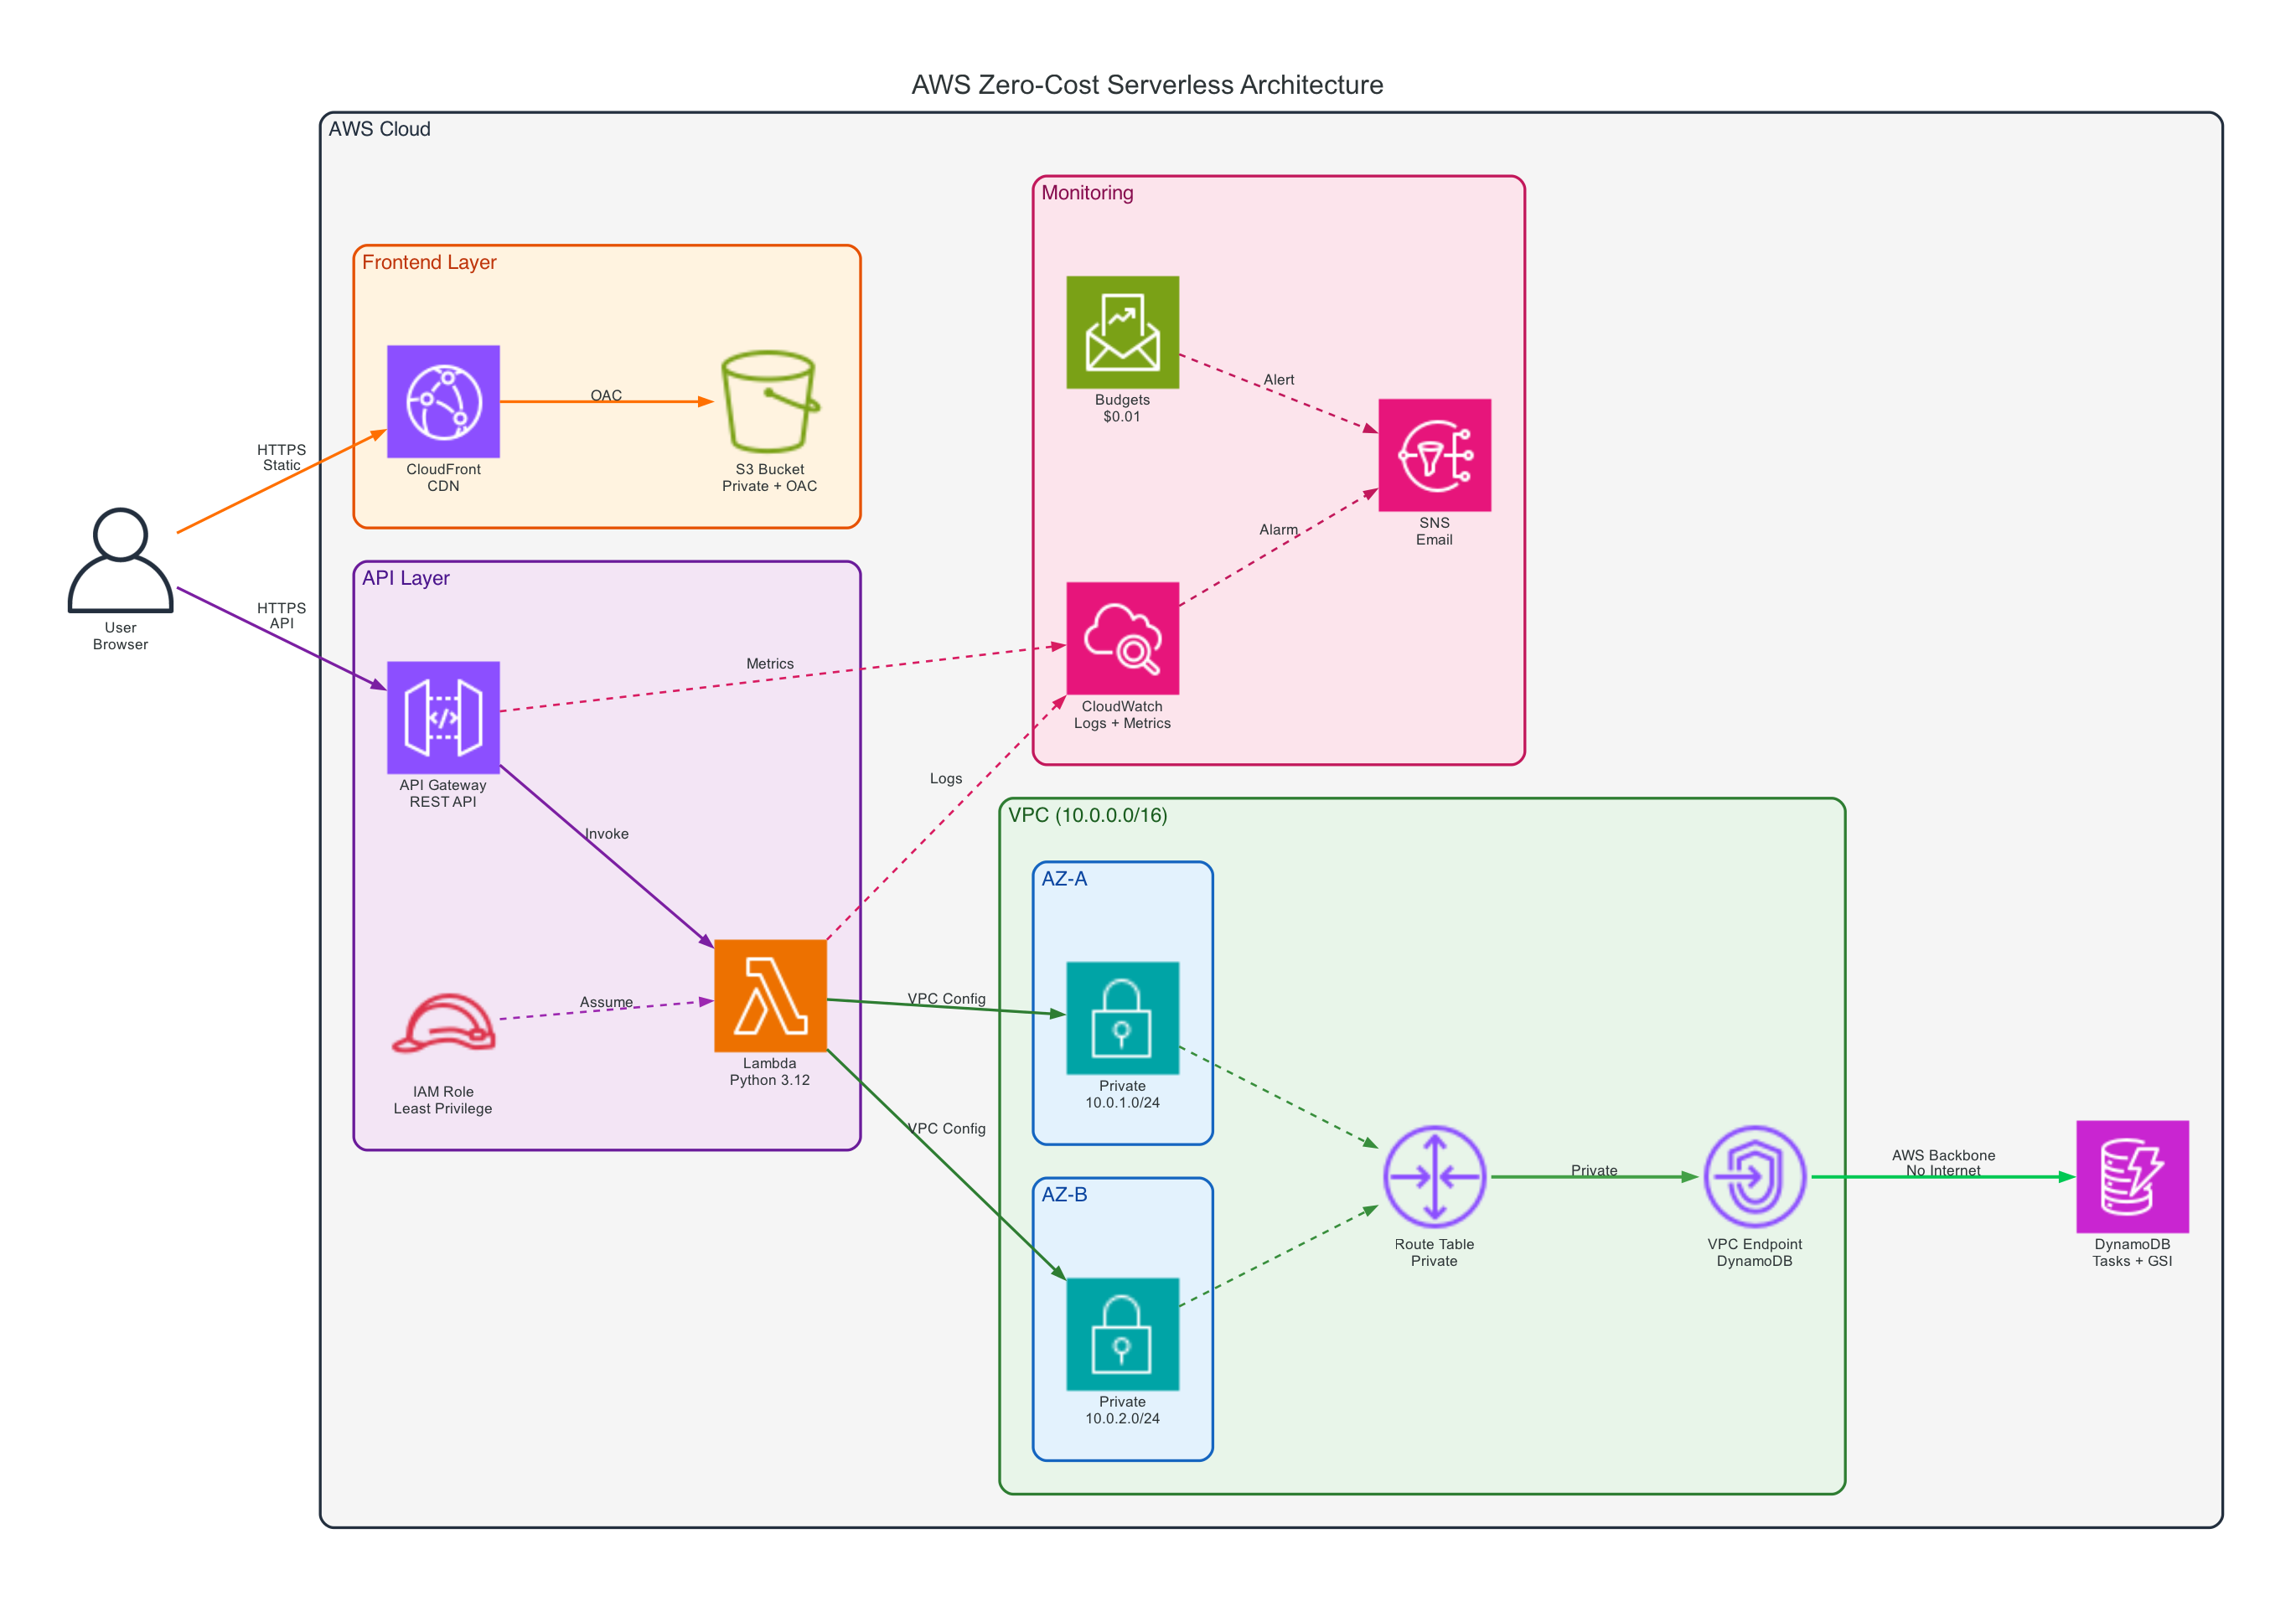
\includegraphics[width=\textwidth]{img/architecture_v3.png}
\caption{Sơ đồ kiến trúc tổng thể của hệ thống}
\label{fig:architecture_diagram}
\end{figure}

Kiến trúc được chia thành các layer chính:

\begin{itemize}
    \item \textbf{Frontend Layer:} CloudFront CDN phục vụ nội dung tĩnh từ S3 bucket private với Origin Access Control (OAC).
    
    \item \textbf{API Layer:} API Gateway nhận request từ client và kích hoạt Lambda function để xử lý logic nghiệp vụ.
    
    \item \textbf{Network Layer:} Custom VPC với 2 Private Subnets trải rộng trên 2 Availability Zones, VPC Gateway Endpoint cho DynamoDB.
    
    \item \textbf{Data Layer:} DynamoDB lưu trữ dữ liệu với Global Secondary Index để truy vấn hiệu quả.
    
    \item \textbf{Monitoring Layer:} CloudWatch, SNS và AWS Budgets để giám sát và kiểm soát chi phí.
\end{itemize}

\subsection{Luồng xử lý request}
\label{ssec:request_flow}

Khi người dùng tương tác với ứng dụng, có hai luồng xử lý chính:

\subsubsection{Luồng truy cập nội dung tĩnh (Static Assets)}

\begin{enumerate}
    \item Người dùng truy cập ứng dụng qua URL CloudFront (https://d1234567.cloudfront.net).
    \item CloudFront kiểm tra cache:
    \begin{itemize}
        \item \textbf{Cache HIT:} Nếu nội dung đã được cache, CloudFront trả về ngay lập tức từ edge location gần nhất, giảm độ trễ và không phát sinh request đến S3.
        \item \textbf{Cache MISS:} Nếu nội dung chưa có trong cache, CloudFront sử dụng Origin Access Control (OAC) để lấy file từ S3 bucket private.
    \end{itemize}
    \item S3 bucket policy chỉ cho phép CloudFront Service Principal đọc objects, từ chối mọi truy cập trực tiếp khác.
    \item CloudFront cache nội dung và trả về cho người dùng qua HTTPS.
\end{enumerate}

\subsubsection{Luồng xử lý API request}

\begin{enumerate}
    \item Người dùng thực hiện thao tác CRUD (ví dụ: tạo task mới) từ giao diện web.
    \item Browser gửi HTTPS request đến API Gateway endpoint (ví dụ: POST /tasks).
    \item API Gateway thực hiện:
    \begin{itemize}
        \item Kiểm tra CORS: Chỉ chấp nhận request từ CloudFront domain.
        \item Áp dụng throttling: Giới hạn 100 requests/second, burst 50 để bảo vệ backend.
        \item Kích hoạt Lambda function tương ứng.
    \end{itemize}
    \item Lambda function được khởi động (cold start nếu chưa có instance sẵn sàng, hoặc warm start nếu đã có):
    \begin{itemize}
        \item Lambda chạy trong VPC, được attach vào 2 Private Subnets (AZ-A và AZ-B) thông qua Elastic Network Interface (ENI).
        \item Lambda sử dụng IAM Role với quyền Least Privilege để truy cập DynamoDB.
    \end{itemize}
    \item Lambda gửi request đến DynamoDB:
    \begin{itemize}
        \item Traffic đi qua VPC Gateway Endpoint (vpce-xxxxx) thay vì Internet.
        \item Route Table của Private Subnets có entry: pl-xxxxx (DynamoDB Prefix List) → vpce-xxxxx.
        \item Security Group của Lambda chỉ cho phép outbound traffic đến port 443 của DynamoDB Prefix List.
        \item Traffic đi hoàn toàn trên AWS backbone network, không ra Internet công cộng.
    \end{itemize}
    \item DynamoDB xử lý request (GetItem, PutItem, UpdateItem, DeleteItem hoặc Query với GSI).
    \item Kết quả được trả về theo đường ngược lại: DynamoDB → VPC Endpoint → Lambda → API Gateway → Browser.
    \item CloudWatch tự động ghi log và metrics của Lambda và API Gateway.
\end{enumerate}

\subsection{Cơ chế Auto-scaling}
\label{ssec:autoscaling}

Một trong những ưu điểm lớn nhất của kiến trúc serverless là khả năng tự động mở rộng mà không cần cấu hình thủ công.

\subsubsection{Lambda Auto-scaling}

AWS Lambda tự động mở rộng theo số lượng request đồng thời:

\begin{itemize}
    \item \textbf{Cold Start:} Khi có request đầu tiên hoặc khi tất cả instances hiện tại đang bận, Lambda tạo một execution environment mới. Quá trình này mất khoảng 100-500ms cho Python runtime.
    
    \item \textbf{Warm Start:} Các request tiếp theo sử dụng lại execution environment đã có, thời gian phản hồi chỉ còn vài milliseconds.
    
    \item \textbf{Concurrent Execution:} Lambda tự động tạo thêm instances khi có nhiều request đồng thời. Mỗi instance xử lý một request tại một thời điểm.
    
    \item \textbf{Reserved Concurrency:} Để kiểm soát chi phí, nhóm đã cấu hình Reserved Concurrency = 50, giới hạn số lượng instances tối đa Lambda có thể tạo ra.
\end{itemize}

\subsubsection{API Gateway Load Balancing}

API Gateway hoạt động như một native load balancer:

\begin{itemize}
    \item Tự động phân phối request đến các Lambda instances khả dụng.
    \item Không cần Application Load Balancer (ALB) riêng biệt.
    \item Hỗ trợ throttling để bảo vệ backend khỏi traffic đột biến.
\end{itemize}

\subsubsection{DynamoDB Auto-scaling}

DynamoDB sử dụng chế độ On-Demand capacity:

\begin{itemize}
    \item Tự động điều chỉnh throughput dựa trên traffic thực tế.
    \item Không cần cấu hình provisioned capacity.
    \item Phù hợp với workload không dự đoán được.
    \item Nằm trong Free Tier: 25 GB storage, 25 RCU/WCU per month.
\end{itemize}

\subsection{High Availability Design}
\label{ssec:high_availability}

Hệ thống được thiết kế để đảm bảo tính sẵn sàng cao mà không cần cấu hình failover thủ công:

\begin{itemize}
    \item \textbf{Multi-AZ Deployment:} Lambda được deploy vào 2 Private Subnets nằm ở 2 Availability Zones khác nhau (ap-southeast-1a và ap-southeast-1b). Nếu một AZ gặp sự cố, Lambda vẫn có thể chạy ở AZ còn lại.
    
    \item \textbf{DynamoDB Multi-AZ Replication:} DynamoDB tự động replicate dữ liệu across multiple AZs trong cùng region, đảm bảo durability 99.999999999\% (11 nines).
    
    \item \textbf{CloudFront Global Edge Network:} CloudFront có hơn 400 edge locations trên toàn cầu, tự động route traffic đến edge location gần nhất và khỏe mạnh nhất.
    
    \item \textbf{API Gateway Regional Endpoint:} API Gateway tự động replicate across AZs trong region.
\end{itemize}

\subsection{Bảo mật theo nguyên tắc Defense-in-Depth}
\label{ssec:security_layers}

Hệ thống áp dụng nhiều lớp bảo mật:

\begin{enumerate}
    \item \textbf{Network Layer:}
    \begin{itemize}
        \item Lambda chạy trong Private Subnets, không có Internet Gateway.
        \item Security Group chỉ cho phép outbound đến DynamoDB Prefix List port 443.
        \item VPC Gateway Endpoint đảm bảo traffic không ra Internet.
        \item Không có NAT Gateway (tránh chi phí \$32/month và giảm attack surface).
    \end{itemize}
    
    \item \textbf{Application Layer:}
    \begin{itemize}
        \item S3 bucket ở chế độ private, tất cả 4 Block Public Access options được bật.
        \item CloudFront OAC đảm bảo chỉ CloudFront mới có thể đọc từ S3.
        \item API Gateway CORS chỉ chấp nhận request từ CloudFront domain cụ thể.
        \item API Gateway throttling bảo vệ khỏi DDoS.
    \end{itemize}
    
    \item \textbf{Identity Layer:}
    \begin{itemize}
        \item Mỗi Lambda function có IAM Role riêng biệt.
        \item IAM Policy áp dụng Least Privilege: chỉ cấp quyền tối thiểu cần thiết.
        \item Resource-based policy: chỉ định chính xác DynamoDB table ARN, không dùng wildcard (*).
    \end{itemize}
    
    \item \textbf{Data Layer:}
    \begin{itemize}
        \item DynamoDB encryption at rest được bật mặc định.
        \item Tất cả traffic đều qua HTTPS/TLS.
    \end{itemize}
\end{enumerate}

\subsection{Chiến lược Zero-Cost}
\label{ssec:zero_cost}

Để đảm bảo chi phí bằng 0, nhóm đã áp dụng các biện pháp sau:

\begin{itemize}
    \item \textbf{Không sử dụng NAT Gateway:} Thay vào đó sử dụng VPC Gateway Endpoint (miễn phí) để Lambda kết nối DynamoDB.
    
    \item \textbf{Lambda Reserved Concurrency = 50:} Giới hạn số lượng instances đồng thời để tránh vượt Free Tier (1 triệu requests/month, 400,000 GB-seconds compute).
    
    \item \textbf{API Gateway Throttling:} Giới hạn 100 req/s, burst 50 để kiểm soát traffic.
    
    \item \textbf{DynamoDB On-Demand:} Nằm trong Free Tier: 25 GB storage, 25 RCU/WCU.
    
    \item \textbf{CloudFront Free Tier:} 1 TB data transfer out, 10 triệu HTTP/HTTPS requests.
    
    \item \textbf{S3 Free Tier:} 5 GB storage, 20,000 GET requests, 2,000 PUT requests.
    
    \item \textbf{AWS Budgets:} Cấu hình budget \$0.01 với alerts ở 80\% và 100\% để phát hiện sớm nếu có chi phí phát sinh.
\end{itemize}

\section{Triển khai hệ thống}
\label{sec:implementation}

\subsection{Frontend Layer}
\label{ssec:frontend_impl}

\subsubsection{Phát triển giao diện người dùng}

Frontend được xây dựng bằng HTML, CSS và JavaScript thuần, không sử dụng framework phức tạp để đảm bảo đơn giản và dễ triển khai. Giao diện cung cấp đầy đủ các chức năng CRUD cho quản lý công việc:

\begin{itemize}
    \item \textbf{Tạo task mới:} Form nhập liệu với các trường: title, description, priority (low/medium/high), dueDate, status (pending/done).
    \item \textbf{Hiển thị danh sách tasks:} Table responsive hiển thị tất cả tasks với khả năng sắp xếp.
    \item \textbf{Cập nhật task:} Click vào task để chỉnh sửa thông tin.
    \item \textbf{Xóa task:} Nút delete với confirmation dialog.
    \item \textbf{Lọc tasks:} Filter theo priority và dueDate.
\end{itemize}

Frontend gọi API thông qua JavaScript Fetch API, gửi request đến API Gateway endpoint.

\subsubsection{Triển khai S3 và CloudFront}

\textbf{Bước 1: Tạo S3 Bucket}

\begin{itemize}
    \item Tạo S3 bucket với tên unique (ví dụ: task-manager-frontend-2024).
    \item \textbf{QUAN TRỌNG:} Bật tất cả 4 Block Public Access options:
    \begin{itemize}
        \item Block all public access
        \item Block public access to buckets and objects granted through new access control lists (ACLs)
        \item Block public access to buckets and objects granted through any access control lists (ACLs)
        \item Block public access to buckets and objects granted through new public bucket or access point policies
    \end{itemize}
    \item \textbf{KHÔNG} bật Static Website Hosting.
    \item Upload các file HTML, CSS, JS vào bucket.
\end{itemize}

\textbf{Bước 2: Tạo CloudFront Distribution}

\begin{itemize}
    \item Origin domain: Chọn S3 bucket vừa tạo.
    \item \textbf{Origin Access:} Chọn "Origin access control settings (recommended)".
    \item Tạo OAC mới với tên mô tả rõ ràng (ví dụ: task-manager-oac).
    \item Default root object: index.html
    \item Viewer protocol policy: Redirect HTTP to HTTPS.
    \item Allowed HTTP methods: GET, HEAD, OPTIONS.
    \item Cache policy: CachingOptimized.
\end{itemize}

\textbf{Bước 3: Cập nhật S3 Bucket Policy}

Sau khi tạo CloudFront distribution, AWS sẽ đề xuất bucket policy. Copy và apply policy này vào S3 bucket:

\begin{verbatim}
{
  "Version": "2012-10-17",
  "Statement": [
    {
      "Sid": "AllowCloudFrontServicePrincipal",
      "Effect": "Allow",
      "Principal": {
        "Service": "cloudfront.amazonaws.com"
      },
      "Action": "s3:GetObject",
      "Resource": "arn:aws:s3:::bucket-name/*",
      "Condition": {
        "StringEquals": {
          "AWS:SourceArn": "arn:aws:cloudfront::account-id:distribution/distribution-id"
        }
      }
    }
  ]
}
\end{verbatim}

Policy này đảm bảo chỉ CloudFront distribution cụ thể mới có thể đọc objects từ S3.

\subsection{Backend API Layer}
\label{ssec:backend_impl}

\subsubsection{Lambda Function Implementation}

Lambda function được viết bằng Python 3.12, xử lý tất cả 4 operations CRUD:

\begin{itemize}
    \item \textbf{GET /tasks:} Query tất cả tasks của user từ DynamoDB sử dụng GSI userId-index.
    \item \textbf{POST /tasks:} Tạo task mới với taskId = UUID, lưu vào DynamoDB.
    \item \textbf{PUT /tasks/\{id\}:} Update task theo taskId.
    \item \textbf{DELETE /tasks/\{id\}:} Xóa task theo taskId.
\end{itemize}

Code structure:

\begin{verbatim}
def lambda_handler(event, context):
    http_method = event['httpMethod']
    path = event['path']
    
    if http_method == 'GET' and path == '/tasks':
        return get_tasks(event)
    elif http_method == 'POST' and path == '/tasks':
        return create_task(event)
    elif http_method == 'PUT':
        return update_task(event)
    elif http_method == 'DELETE':
        return delete_task(event)
\end{verbatim}

\subsubsection{API Gateway Configuration}

\begin{itemize}
    \item \textbf{API Type:} REST API (không dùng HTTP API).
    \item \textbf{Resources:} Tạo resource /tasks và /tasks/\{id\}.
    \item \textbf{Methods:} GET, POST, PUT, DELETE với Lambda integration.
    \item \textbf{CORS Configuration:}
    \begin{itemize}
        \item Access-Control-Allow-Origin: https://d1234567.cloudfront.net (CloudFront domain cụ thể)
        \item Access-Control-Allow-Methods: GET, POST, PUT, DELETE, OPTIONS
        \item Access-Control-Allow-Headers: Content-Type
    \end{itemize}
    \item \textbf{Throttling Settings:}
    \begin{itemize}
        \item Rate limit: 100 requests/second
        \item Burst limit: 50 requests
    \end{itemize}
    \item \textbf{Deployment Stage:} prod
\end{itemize}

\subsection{Network Layer}
\label{ssec:network_impl}

\subsubsection{VPC Configuration}

\textbf{Bước 1: Tạo Custom VPC}

\begin{itemize}
    \item VPC CIDR: 10.0.0.0/16
    \item Enable DNS hostnames: Yes
    \item Enable DNS resolution: Yes
\end{itemize}

\textbf{Bước 2: Tạo Private Subnets}

\begin{itemize}
    \item \textbf{Private Subnet A:}
    \begin{itemize}
        \item CIDR: 10.0.1.0/24
        \item Availability Zone: ap-southeast-1a
        \item Auto-assign public IPv4: No
    \end{itemize}
    \item \textbf{Private Subnet B:}
    \begin{itemize}
        \item CIDR: 10.0.2.0/24
        \item Availability Zone: ap-southeast-1b
        \item Auto-assign public IPv4: No
    \end{itemize}
\end{itemize}

\textbf{Bước 3: Tạo Route Table}

\begin{itemize}
    \item Tạo Private Route Table.
    \item Associate với cả 2 Private Subnets.
    \item \textbf{KHÔNG} tạo Internet Gateway.
    \item \textbf{KHÔNG} tạo NAT Gateway.
\end{itemize}

\subsubsection{VPC Gateway Endpoint for DynamoDB}

\textbf{Bước 1: Tạo VPC Endpoint}

\begin{itemize}
    \item Service category: AWS services
    \item Service name: com.amazonaws.ap-southeast-1.dynamodb
    \item VPC: Chọn Custom VPC vừa tạo
    \item Route tables: Chọn Private Route Table
    \item Policy: Full access (hoặc custom policy nếu cần)
\end{itemize}

Sau khi tạo, VPC Endpoint sẽ tự động thêm route vào Route Table:
\begin{itemize}
    \item Destination: pl-xxxxx (DynamoDB Prefix List)
    \item Target: vpce-xxxxx (VPC Endpoint ID)
\end{itemize}

\textbf{Bước 2: Tạo Security Group cho Lambda}

\begin{itemize}
    \item Name: lambda-sg
    \item VPC: Custom VPC
    \item \textbf{Inbound rules:} Không cần (Lambda không nhận inbound traffic)
    \item \textbf{Outbound rules:}
    \begin{itemize}
        \item Type: HTTPS
        \item Protocol: TCP
        \item Port: 443
        \item Destination: pl-xxxxx (DynamoDB Prefix List)
    \end{itemize}
\end{itemize}

\textbf{Bước 3: Attach Lambda to VPC}

Trong Lambda configuration:
\begin{itemize}
    \item VPC: Chọn Custom VPC
    \item Subnets: Chọn cả Private Subnet A và Private Subnet B
    \item Security groups: Chọn lambda-sg
\end{itemize}

Khi Lambda được attach vào VPC, AWS sẽ tạo Elastic Network Interface (ENI) trong các subnets. Quá trình này mất khoảng 1-2 phút.

\subsection{Database Layer}
\label{ssec:database_impl}

\subsubsection{DynamoDB Table Creation}

\begin{itemize}
    \item \textbf{Table name:} Tasks
    \item \textbf{Partition key:} taskId (String)
    \item \textbf{Table settings:} On-demand capacity mode
    \item \textbf{Encryption:} AWS owned key (default, miễn phí)
\end{itemize}

\subsubsection{Global Secondary Index (GSI)}

Để query tasks theo userId hiệu quả, tạo GSI:

\begin{itemize}
    \item \textbf{Index name:} userId-index
    \item \textbf{Partition key:} userId (String)
    \item \textbf{Sort key:} createdAt (String) - optional, để sắp xếp theo thời gian
    \item \textbf{Projection type:} ALL (project tất cả attributes)
\end{itemize}

Với GSI này, Lambda có thể query nhanh chóng:
\begin{verbatim}
response = dynamodb.query(
    TableName='Tasks',
    IndexName='userId-index',
    KeyConditionExpression='userId = :uid',
    ExpressionAttributeValues={':uid': user_id}
)
\end{verbatim}

\subsection{IAM Security Layer}
\label{ssec:iam_impl}

\subsubsection{Lambda Task Role}

Tạo IAM Role cho Lambda function xử lý tasks:

\textbf{Trust Policy:}
\begin{verbatim}
{
  "Version": "2012-10-17",
  "Statement": [
    {
      "Effect": "Allow",
      "Principal": {"Service": "lambda.amazonaws.com"},
      "Action": "sts:AssumeRole"
    }
  ]
}
\end{verbatim}

\textbf{Permissions Policy (Inline):}
\begin{verbatim}
{
  "Version": "2012-10-17",
  "Statement": [
    {
      "Effect": "Allow",
      "Action": [
        "dynamodb:GetItem",
        "dynamodb:PutItem",
        "dynamodb:UpdateItem",
        "dynamodb:DeleteItem",
        "dynamodb:Query",
        "dynamodb:Scan"
      ],
      "Resource": [
        "arn:aws:dynamodb:ap-southeast-1:123456789012:table/Tasks",
        "arn:aws:dynamodb:ap-southeast-1:123456789012:table/Tasks/index/*"
      ]
    },
    {
      "Effect": "Allow",
      "Action": [
        "logs:CreateLogGroup",
        "logs:CreateLogStream",
        "logs:PutLogEvents"
      ],
      "Resource": "arn:aws:logs:ap-southeast-1:123456789012:log-group:/aws/lambda/*"
    },
    {
      "Effect": "Allow",
      "Action": [
        "ec2:CreateNetworkInterface",
        "ec2:DescribeNetworkInterfaces",
        "ec2:DeleteNetworkInterface"
      ],
      "Resource": "*"
    }
  ]
}
\end{verbatim}

\textbf{Giải thích các permissions:}
\begin{itemize}
    \item \textbf{DynamoDB actions:} Chỉ cấp quyền trên table Tasks cụ thể, không dùng wildcard.
    \item \textbf{CloudWatch Logs:} Để Lambda ghi logs.
    \item \textbf{EC2 Network Interface:} Bắt buộc khi Lambda chạy trong VPC để tạo ENI.
\end{itemize}

\subsubsection{Lambda Base Role}

Nếu có Lambda functions khác không cần truy cập DynamoDB, tạo role riêng chỉ với CloudWatch Logs và EC2 ENI permissions.

\section{Bằng chứng bảo mật}
\label{sec:security}

Phần này cung cấp bằng chứng chi tiết về các biện pháp bảo mật đã được triển khai trong hệ thống, bao gồm screenshots và giải thích cho từng yêu cầu bảo mật.

\subsection{Frontend Security Evidence}
\label{ssec:frontend_security}

\subsubsection{SE-1: S3 Block Public Access Enabled}

Hình \ref{fig:se1} cho thấy S3 bucket đã được cấu hình với tất cả 4 Block Public Access options được bật. Điều này đảm bảo bucket hoàn toàn private và không thể truy cập trực tiếp từ Internet.

\begin{figure}[H]
\centering
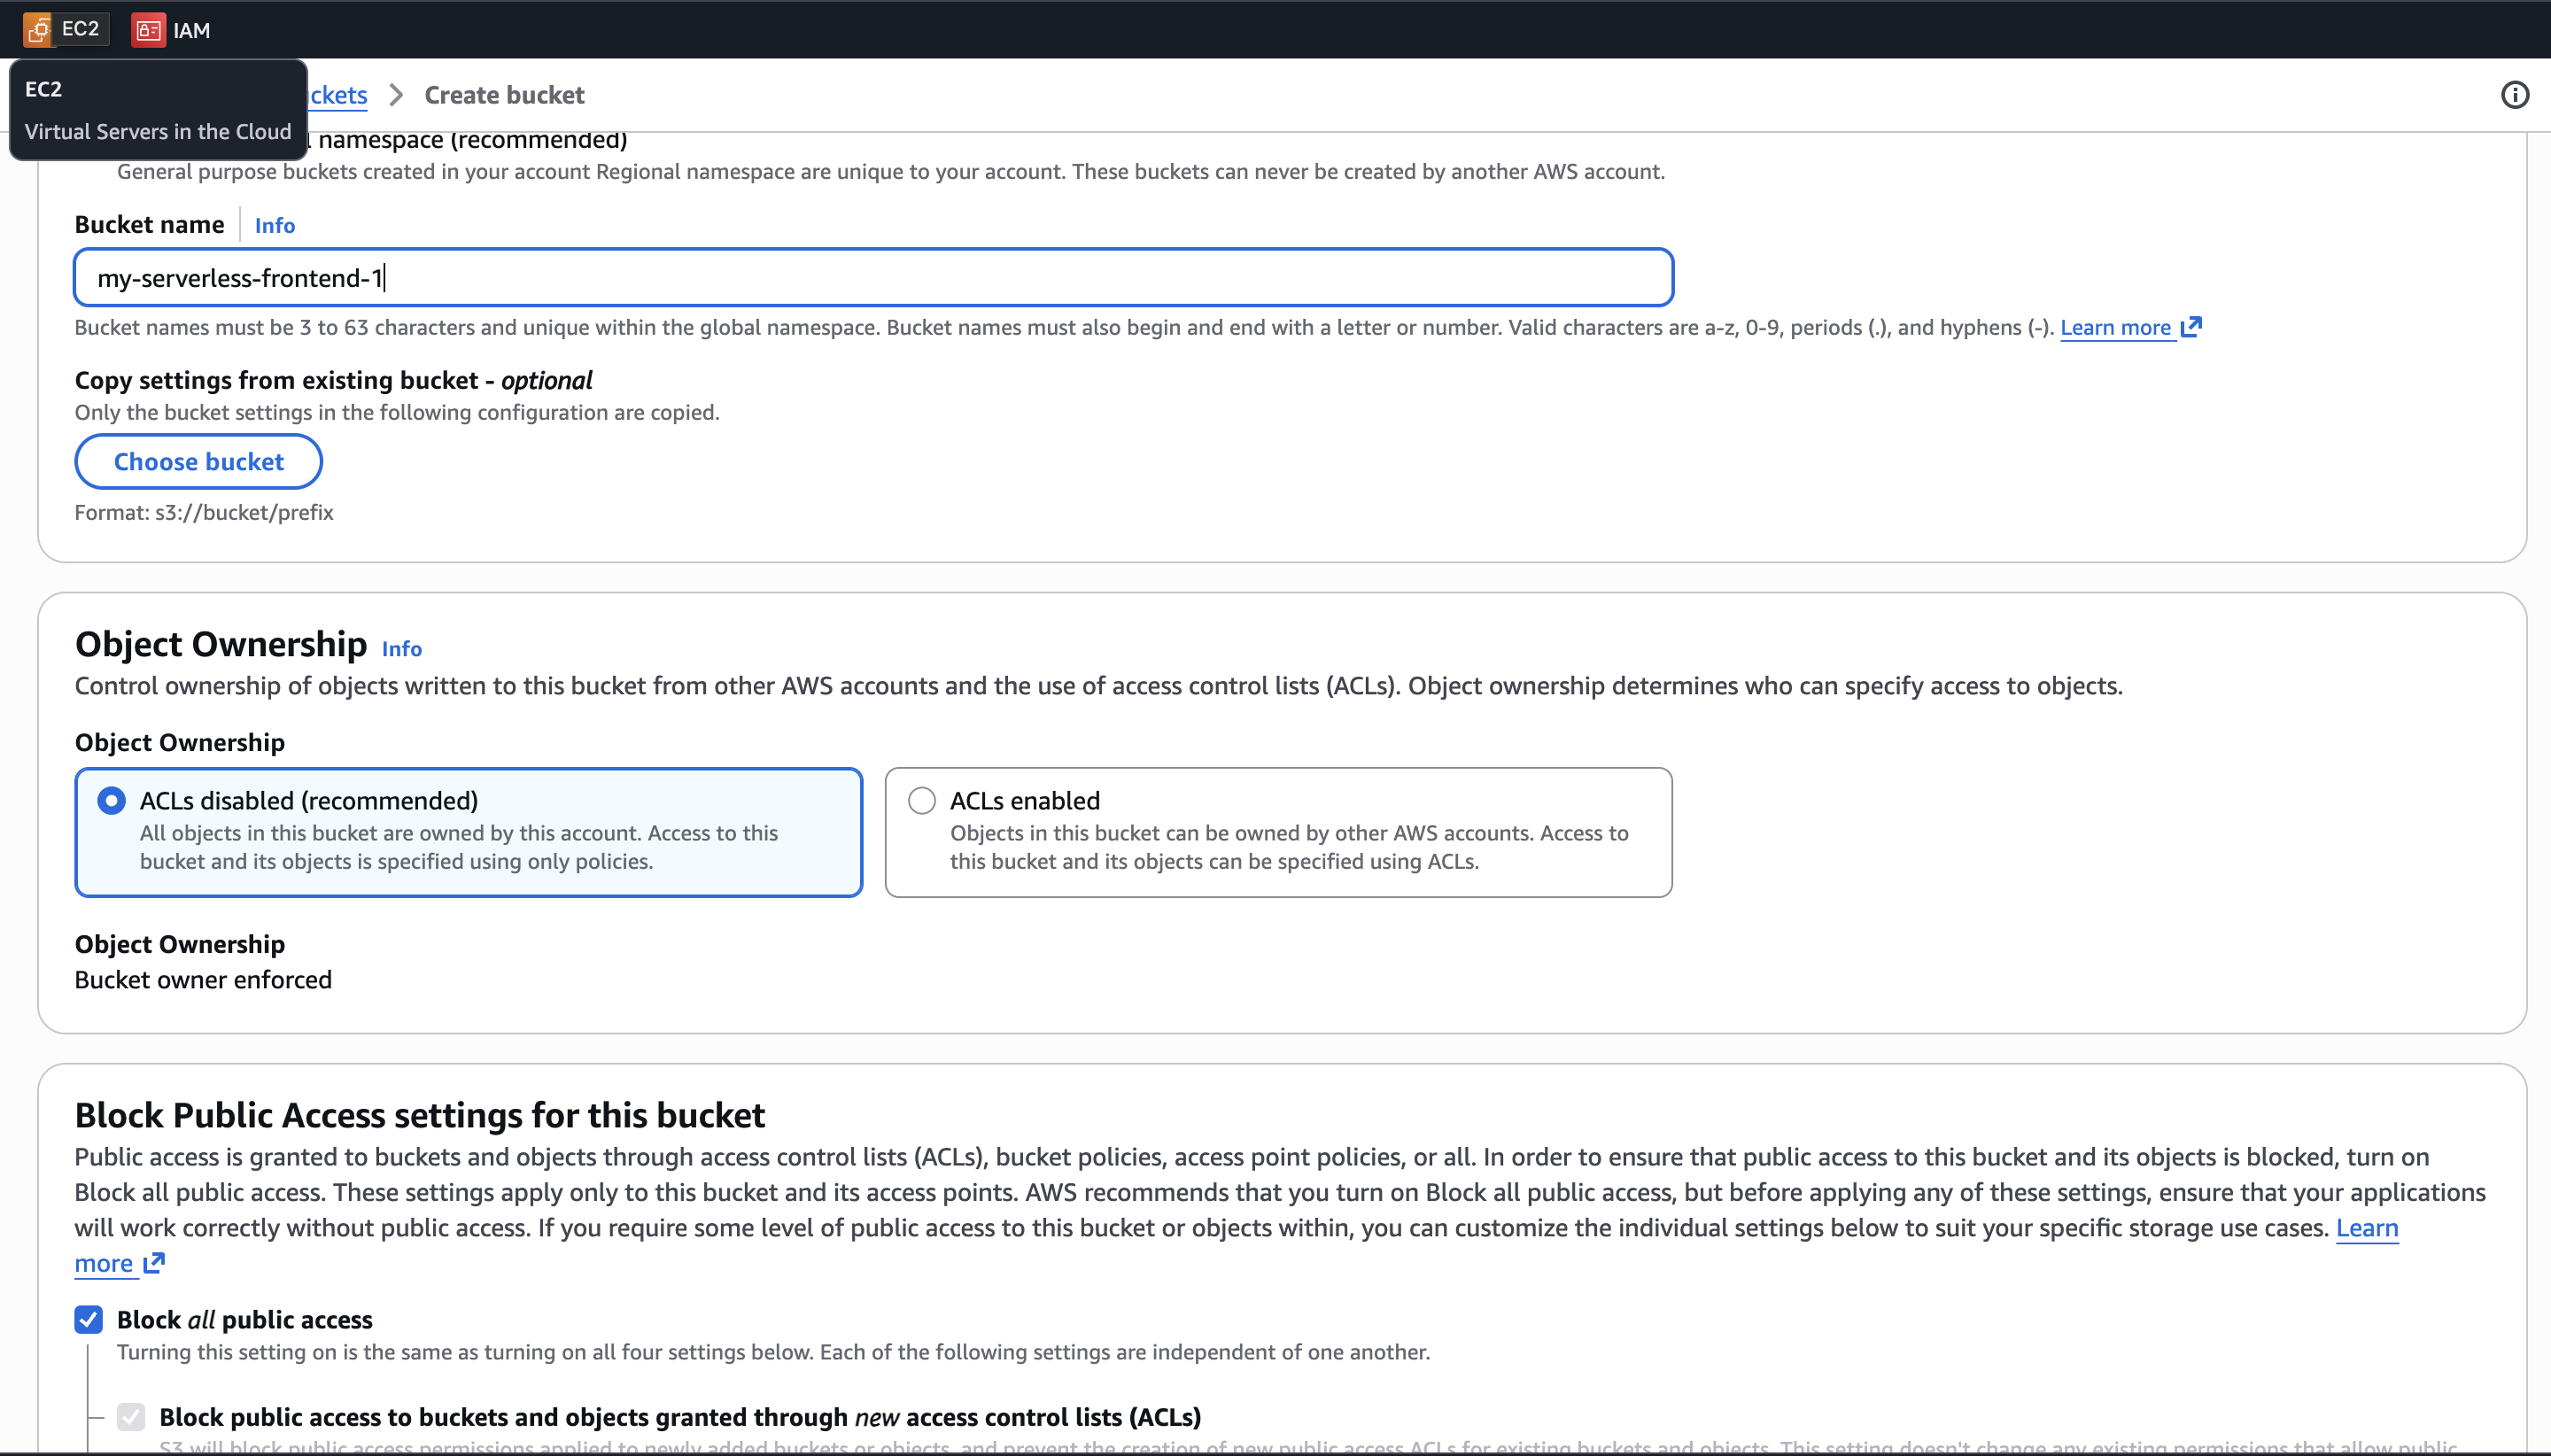
\includegraphics[width=0.9\textwidth]{img/SE-1_s3_block_public_access.png}
\caption{S3 Block Public Access - Tất cả 4 options được bật}
\label{fig:se1}
\end{figure}

Các options được bật:
\begin{itemize}
    \item Block all public access
    \item Block public access to buckets and objects granted through new ACLs
    \item Block public access to buckets and objects granted through any ACLs
    \item Block public access to buckets and objects granted through new public bucket or access point policies
\end{itemize}

\subsubsection{SE-2: Direct S3 Access Rejected}

Hình \ref{fig:se2} minh chứng rằng khi truy cập trực tiếp vào S3 URL, request bị từ chối với mã lỗi 403 Forbidden. Điều này xác nhận bucket không thể truy cập công khai.

\begin{figure}[H]
\centering
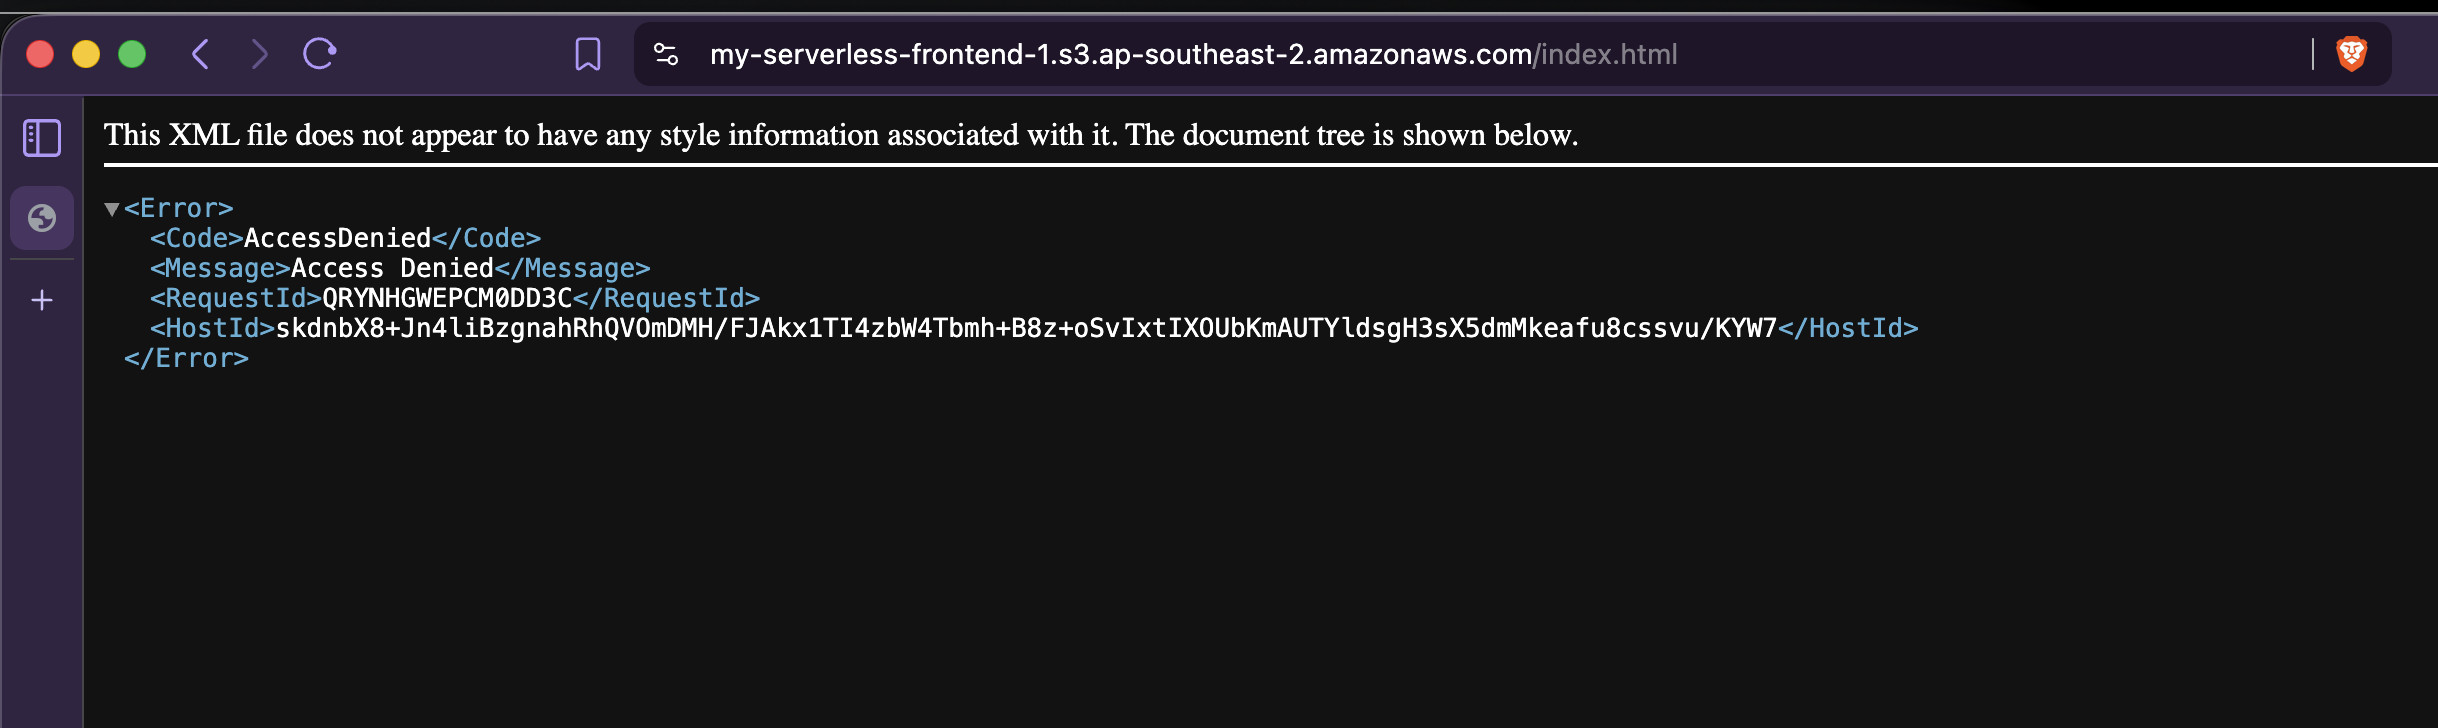
\includegraphics[width=0.9\textwidth]{img/SE-2_s3_403_forbidden.png}
\caption{Truy cập trực tiếp S3 URL bị từ chối với 403 Forbidden}
\label{fig:se2}
\end{figure}

Test command đã thực hiện:
\begin{verbatim}
curl https://bucket-name.s3.ap-southeast-1.amazonaws.com/index.html
\end{verbatim}

Kết quả: Access Denied - xác nhận S3 bucket đã được bảo vệ đúng cách.

\subsubsection{SE-3: CloudFront Access Succeeds}

Hình \ref{fig:se3} cho thấy khi truy cập qua CloudFront URL, ứng dụng hoạt động bình thường với status code 200 OK. Điều này chứng minh CloudFront có thể đọc từ S3 thông qua OAC.

\begin{figure}[H]
\centering
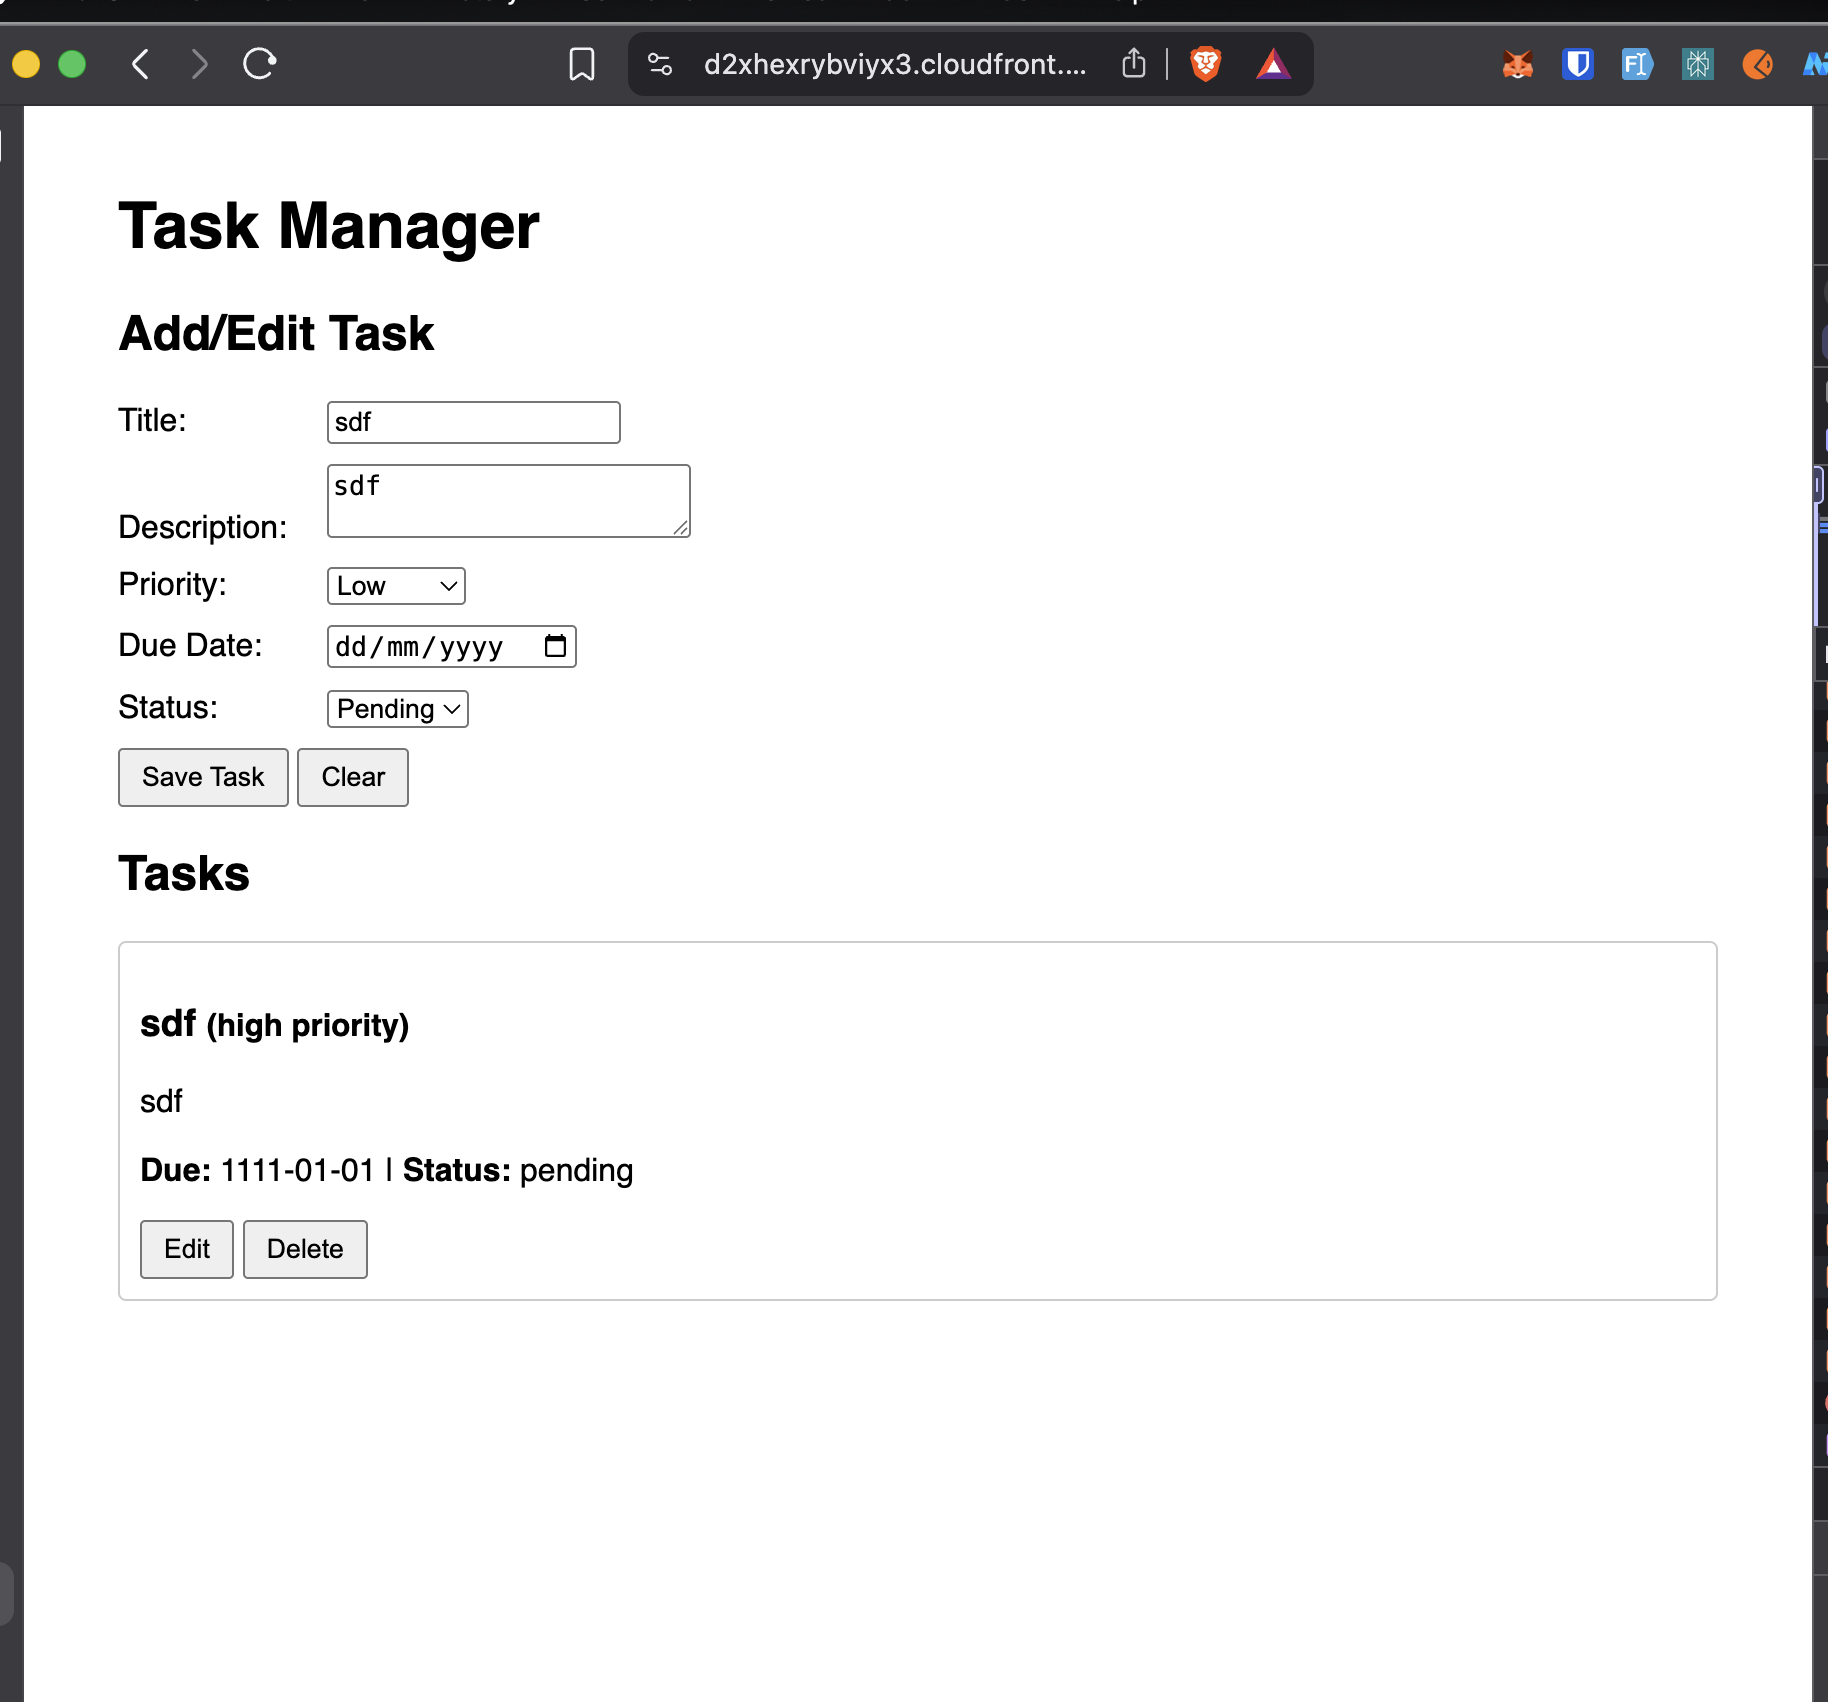
\includegraphics[width=0.9\textwidth]{img/SE-3_cloudfront_200.png}
\caption{Truy cập qua CloudFront URL thành công với 200 OK}
\label{fig:se3}
\end{figure}

CloudFront URL: https://d1234567.cloudfront.net

\subsubsection{SE-4: OAC Attached to CloudFront}

Hình \ref{fig:se4a} và \ref{fig:se4b} hiển thị cấu hình CloudFront distribution với Origin Access Control (OAC) được attach. OAC cho phép CloudFront đọc từ S3 private bucket một cách an toàn.

\begin{figure}[H]
\centering
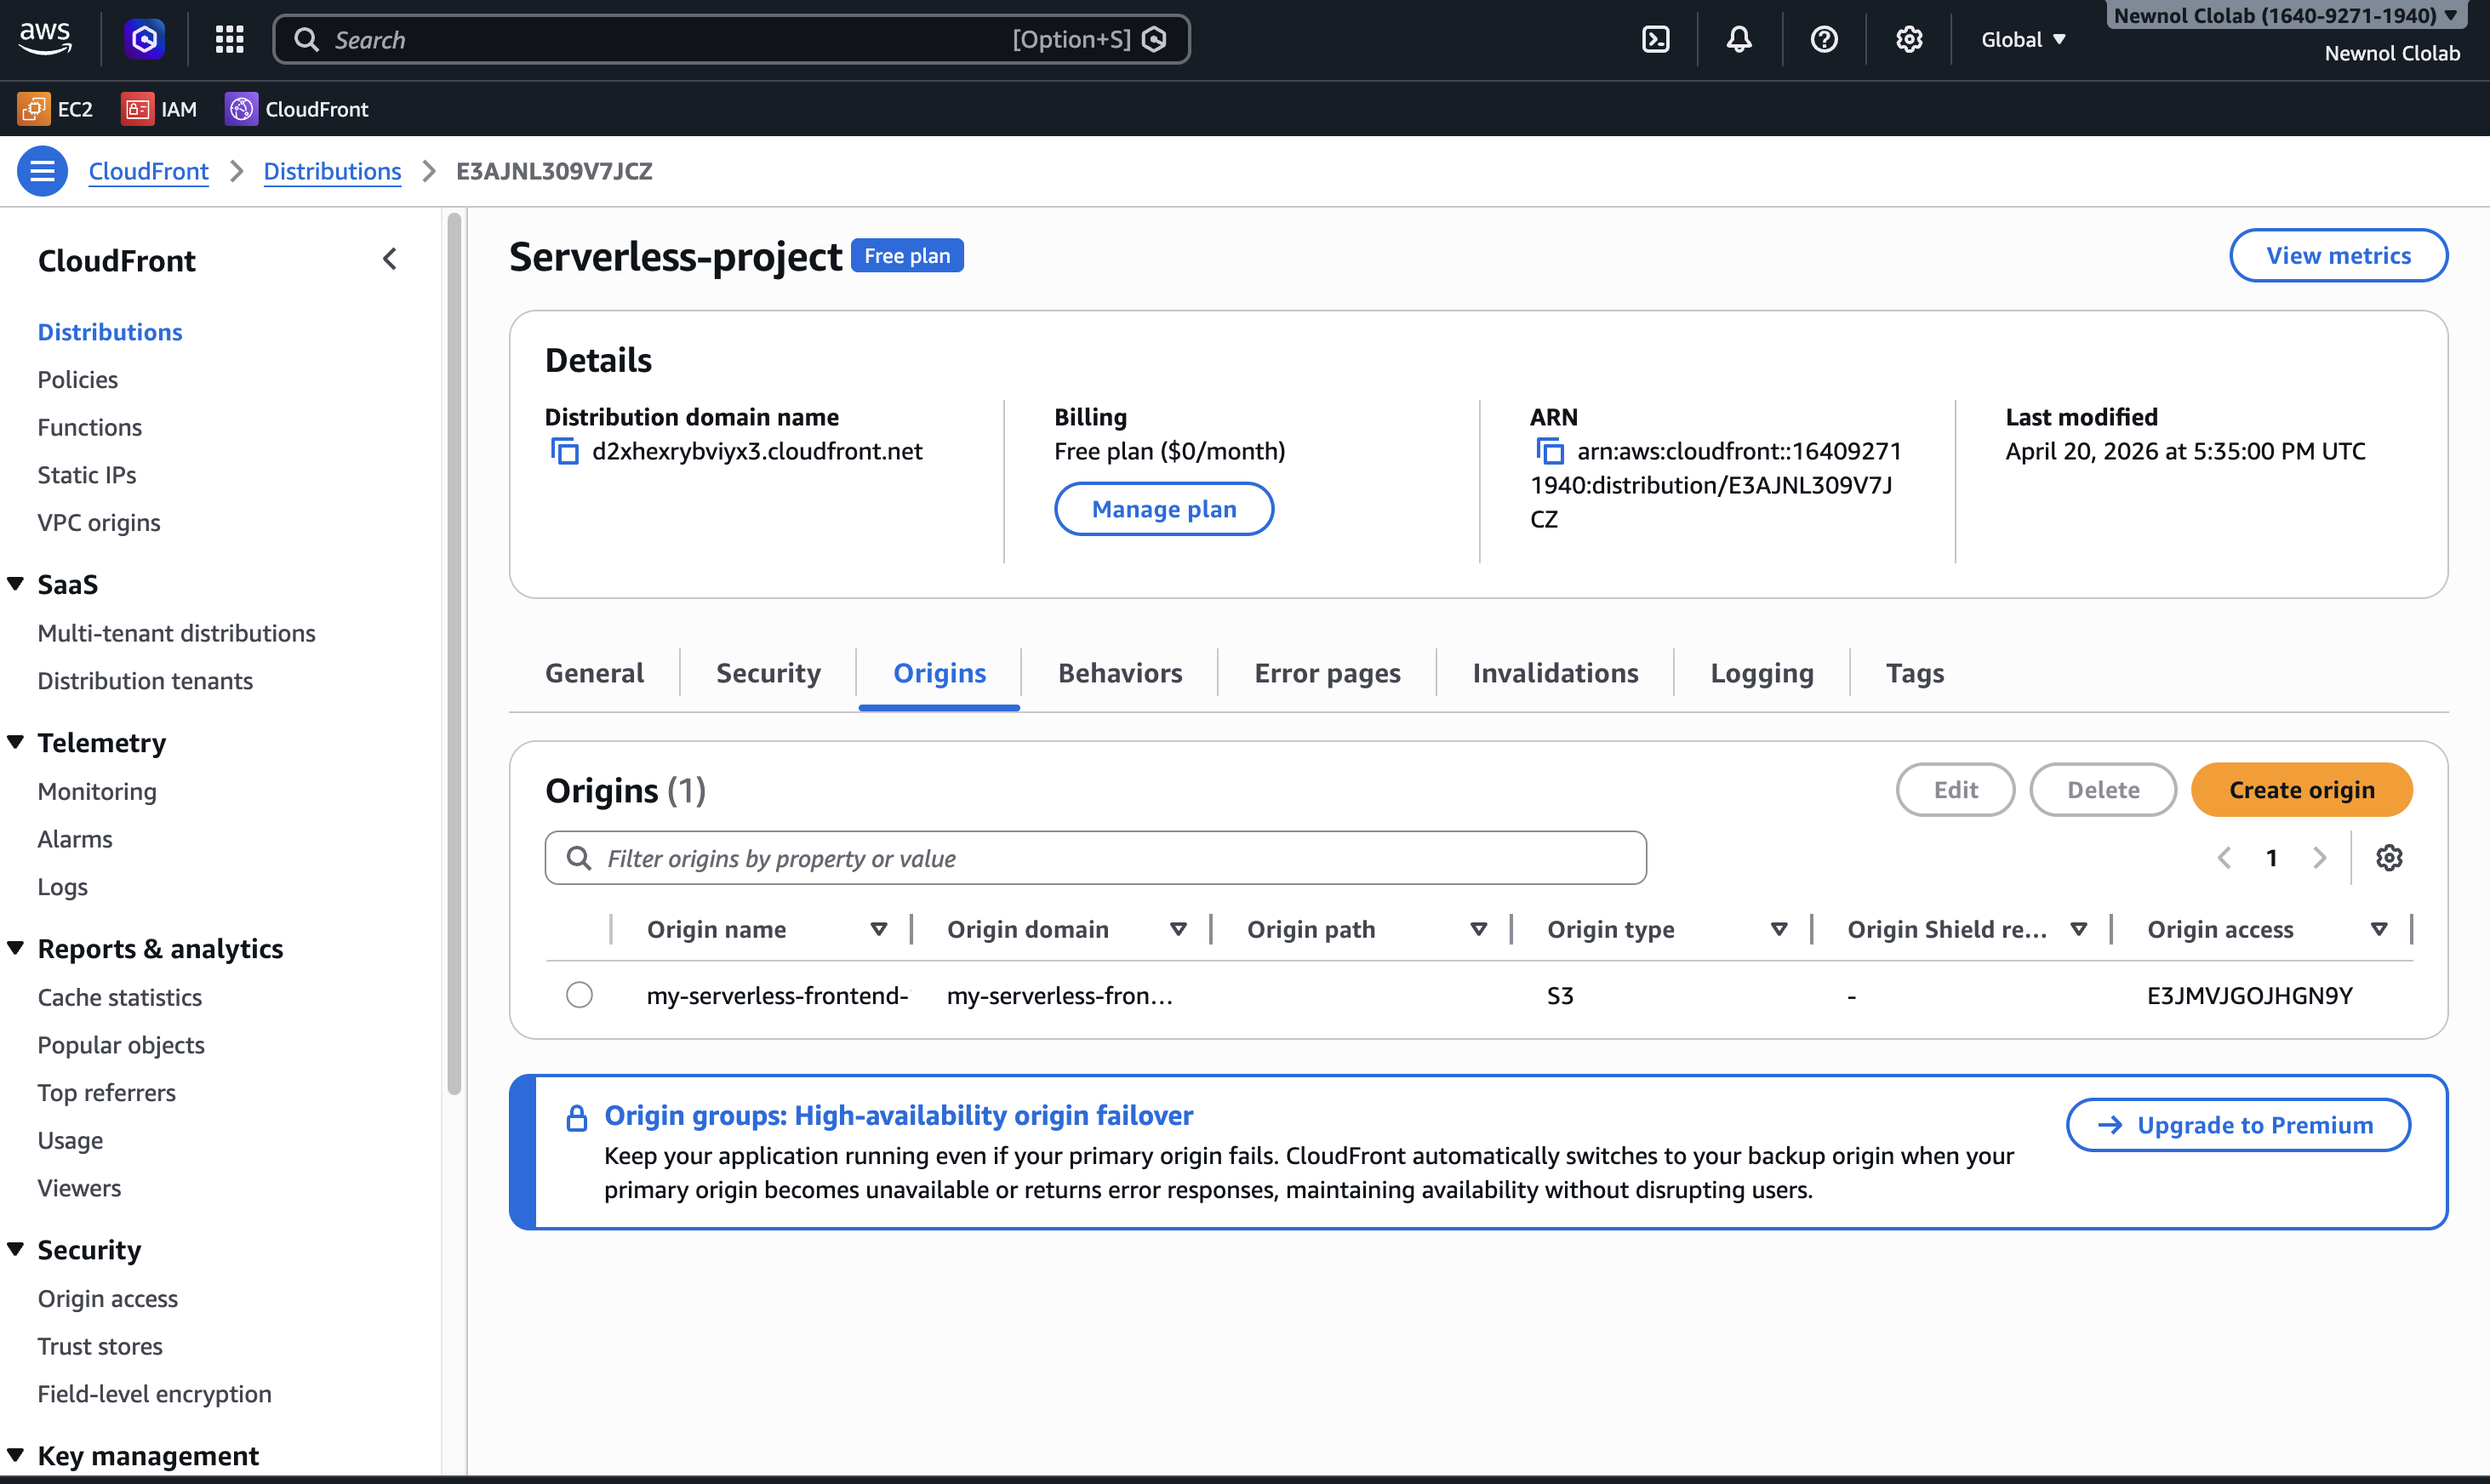
\includegraphics[width=0.9\textwidth]{img/SE-4_cloudfront_oac_1.png}
\caption{CloudFront Origin settings với OAC}
\label{fig:se4a}
\end{figure}

\begin{figure}[H]
\centering
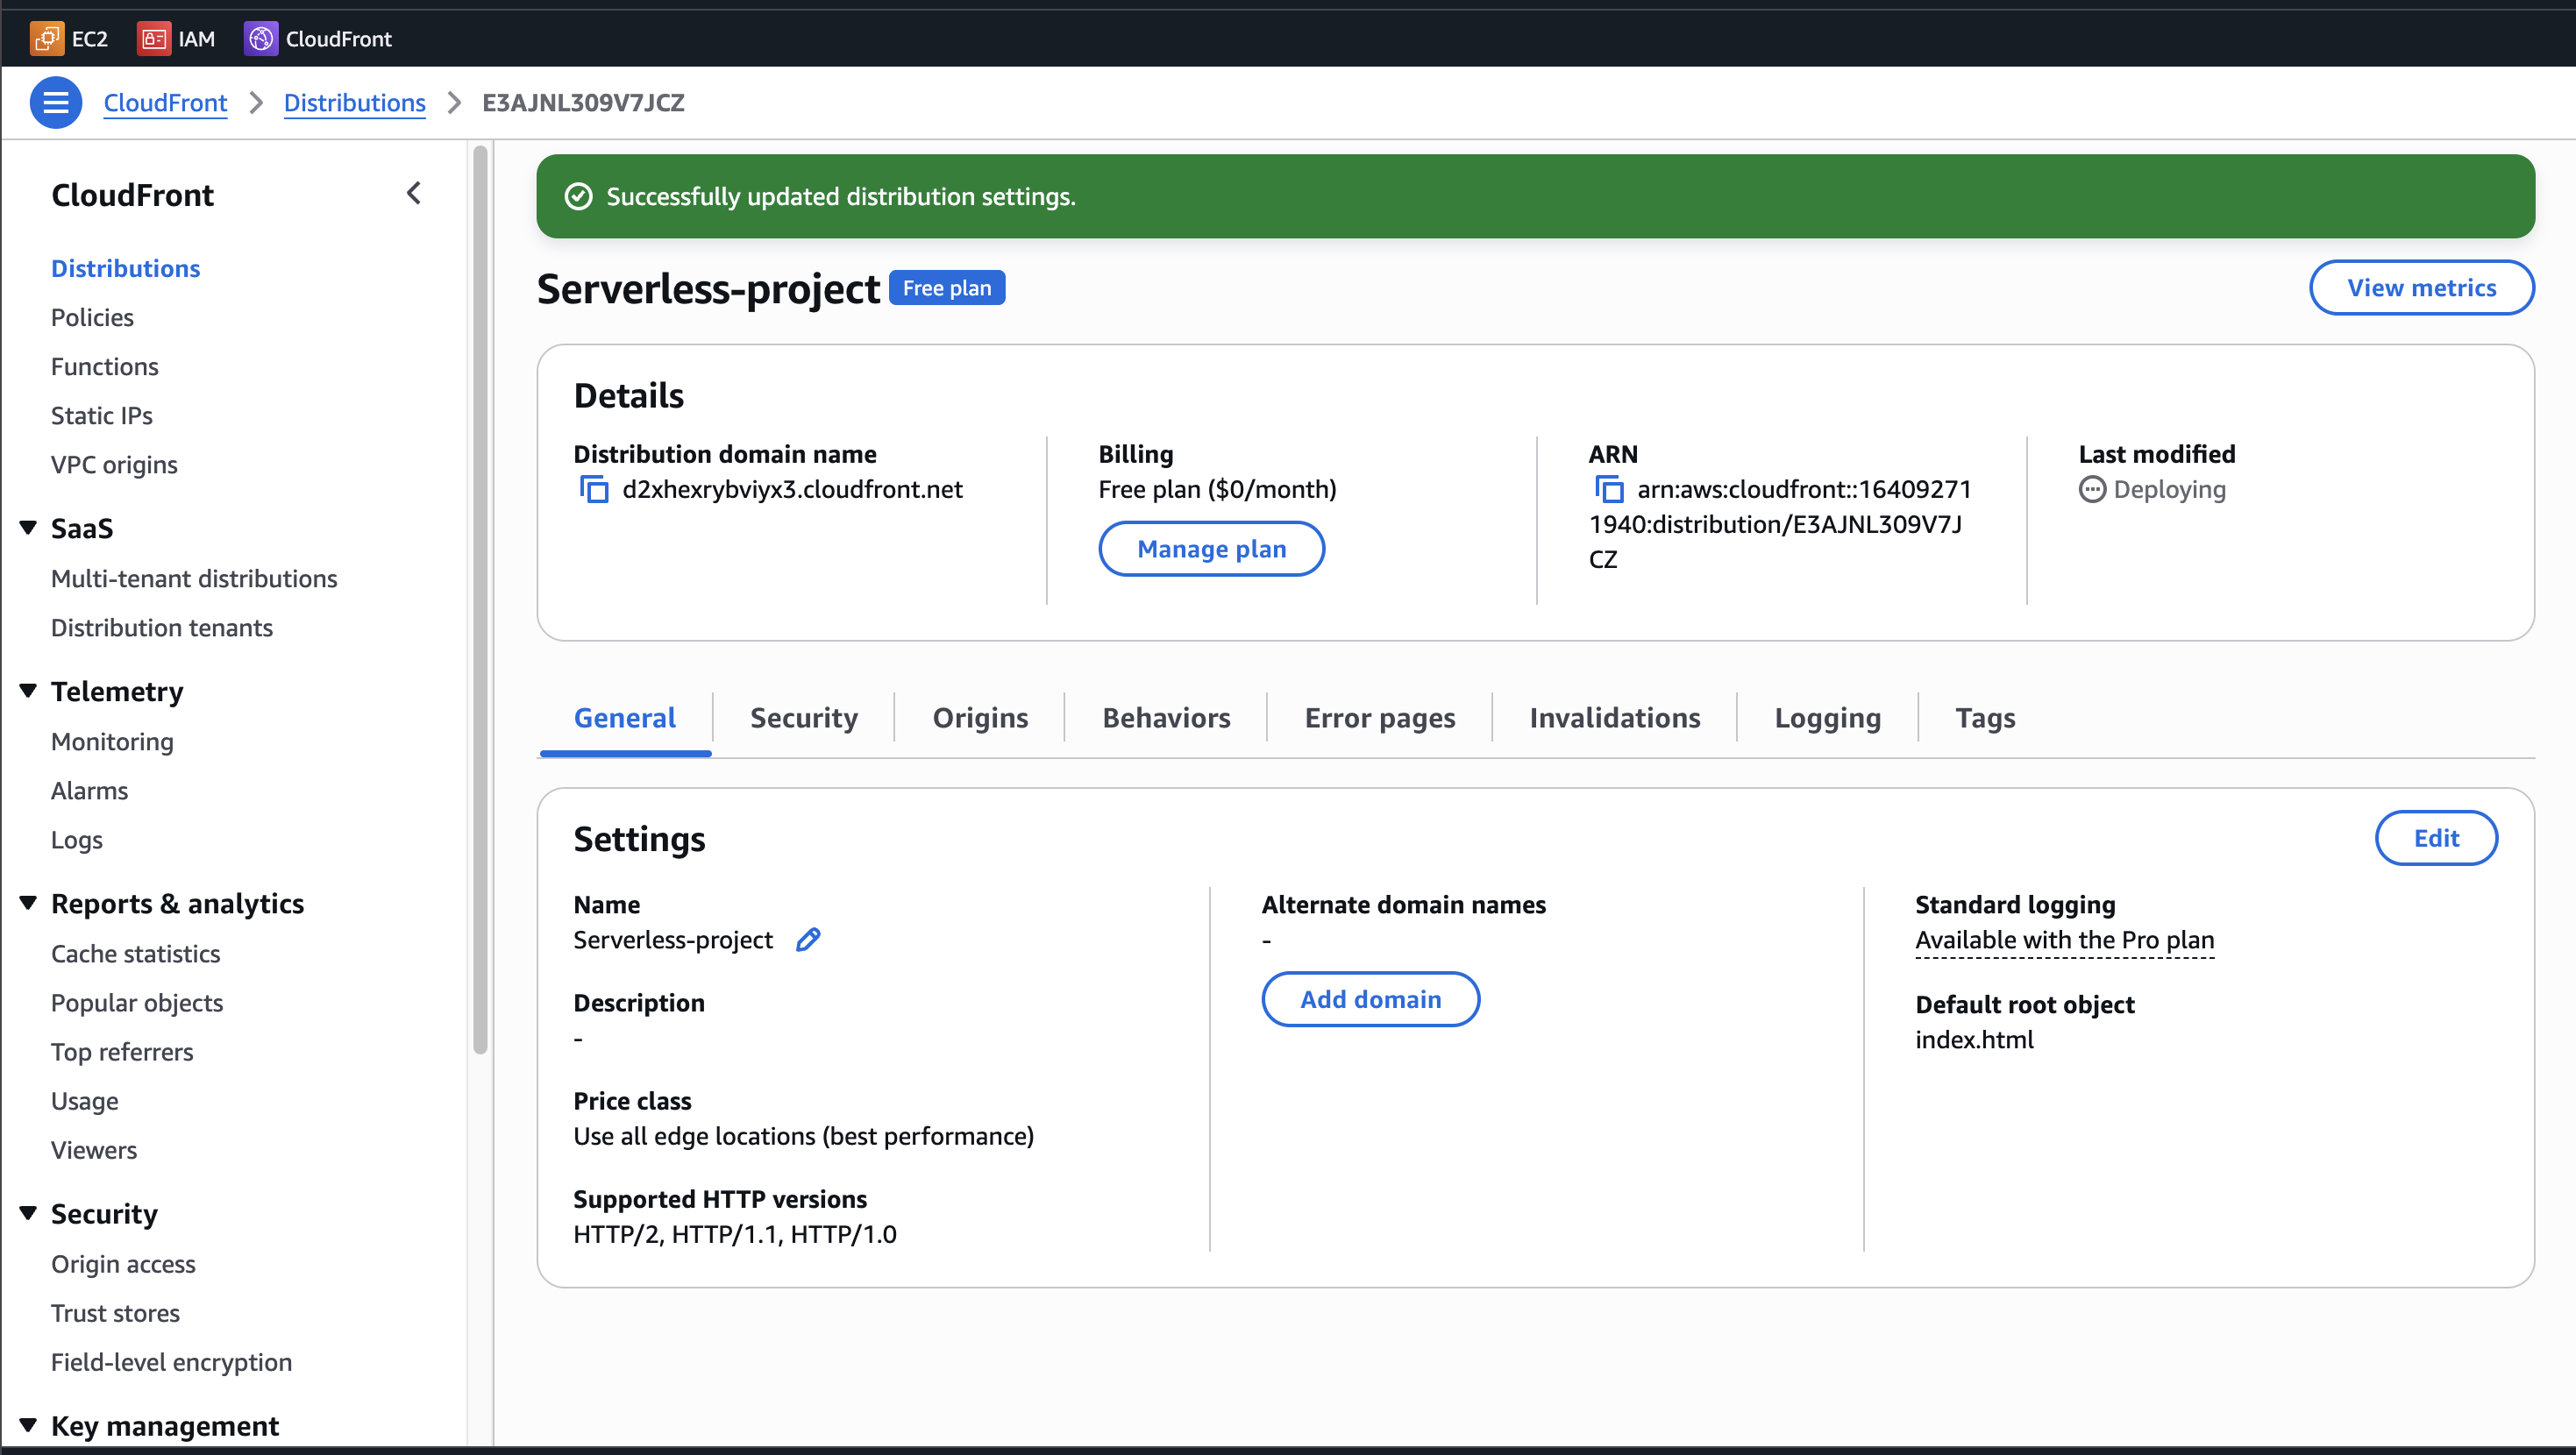
\includegraphics[width=0.9\textwidth]{img/SE-4_cloudfront_oac_2.png}
\caption{Chi tiết OAC configuration}
\label{fig:se4b}
\end{figure}

Origin Access Control settings:
\begin{itemize}
    \item Origin access: Origin access control settings (recommended)
    \item OAC name: task-manager-oac
    \item Signing behavior: Sign requests (recommended)
    \item Origin type: S3
\end{itemize}

\subsection{Networking Security Evidence}
\label{ssec:network_security}

\subsubsection{NE-1: VPC Endpoint Created for DynamoDB}

Hình \ref{fig:ne1} cho thấy VPC Gateway Endpoint cho DynamoDB đã được tạo thành công với status Available. Endpoint này cho phép Lambda kết nối DynamoDB qua mạng private của AWS.

\begin{figure}[H]
\centering
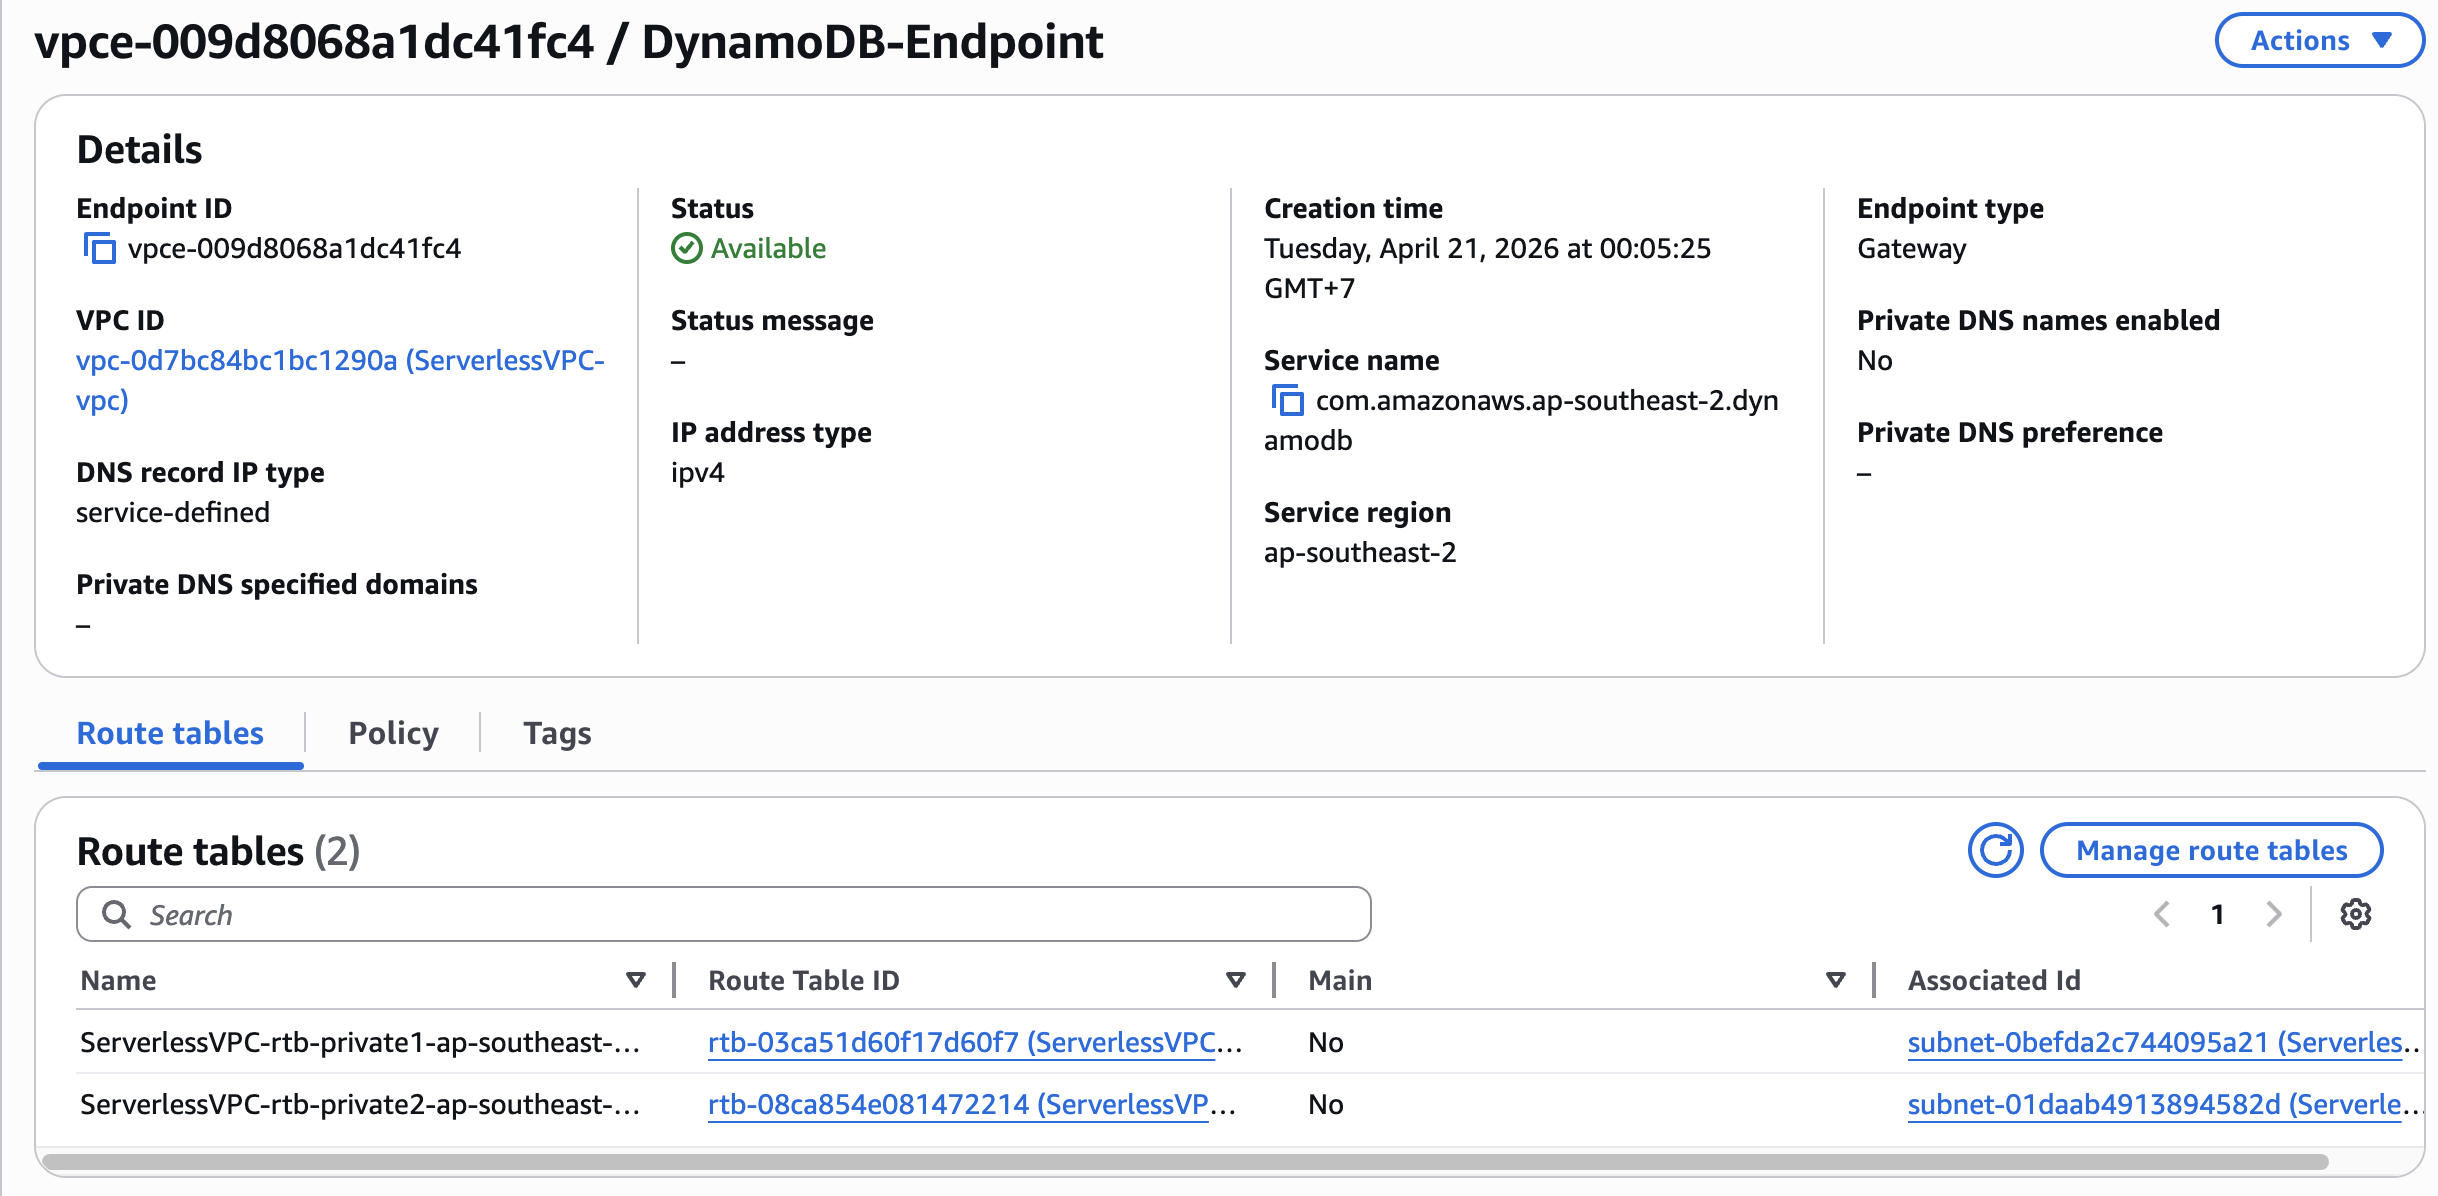
\includegraphics[width=0.9\textwidth]{img/NE-1_vpc_endpoint.png}
\caption{VPC Gateway Endpoint cho DynamoDB với status Available}
\label{fig:ne1}
\end{figure}

Thông tin endpoint:
\begin{itemize}
    \item Service name: com.amazonaws.ap-southeast-1.dynamodb
    \item Type: Gateway
    \item Status: Available
    \item VPC: Custom VPC (10.0.0.0/16)
    \item Route tables: Private Route Table
\end{itemize}

\subsubsection{NE-2: Lambda Has VpcConfig}

Hình \ref{fig:ne2} minh chứng Lambda function đã được attach vào VPC với cấu hình VpcConfig bao gồm subnets và security group.

\begin{figure}[H]
\centering
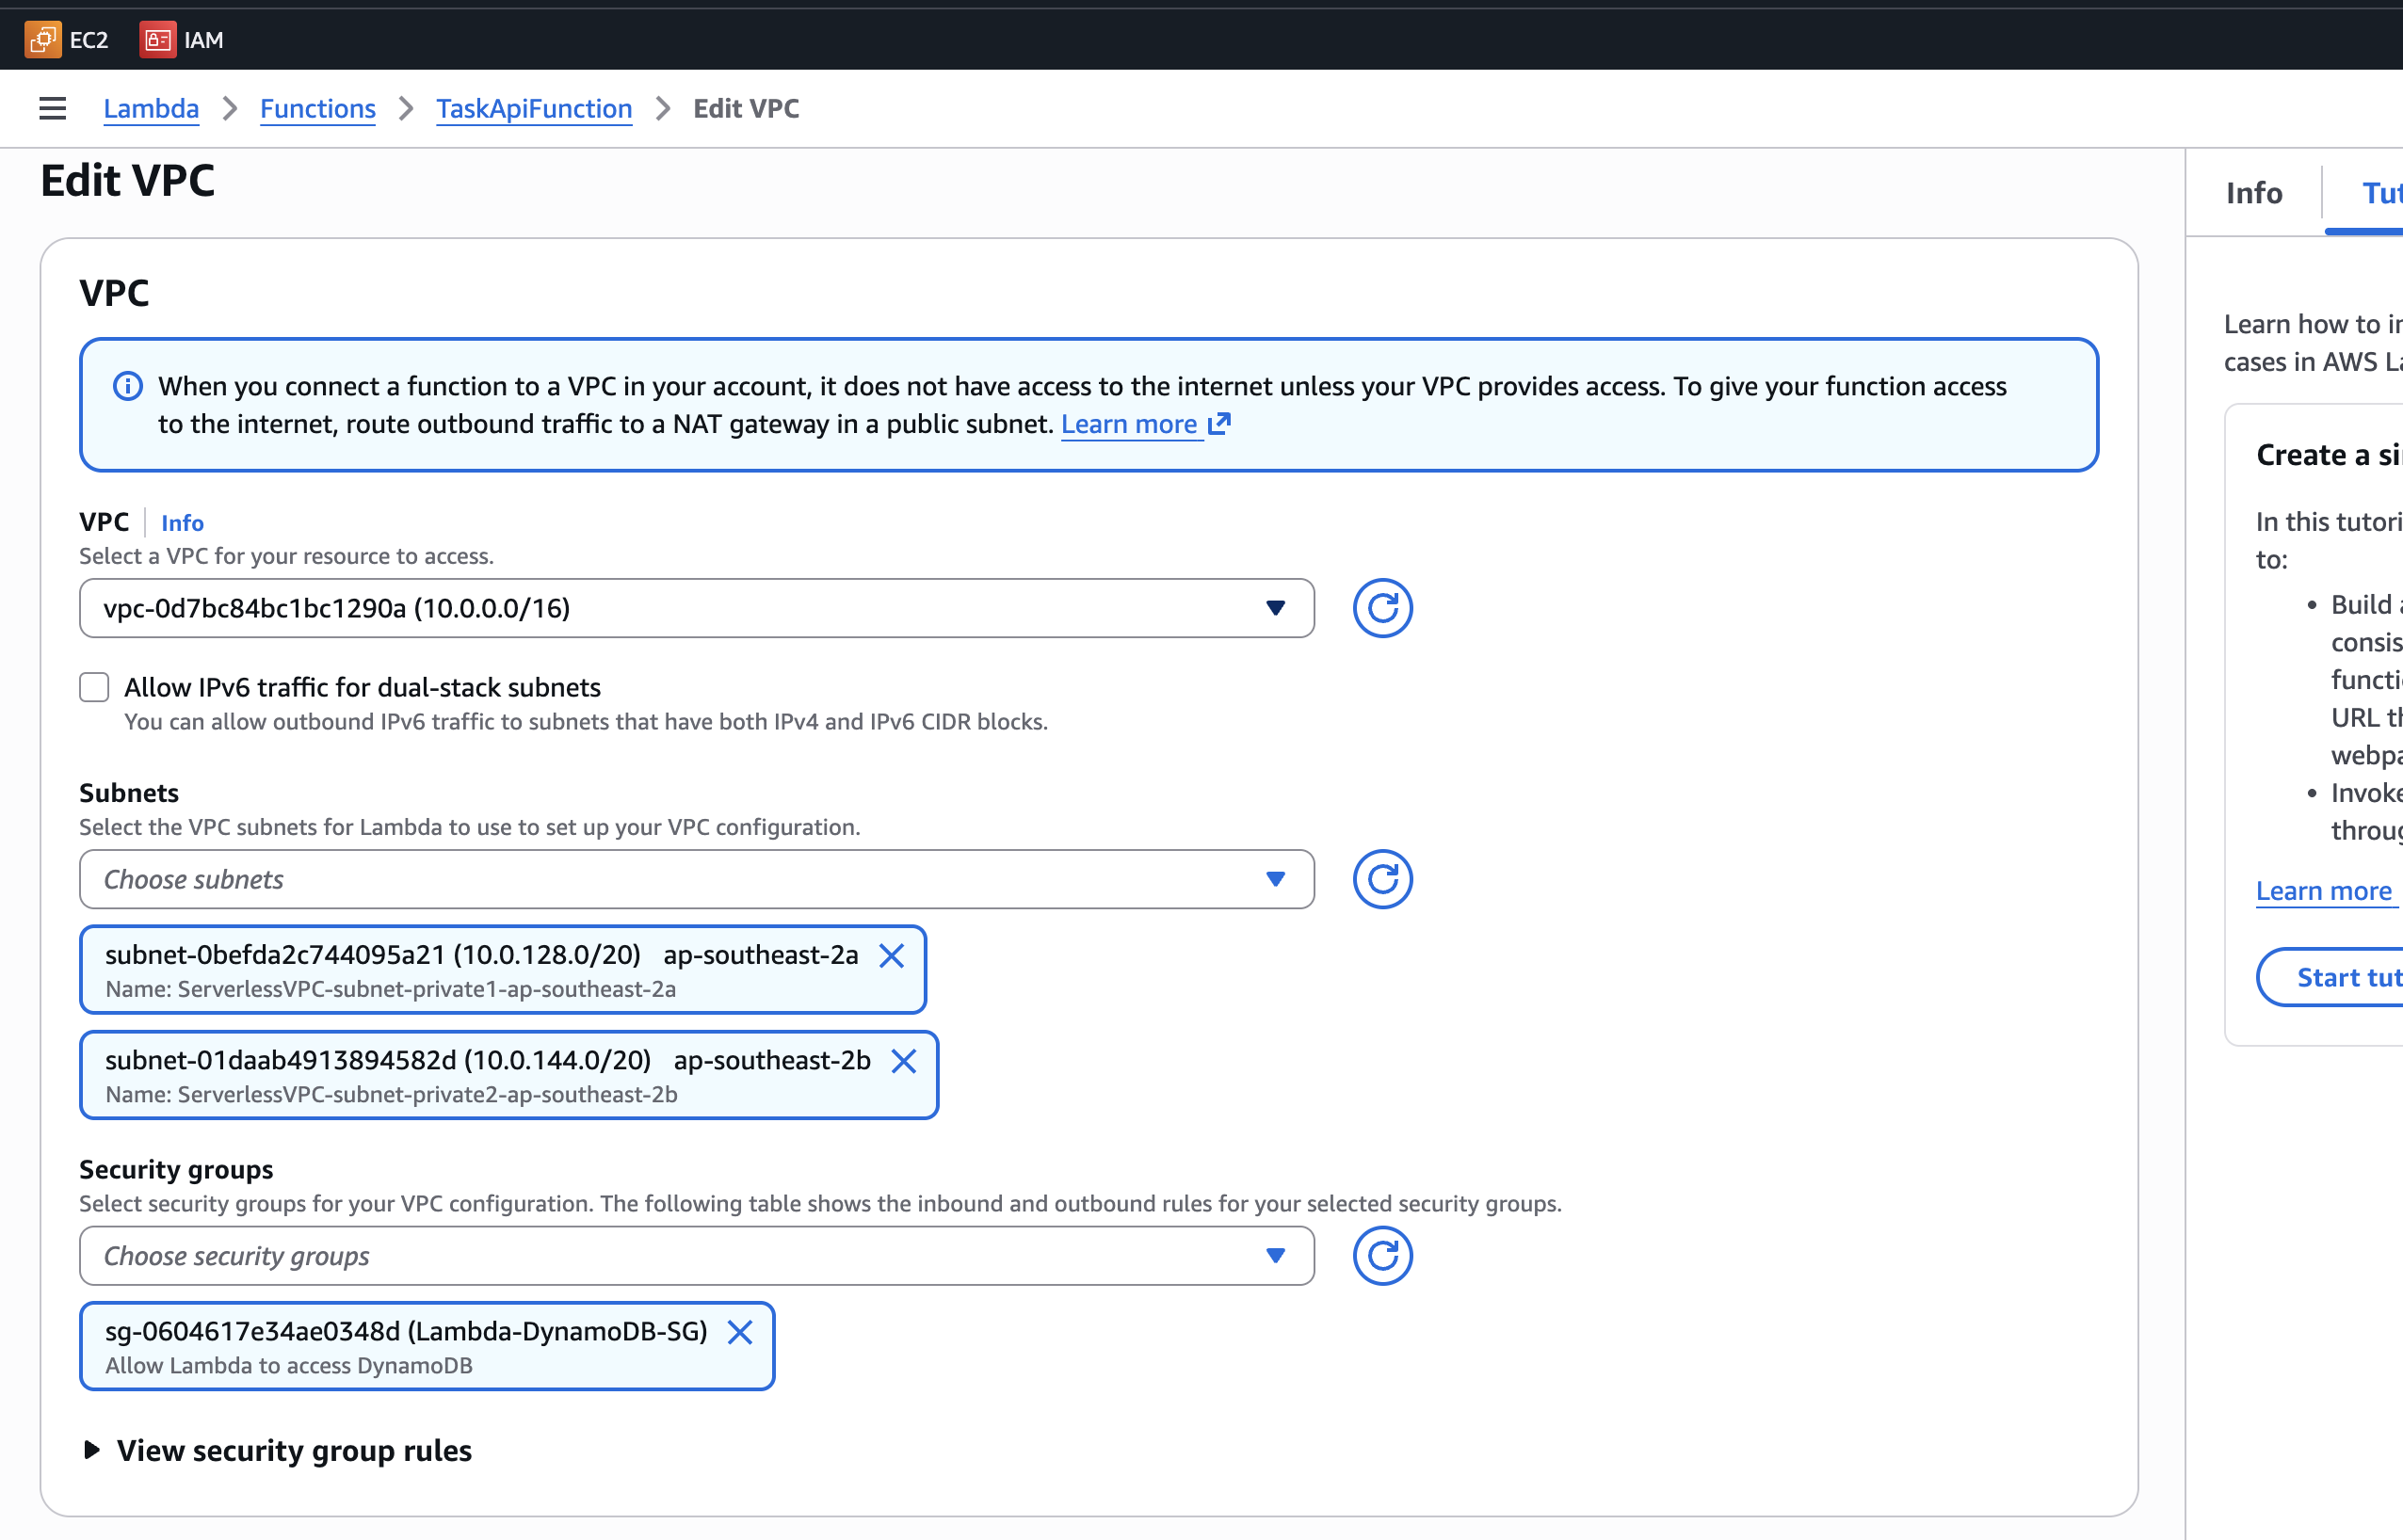
\includegraphics[width=0.9\textwidth]{img/NE-2_lambda_vpc_config.png}
\caption{Lambda VPC Configuration với subnets và security group}
\label{fig:ne2}
\end{figure}

VPC Configuration:
\begin{itemize}
    \item VPC: Custom VPC
    \item Subnets: Private Subnet A (10.0.1.0/24), Private Subnet B (10.0.2.0/24)
    \item Security groups: lambda-sg
    \item Network interfaces: ENI được tạo tự động trong các subnets
\end{itemize}

\subsubsection{NE-3: Route Table Has Endpoint Route}

Hình \ref{fig:ne3} hiển thị Private Route Table với route entry trỏ đến VPC Endpoint. Route này đảm bảo traffic đến DynamoDB đi qua endpoint thay vì Internet.

\begin{figure}[H]
\centering
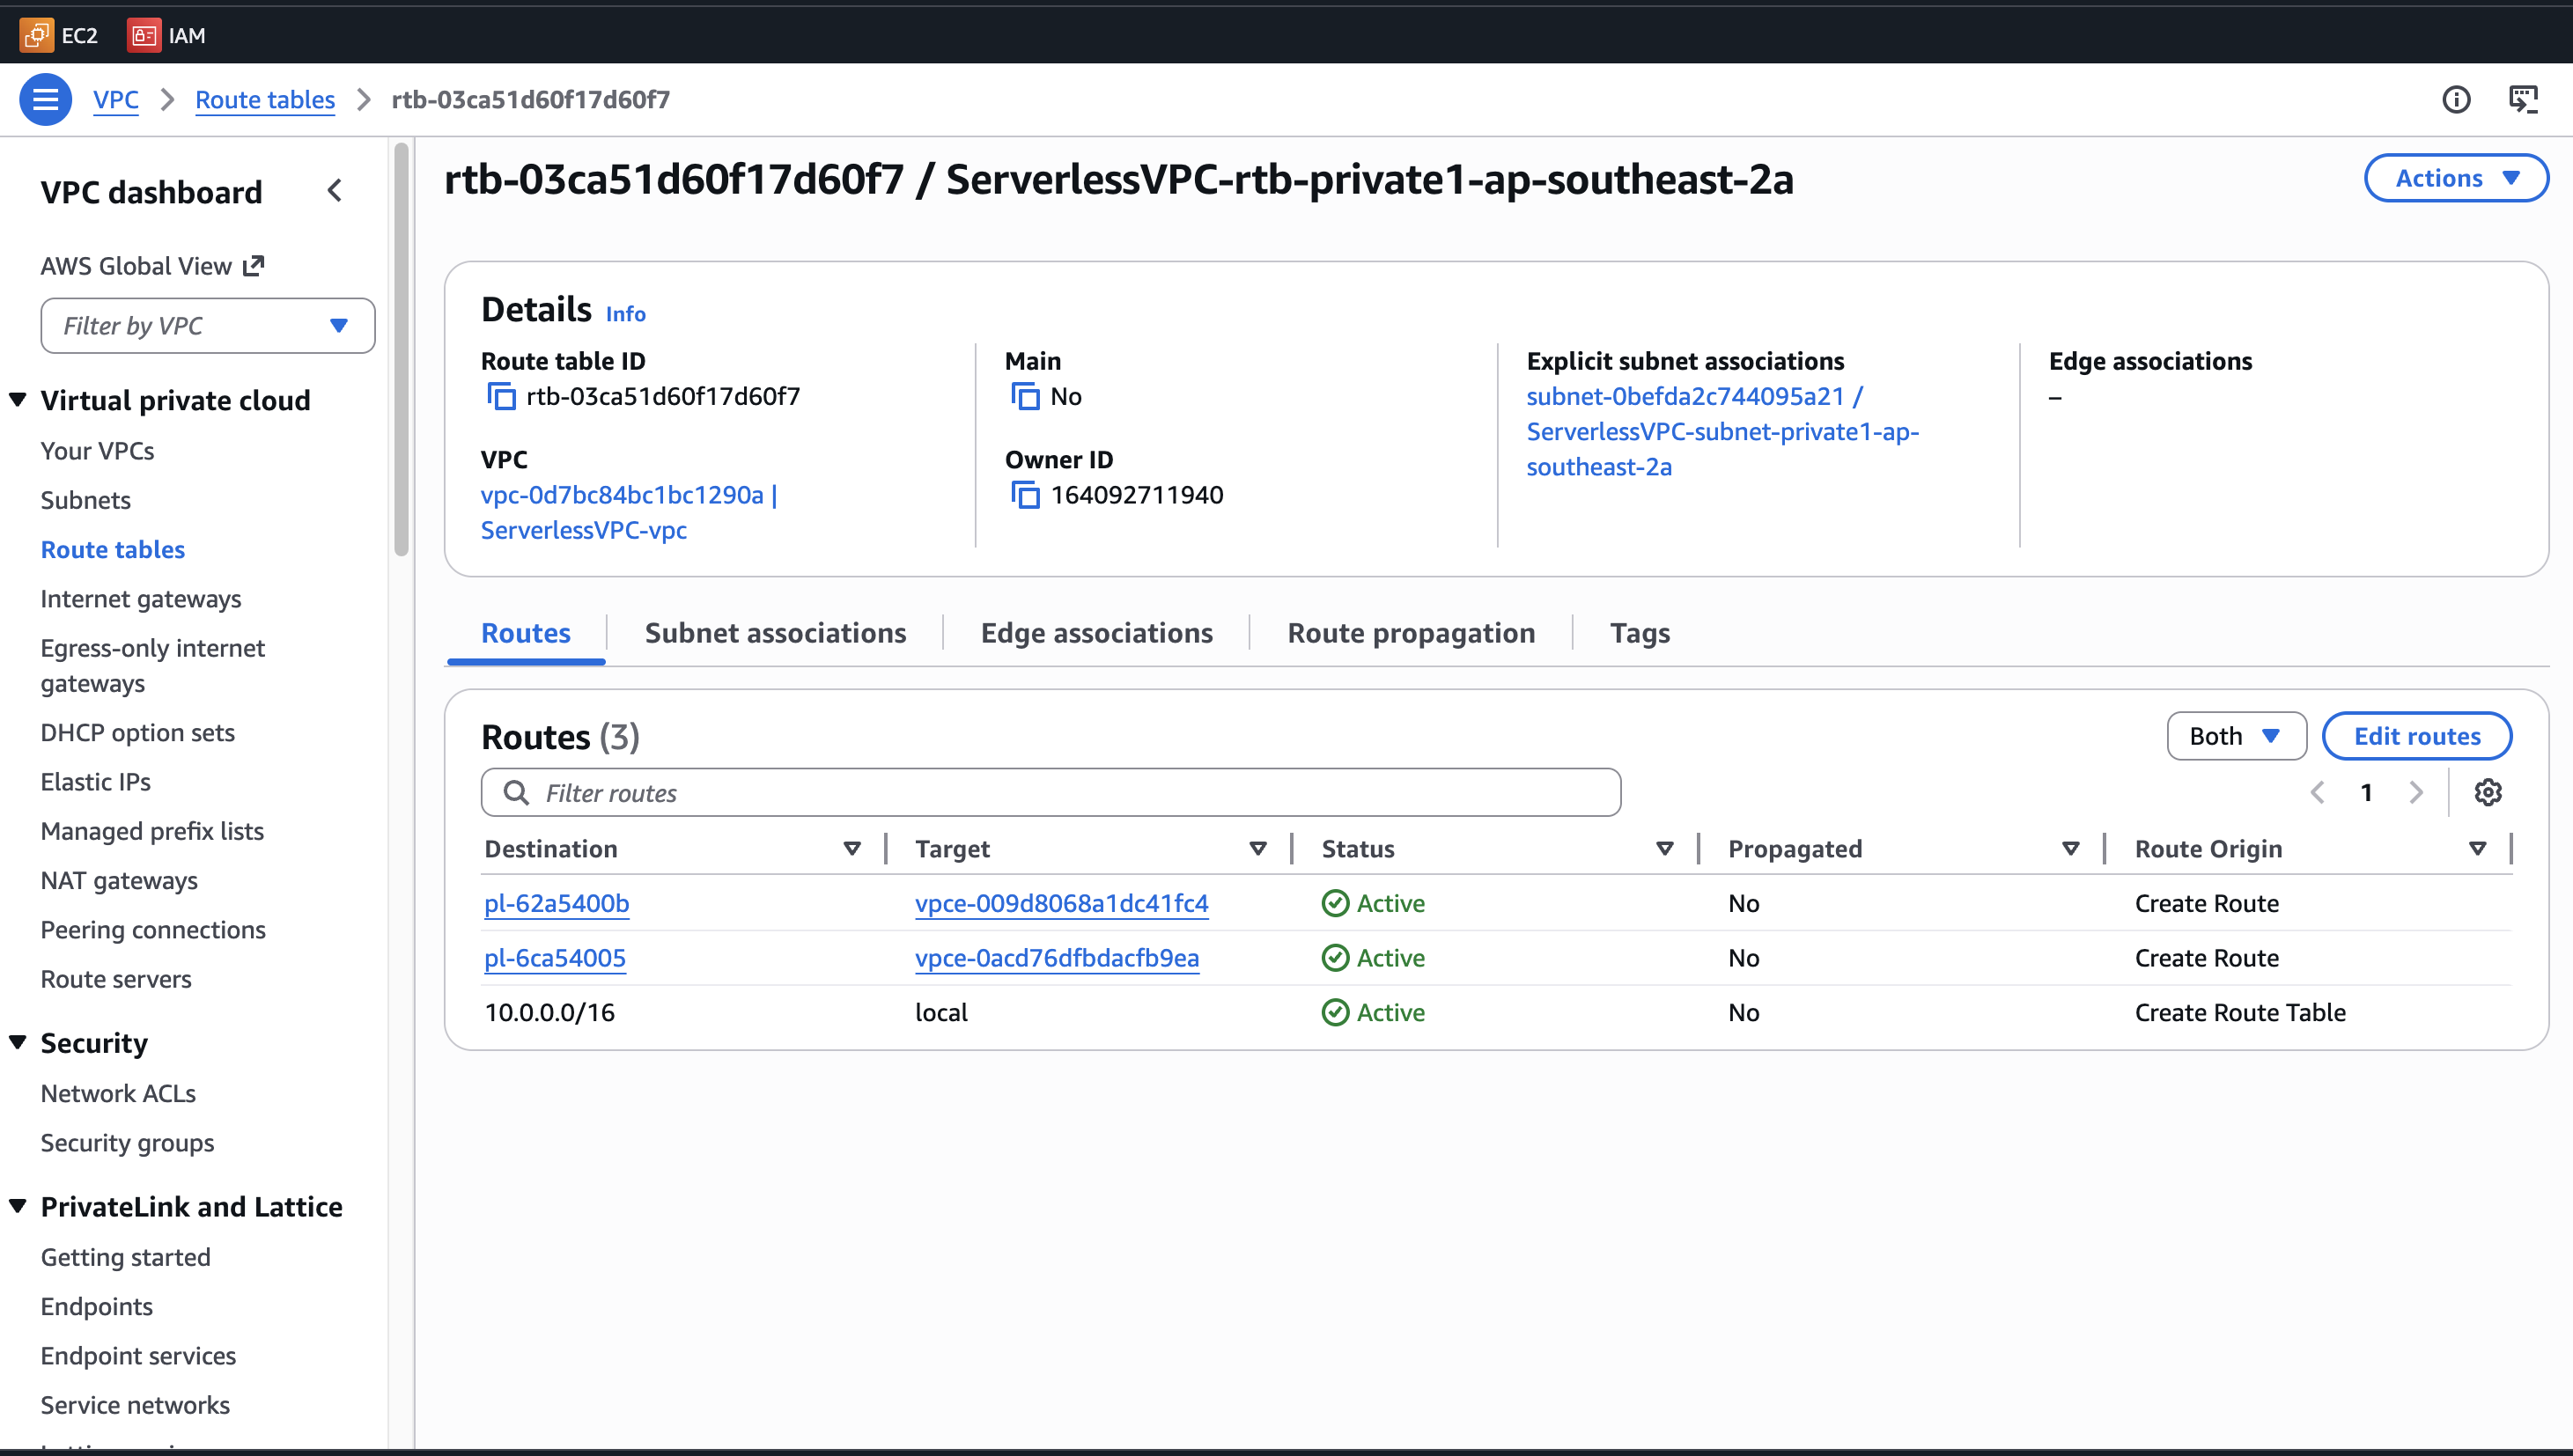
\includegraphics[width=0.9\textwidth]{img/NE-3_route_table.png}
\caption{Route Table với entry pl-xxxxx → vpce-xxxxx}
\label{fig:ne3}
\end{figure}

Route entries:
\begin{itemize}
    \item Destination: 10.0.0.0/16 → Target: local (VPC internal routing)
    \item Destination: pl-xxxxx (DynamoDB Prefix List) → Target: vpce-xxxxx (VPC Endpoint)
\end{itemize}

\subsubsection{NE-4: No NAT Gateway Exists}

Hình \ref{fig:ne4} xác nhận không có NAT Gateway nào tồn tại trong VPC. Điều này quan trọng để đảm bảo chi phí bằng 0 (NAT Gateway tốn ~\$32/month).

\begin{figure}[H]
\centering
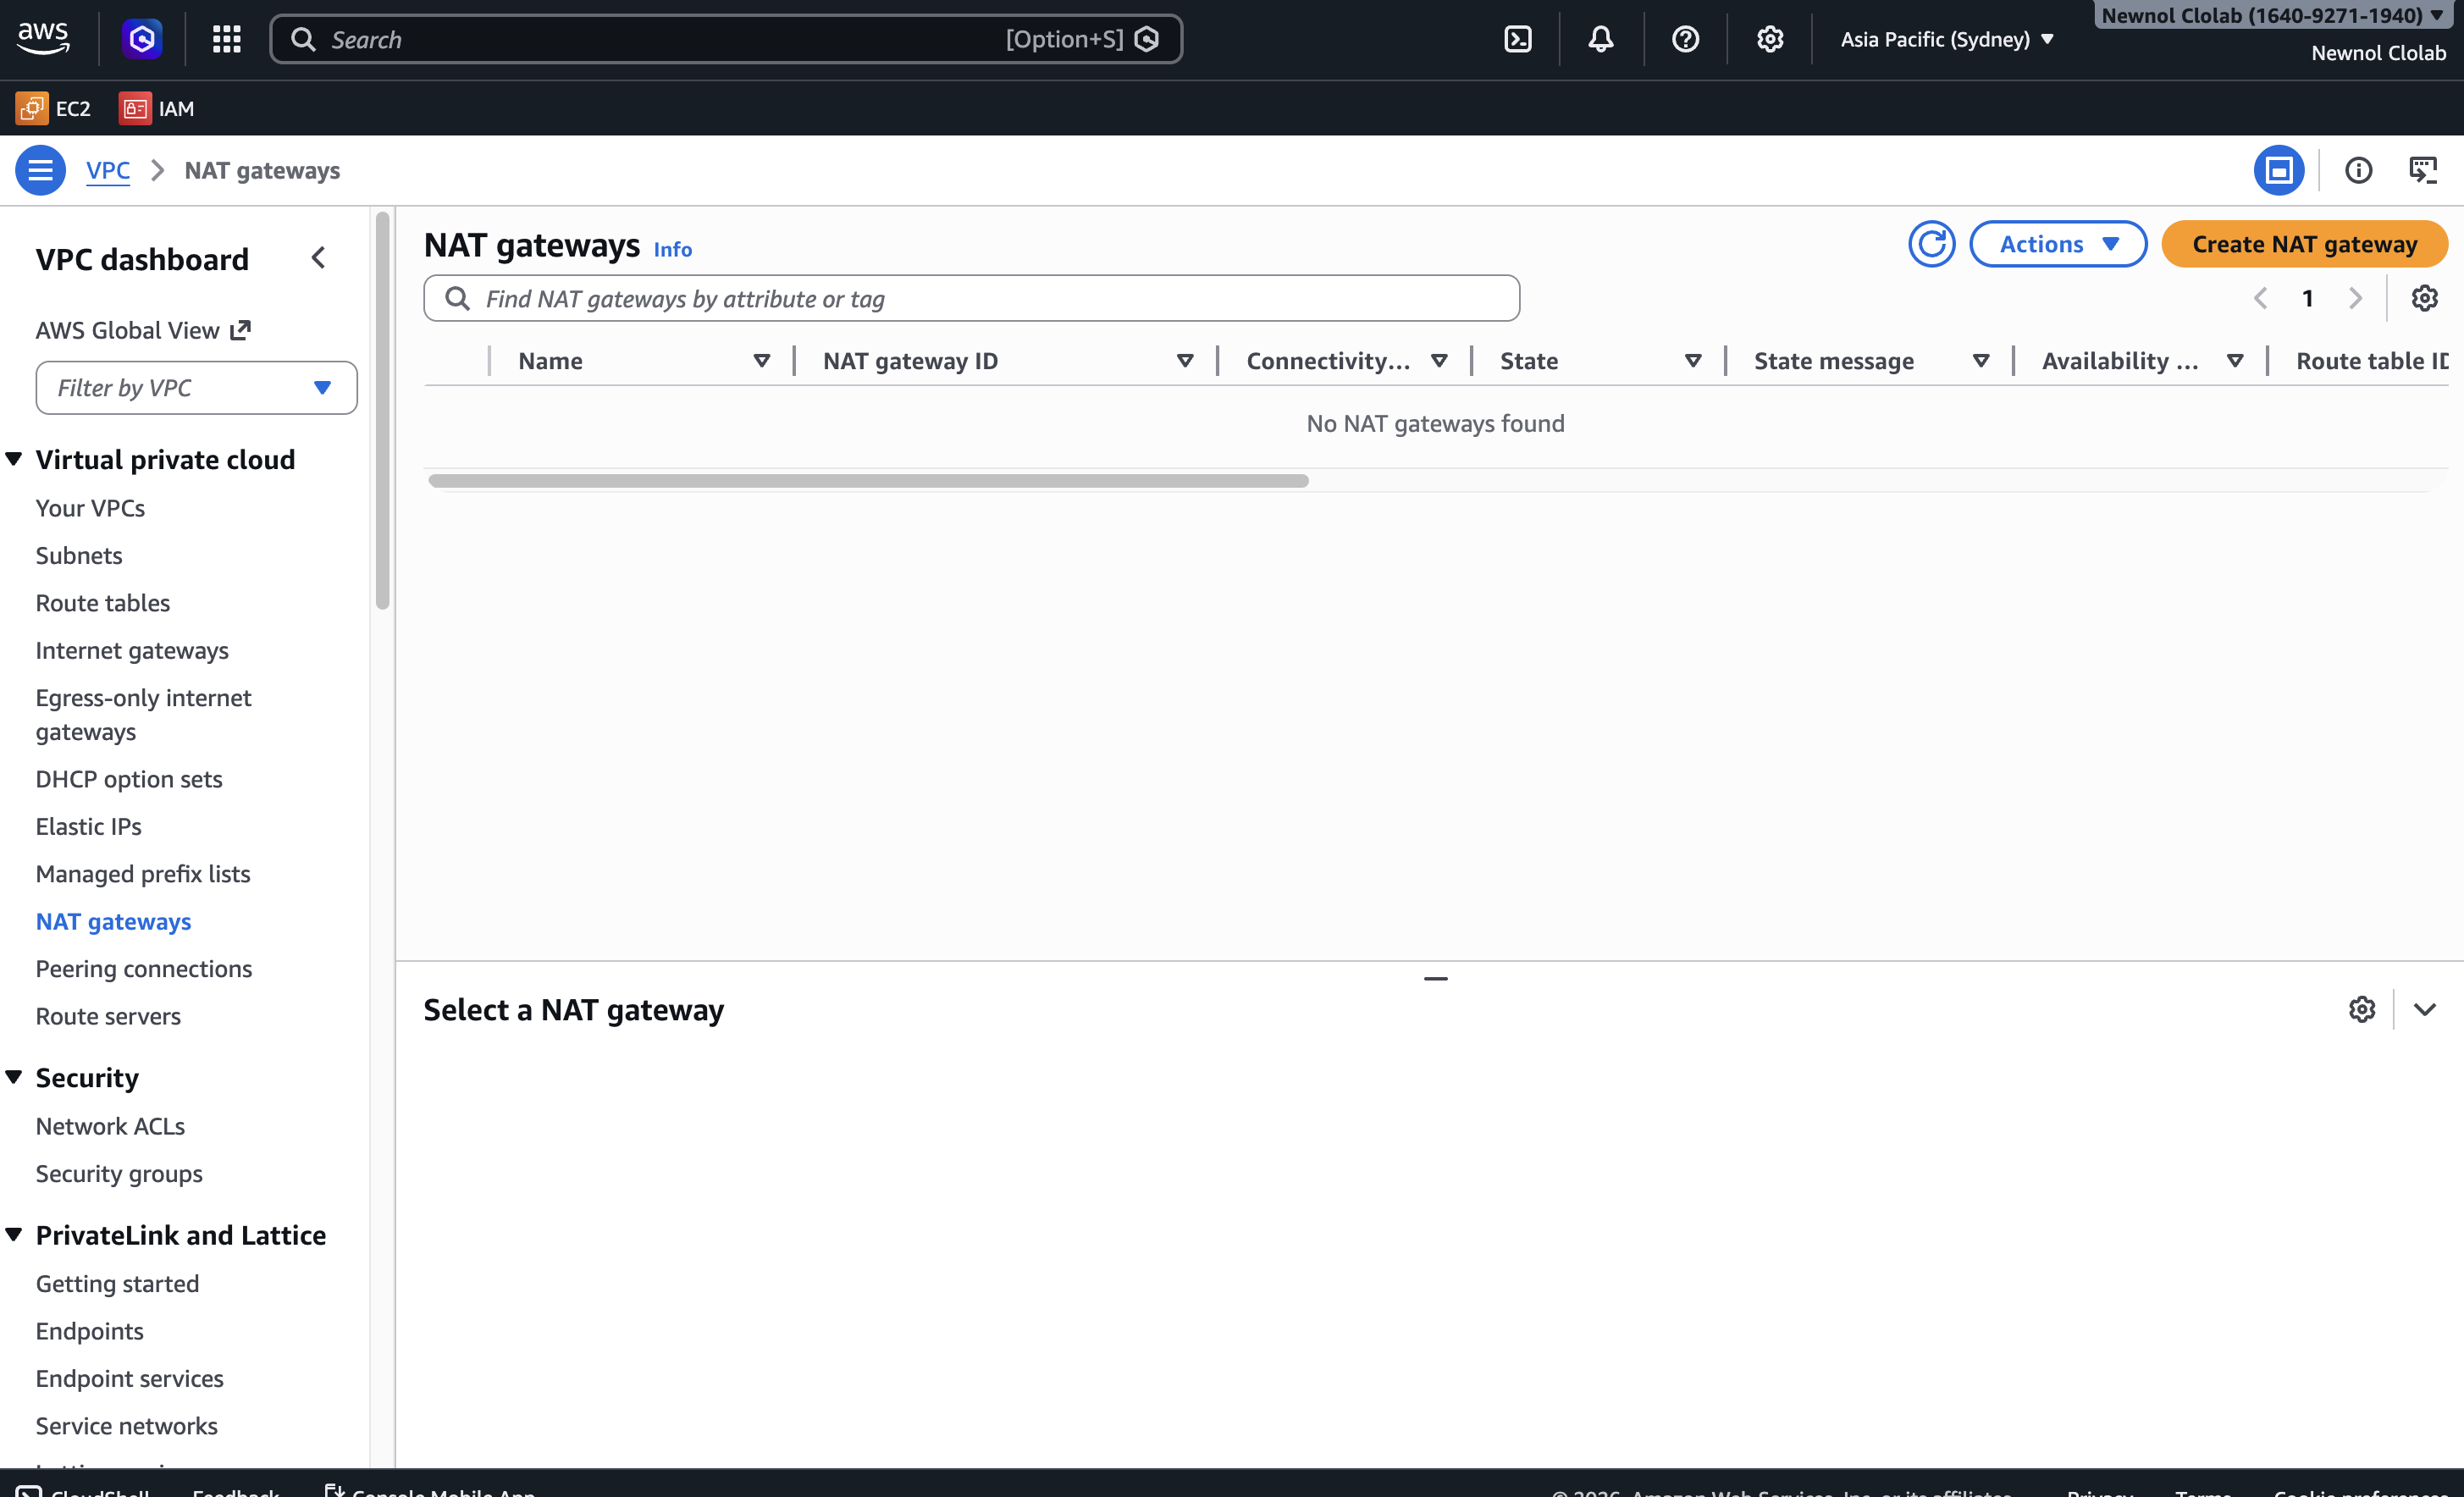
\includegraphics[width=0.9\textwidth]{img/NE-4_no_nat_gateway.png}
\caption{Danh sách NAT Gateways trống - không có NAT Gateway}
\label{fig:ne4}
\end{figure}

\subsubsection{NE-5: Lambda Successfully Calls DynamoDB}

Hình \ref{fig:ne5} cho thấy CloudWatch log của Lambda invocation thành công, với DynamoDB call trả về status code 200. Điều này chứng minh kết nối private qua VPC Endpoint hoạt động đúng.

\begin{figure}[H]
\centering
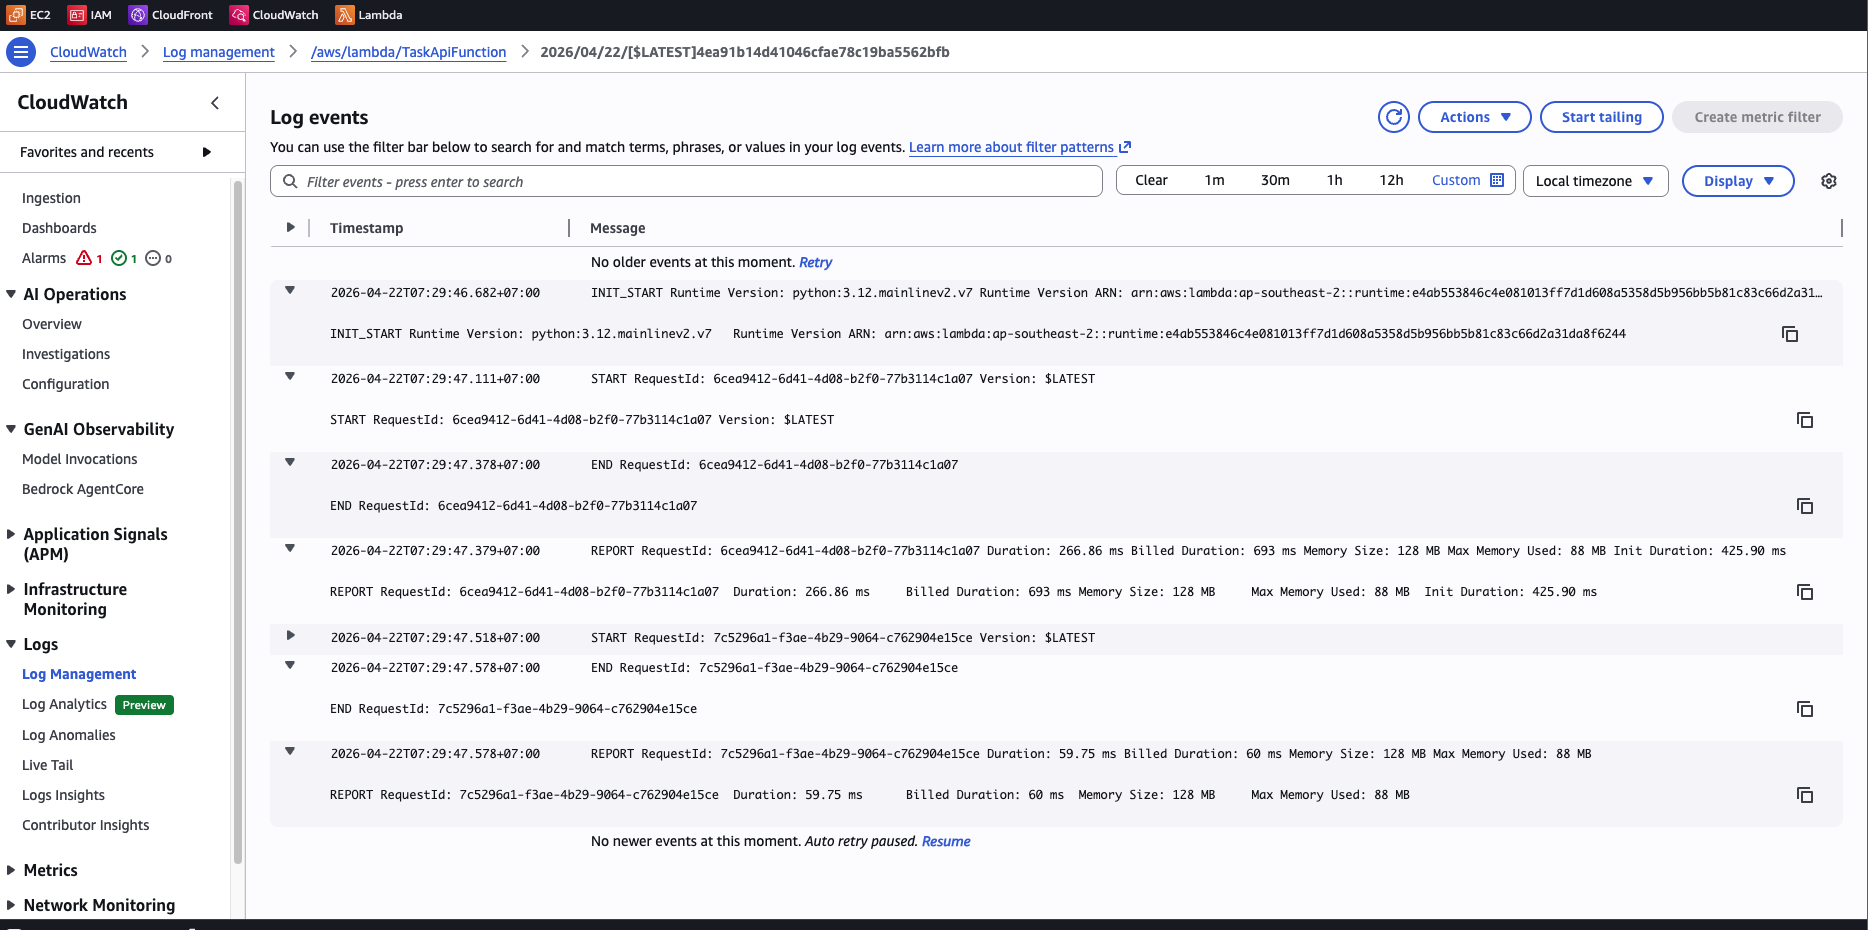
\includegraphics[width=0.9\textwidth]{img/NE-5.png}
\caption{CloudWatch log - Lambda gọi DynamoDB thành công qua VPC Endpoint}
\label{fig:ne5}
\end{figure}

Log details:
\begin{itemize}
    \item Request ID: xxxxx-xxxxx-xxxxx
    \item Duration: ~200ms
    \item Billed Duration: 300ms
    \item Memory Used: 128 MB
    \item DynamoDB response: StatusCode 200
    \item No NetworkingError hoặc UnauthorizedAccess error
\end{itemize}

\subsection{IAM Security Evidence}
\label{ssec:iam_security}

\subsubsection{IM-1: Two Separate IAM Roles}

Hình \ref{fig:im1} hiển thị hai IAM Roles riêng biệt đã được tạo cho các Lambda functions khác nhau, tuân thủ nguyên tắc Least Privilege.

\begin{figure}[H]
\centering
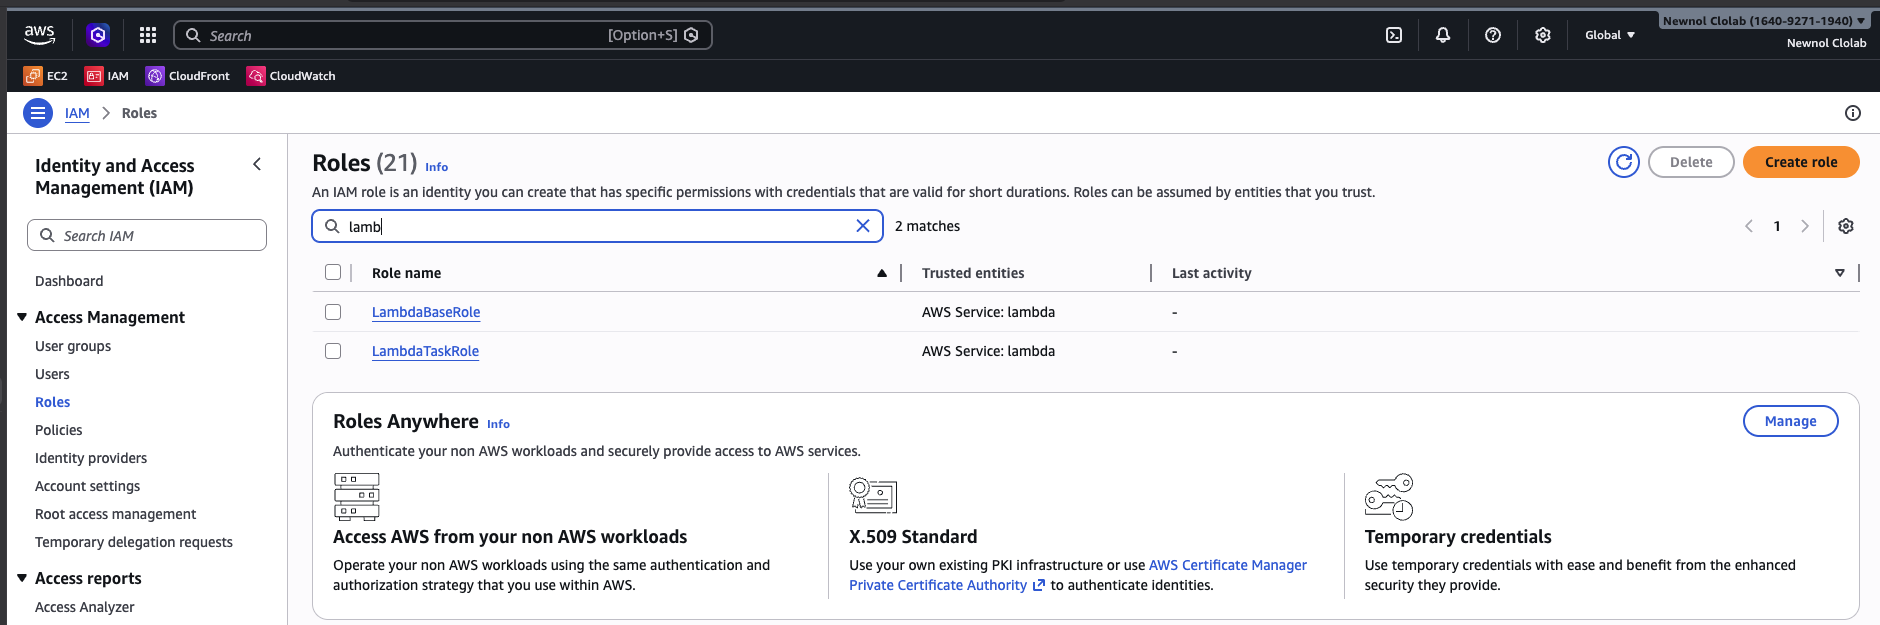
\includegraphics[width=0.9\textwidth]{img/IM-1_IAM_role.png}
\caption{Hai IAM Roles riêng biệt: LambdaTaskRole và LambdaBaseRole}
\label{fig:im1}
\end{figure}

Roles:
\begin{itemize}
    \item \textbf{LambdaTaskRole:} Cho Lambda xử lý tasks - có quyền DynamoDB + CloudWatch Logs + ENI
    \item \textbf{LambdaBaseRole:} Cho Lambda khác - chỉ có CloudWatch Logs + ENI
\end{itemize}

\subsubsection{IM-2: Policy Specifies Exact Resource ARN}

Hình \ref{fig:im2a} và \ref{fig:im2b} cho thấy IAM Policy JSON với Resource field chỉ định chính xác DynamoDB table ARN, không sử dụng wildcard (*).

\begin{figure}[H]
\centering
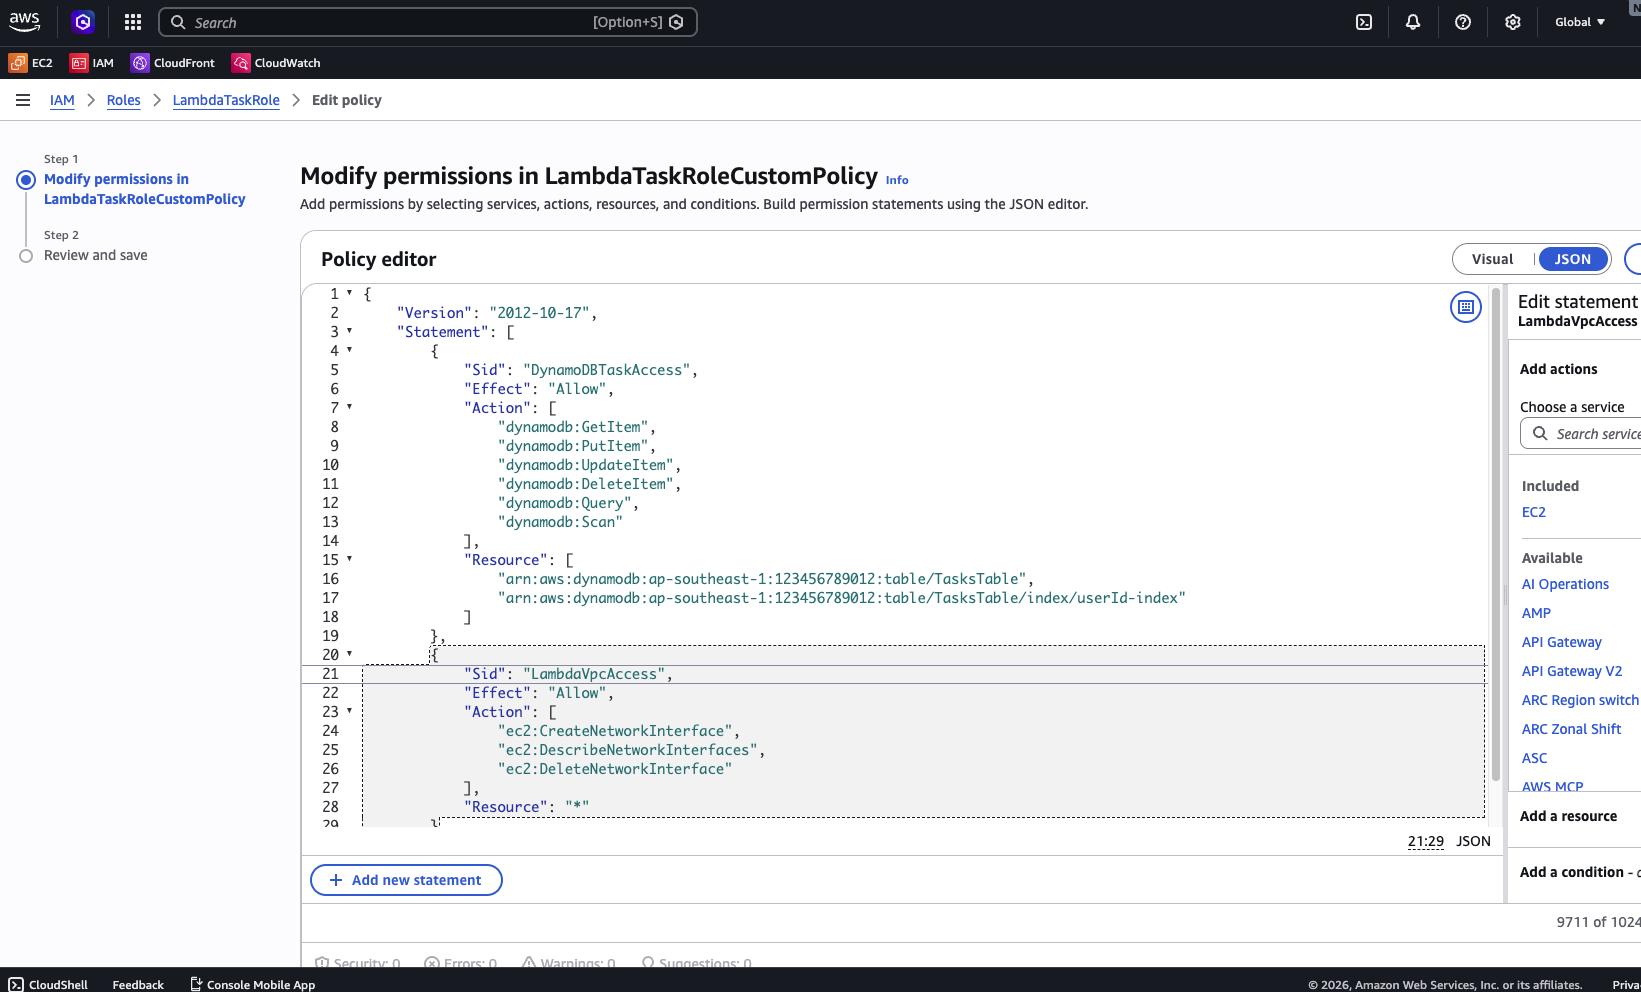
\includegraphics[width=0.9\textwidth]{img/IM-2_LambdaTaskRole.png}
\caption{LambdaTaskRole Policy với specific DynamoDB table ARN}
\label{fig:im2a}
\end{figure}

\begin{figure}[H]
\centering
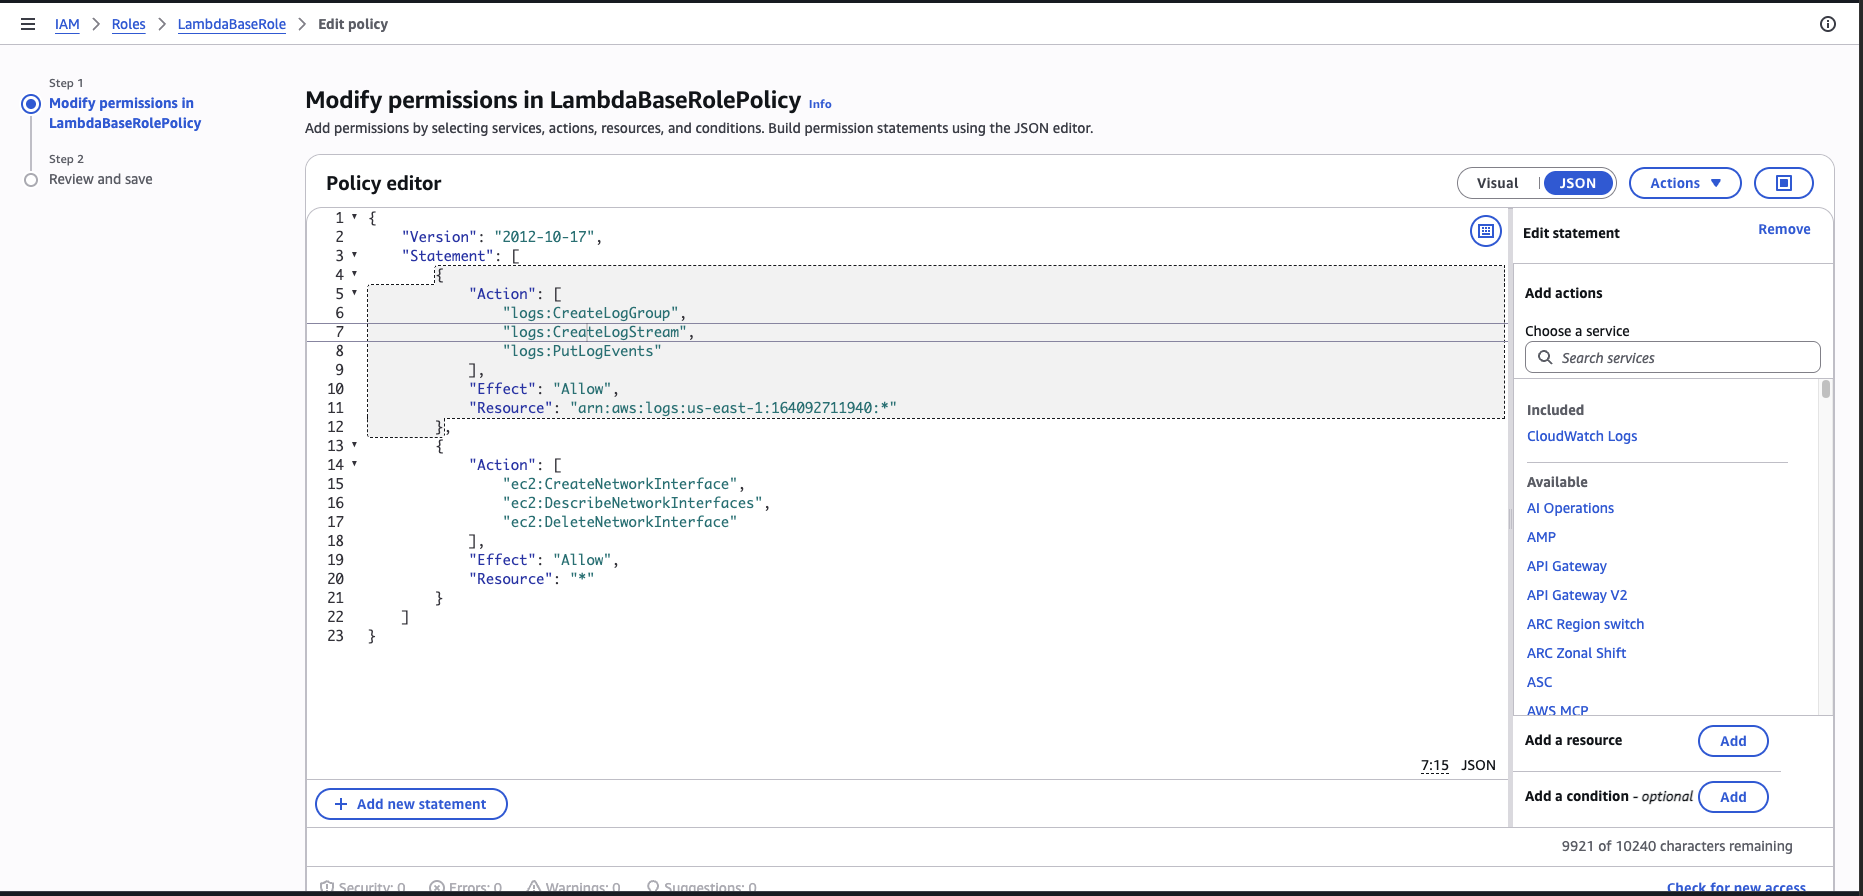
\includegraphics[width=0.9\textwidth]{img/IM-2_LambdaBaseRole.png}
\caption{LambdaBaseRole Policy - không có DynamoDB permissions}
\label{fig:im2b}
\end{figure}

Policy highlights:
\begin{itemize}
    \item Resource: "arn:aws:dynamodb:ap-southeast-1:123456789012:table/Tasks"
    \item Resource: "arn:aws:dynamodb:ap-southeast-1:123456789012:table/Tasks/index/*"
    \item Không có wildcard "*" cho DynamoDB resources
\end{itemize}

\subsubsection{IM-3: Lambda Attached to Correct Role}

Hình \ref{fig:im3} xác nhận Lambda function đã được attach đúng IAM Role với permissions phù hợp.

\begin{figure}[H]
\centering
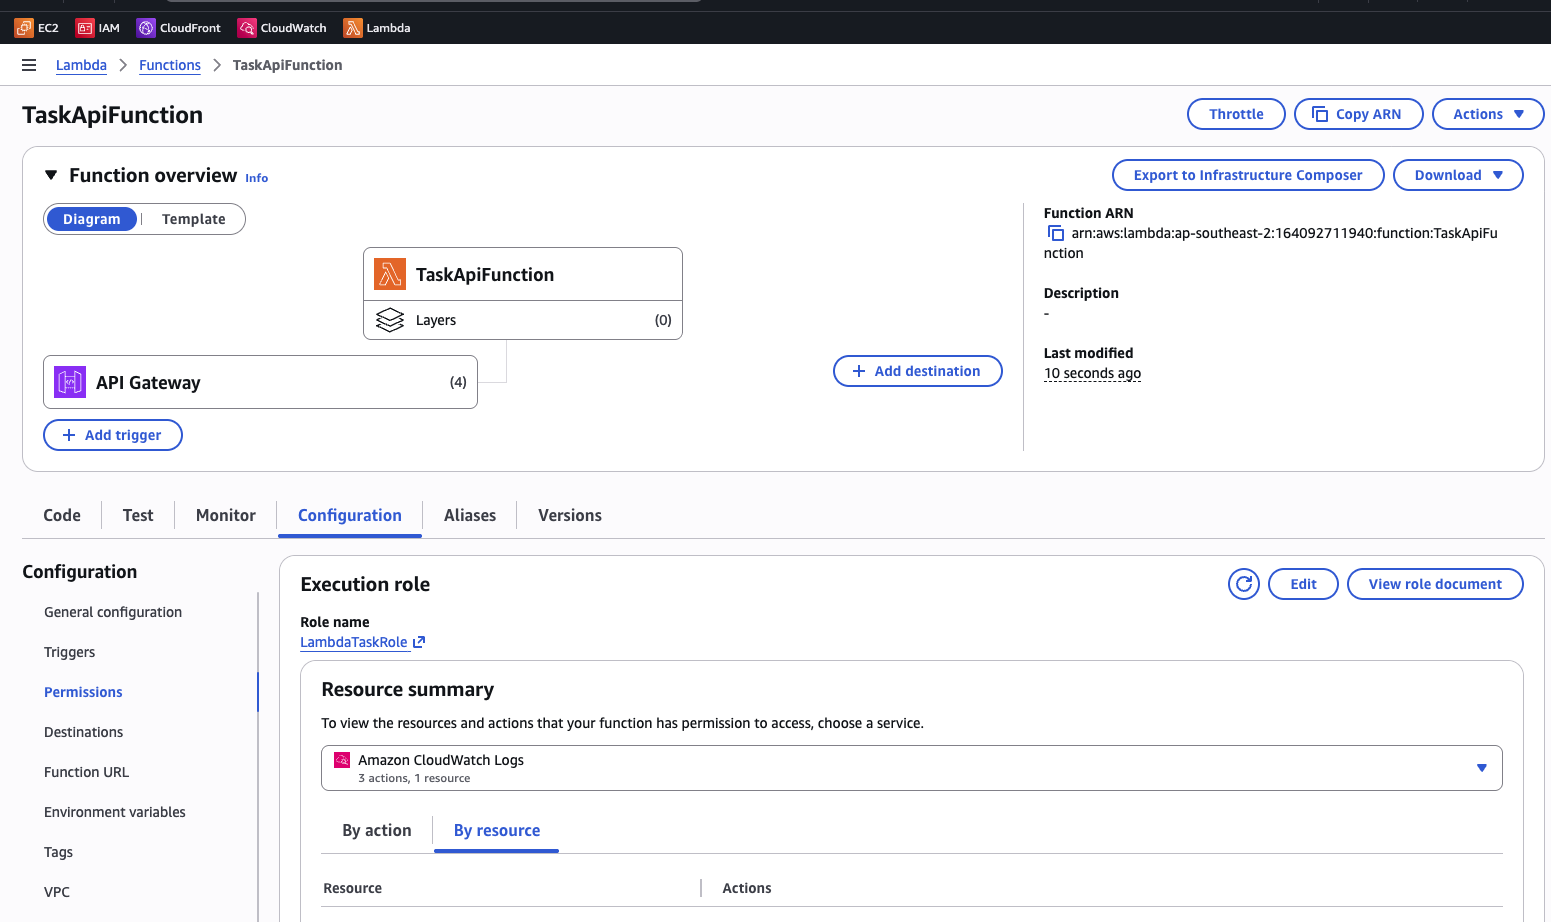
\includegraphics[width=0.9\textwidth]{img/IM-3_TaskApiFunction.png}
\caption{Lambda Configuration - Execution role: LambdaTaskRole}
\label{fig:im3}
\end{figure}

\subsection{Tổng kết bảo mật}
\label{ssec:security_summary}

Hệ thống đã triển khai đầy đủ các biện pháp bảo mật theo yêu cầu:

\begin{table}[H]
\centering
\begin{tabular}{|l|l|c|}
\hline
\textbf{ID} & \textbf{Evidence Item} & \textbf{Status} \\
\hline
SE-1 & S3 Block Public Access enabled & ✓ \\
SE-2 & Direct S3 access rejected (403) & ✓ \\
SE-3 & CloudFront access succeeds (200) & ✓ \\
SE-4 & OAC attached to CloudFront & ✓ \\
NE-1 & VPC Endpoint for DynamoDB & ✓ \\
NE-2 & Lambda VpcConfig attached & ✓ \\
NE-3 & Route Table has endpoint route & ✓ \\
NE-4 & No NAT Gateway exists & ✓ \\
NE-5 & Lambda calls DynamoDB successfully & ✓ \\
IM-1 & Two separate IAM Roles & ✓ \\
IM-2 & Policy with specific ARN & ✓ \\
IM-3 & Lambda attached to correct Role & ✓ \\
\hline
\end{tabular}
\caption{Checklist bằng chứng bảo mật}
\label{tab:security_checklist}
\end{table}

\section{Giám sát và kiểm soát chi phí}
\label{sec:monitoring}

\subsection{CloudWatch Dashboard}
\label{ssec:cloudwatch_dashboard}

CloudWatch Dashboard cung cấp cái nhìn tổng quan về hoạt động của hệ thống thông qua các metrics quan trọng.

\subsubsection{Dashboard Configuration}

Dashboard được đặt tên "TaskManager-Dashboard" và bao gồm các widgets sau:

\begin{enumerate}
    \item \textbf{Lambda Invocations:} Hiển thị tổng số lần Lambda được gọi, giúp theo dõi traffic pattern.
    
    \item \textbf{Lambda Duration:} Hiển thị P50 và P99 percentile của thời gian thực thi Lambda, giúp phát hiện performance issues.
    
    \item \textbf{Lambda Errors:} Số lượng errors xảy ra trong Lambda function, quan trọng để phát hiện bugs.
    
    \item \textbf{Lambda Throttles:} Số lần Lambda bị throttle do vượt quá Reserved Concurrency limit.
    
    \item \textbf{API Gateway Latency:} End-to-end response time từ API Gateway, bao gồm cả Lambda execution time.
    
    \item \textbf{API Gateway 4XX/5XX Errors:} Client errors (4XX) và server errors (5XX) từ API Gateway.
\end{enumerate}

\begin{figure}[H]
\centering
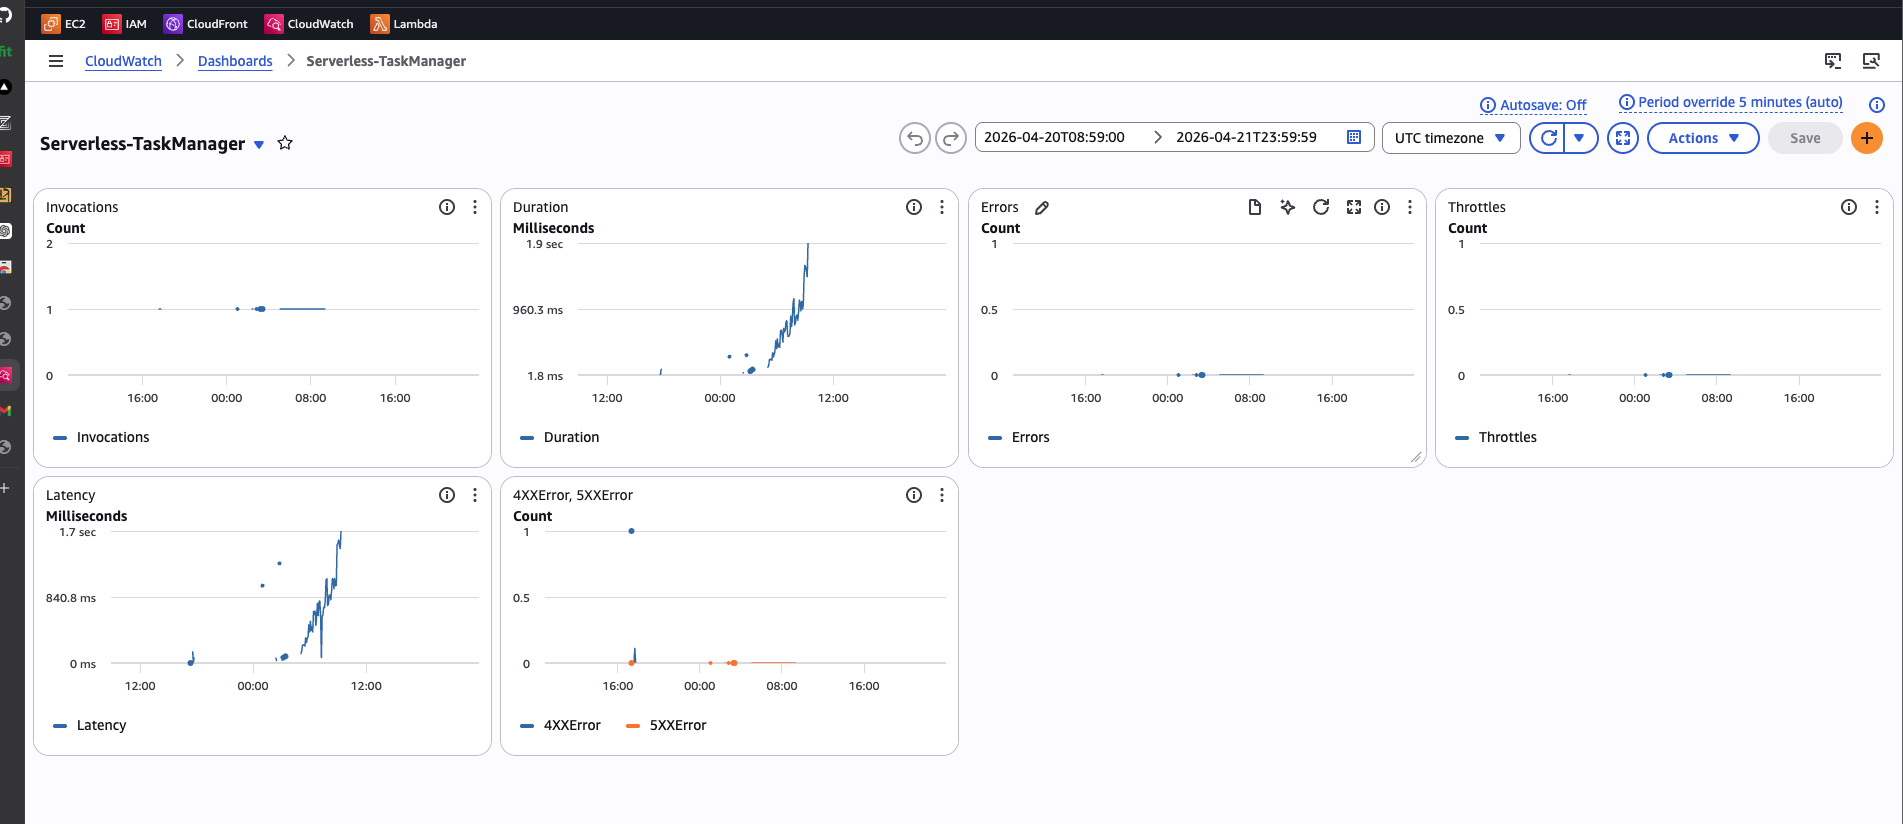
\includegraphics[width=\textwidth]{img/MON_cloudwatch_dashboard.png}
\caption{CloudWatch Dashboard với các metrics quan trọng}
\label{fig:cloudwatch_dashboard}
\end{figure}

Hình \ref{fig:cloudwatch_dashboard} cho thấy dashboard đang hoạt động với dữ liệu thực tế. Các metrics này giúp team:
\begin{itemize}
    \item Theo dõi performance và availability của hệ thống
    \item Phát hiện sớm các vấn đề tiềm ẩn
    \item Đánh giá impact của code changes
    \item Tối ưu hóa resource usage
\end{itemize}

\subsection{CloudWatch Alarms}
\label{ssec:cloudwatch_alarms}

Hệ thống được cấu hình với 2 alarms chính để phát hiện và thông báo khi có vấn đề xảy ra.

\subsubsection{Lambda Error Alarm}

\begin{itemize}
    \item \textbf{Alarm name:} Lambda-Error-Alarm
    \item \textbf{Metric:} AWS/Lambda - Errors
    \item \textbf{Condition:} Errors > 10 trong 5 phút
    \item \textbf{Action:} Gửi email qua SNS topic
    \item \textbf{Rationale:} Nếu có hơn 10 errors trong 5 phút, có thể có bug nghiêm trọng cần xử lý ngay
\end{itemize}

\subsubsection{API Gateway 5XX Alarm}

\begin{itemize}
    \item \textbf{Alarm name:} API-5xx-Alarm
    \item \textbf{Metric:} AWS/ApiGateway - 5XXError
    \item \textbf{Condition:} 5XXError > 5 trong 5 phút
    \item \textbf{Action:} Gửi email qua SNS topic
    \item \textbf{Rationale:} 5XX errors thường là server-side issues cần được xử lý ưu tiên cao
\end{itemize}

\begin{figure}[H]
\centering

\includegraphics[width=0.9\textwidth]{img/Alarm.png}
\caption{CloudWatch Alarms configuration}
\label{fig:alarms}
\end{figure}

Hình \ref{fig:alarms} hiển thị cả 2 alarms đã được cấu hình. Status có thể là:
\begin{itemize}
    \item \textbf{OK:} Metric nằm trong ngưỡng bình thường
    \item \textbf{ALARM:} Metric vượt ngưỡng, email notification được gửi
    \item \textbf{INSUFFICIENT\_DATA:} Chưa đủ dữ liệu để đánh giá
\end{itemize}

\subsubsection{SNS Email Notification}

Khi alarm được trigger, SNS gửi email notification đến team members.

\begin{figure}[H]
\centering

\includegraphics[width=0.9\textwidth]{img/Alarm-mail.png}
\caption{Email notification từ CloudWatch Alarm}
\label{fig:alarm_email}
\end{figure}

Hình \ref{fig:alarm_email} cho thấy email notification chứa:
\begin{itemize}
    \item Alarm name và description
    \item Metric details (namespace, metric name, dimensions)
    \item Threshold và actual value
    \item Timestamp khi alarm được trigger
    \item Link đến CloudWatch console để investigate
\end{itemize}

\subsection{CloudWatch Logs}
\label{ssec:cloudwatch_logs}

CloudWatch Logs tự động capture tất cả logs từ Lambda functions, giúp debugging và monitoring.

\subsubsection{Successful Request Log}

\begin{figure}[H]
\centering
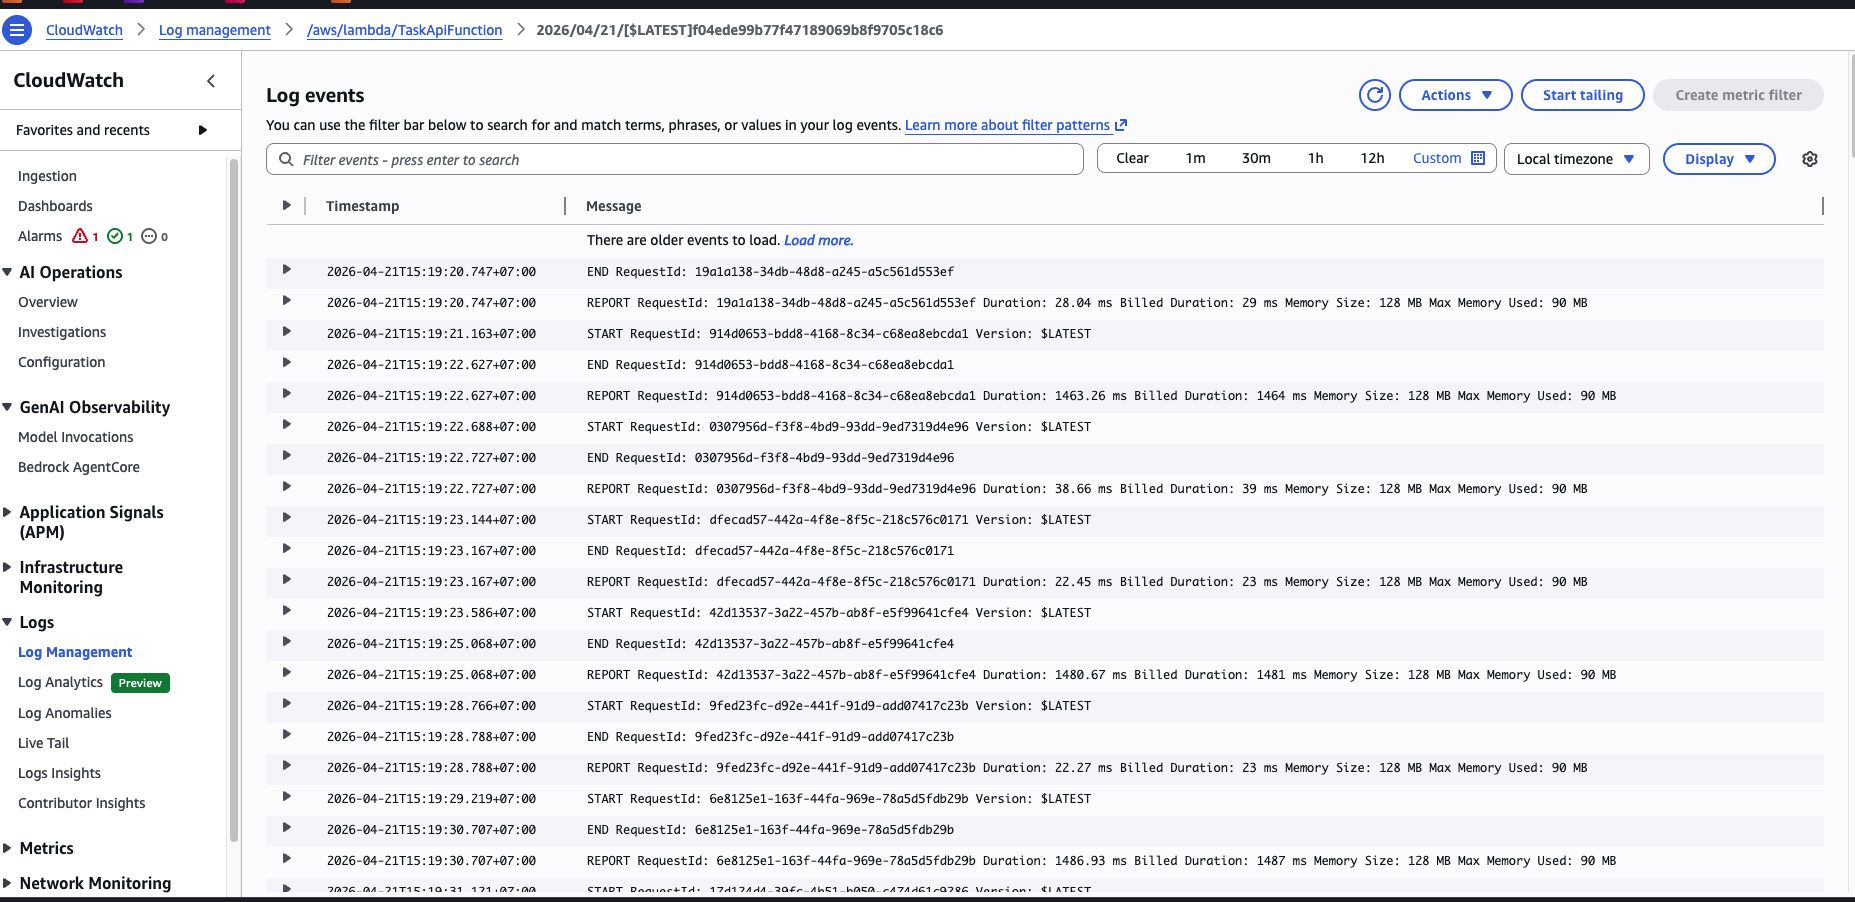
\includegraphics[width=\textwidth]{img/14-success-request.png}
\caption{CloudWatch log của successful request}
\label{fig:success_log}
\end{figure}

Hình \ref{fig:success_log} hiển thị log của một request thành công với:
\begin{itemize}
    \item \textbf{START:} Request ID và initialization
    \item \textbf{Application logs:} Custom logs từ Lambda code
    \item \textbf{REPORT:} Summary metrics
    \begin{itemize}
        \item Duration: Thời gian thực thi thực tế
        \item Billed Duration: Thời gian được tính phí (làm tròn lên 100ms)
        \item Memory Size: Memory được allocate
        \item Max Memory Used: Memory thực tế sử dụng
    \end{itemize}
\end{itemize}

\subsubsection{Error Request Log}

\begin{figure}[H]
\centering
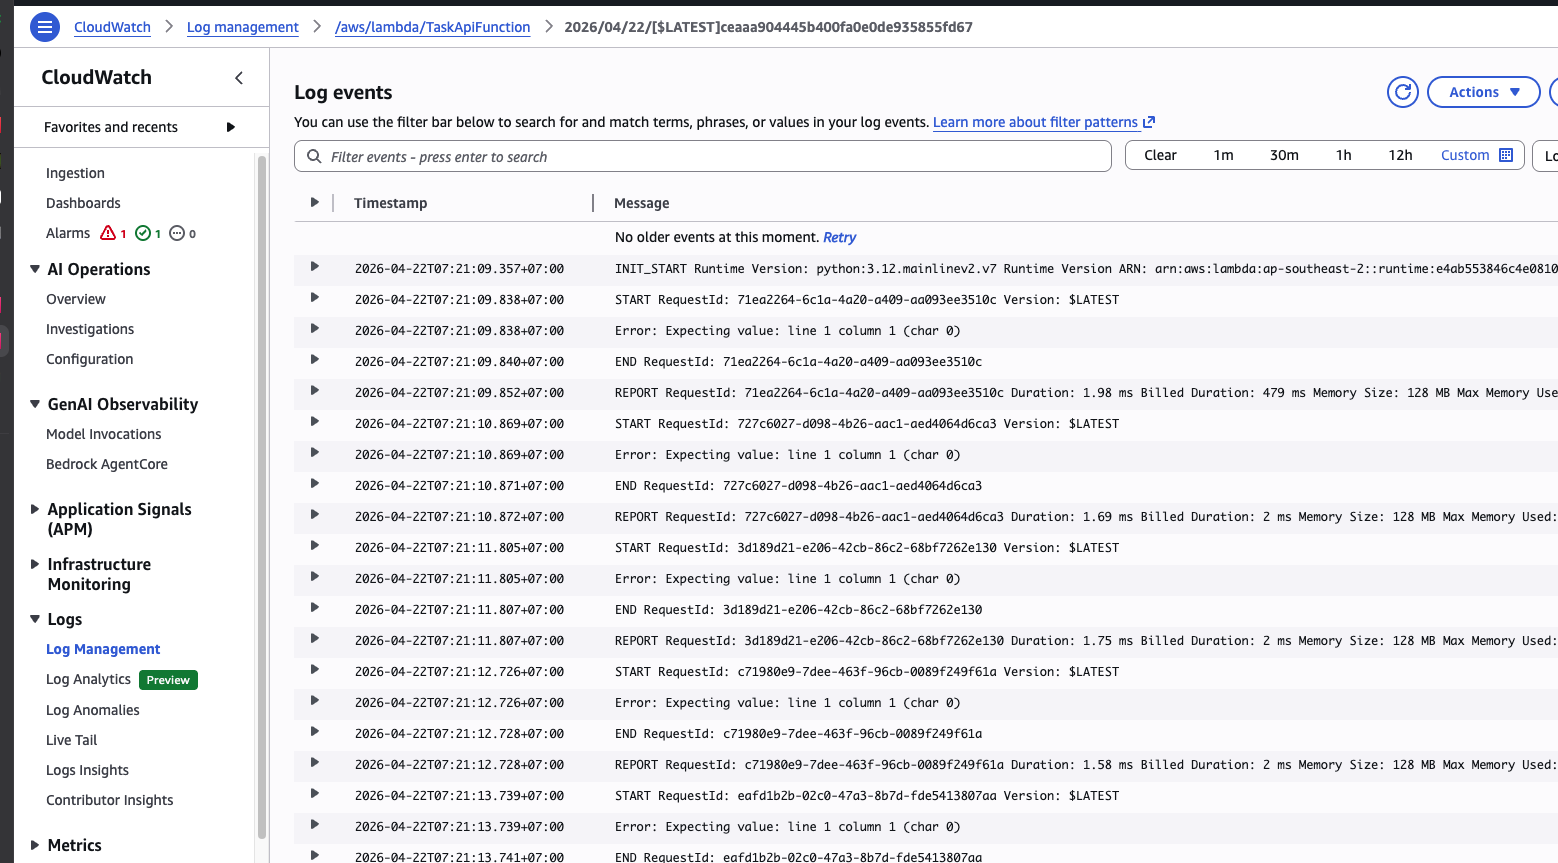
\includegraphics[width=\textwidth]{img/14-error-request.png}
\caption{CloudWatch log của error request}
\label{fig:error_log}
\end{figure}

Hình \ref{fig:error_log} cho thấy log khi có error xảy ra:
\begin{itemize}
    \item \textbf{ERROR:} Error message và stack trace
    \item \textbf{Exception details:} Type, message, và line number
    \item Giúp developers nhanh chóng identify và fix bugs
\end{itemize}

\subsection{AWS Budgets}
\label{ssec:aws_budgets}

AWS Budgets được cấu hình để kiểm soát chi phí và đảm bảo hệ thống không vượt quá Free Tier.

\subsubsection{Budget Configuration}

\begin{itemize}
    \item \textbf{Budget name:} TaskManager-Budget
    \item \textbf{Budget amount:} \$0.01 per month
    \item \textbf{Alert thresholds:}
    \begin{itemize}
        \item 80\% (\$0.008): Warning alert
        \item 100\% (\$0.01): Critical alert
    \end{itemize}
    \item \textbf{Notification:} Email qua SNS
\end{itemize}

\begin{figure}[H]
\centering
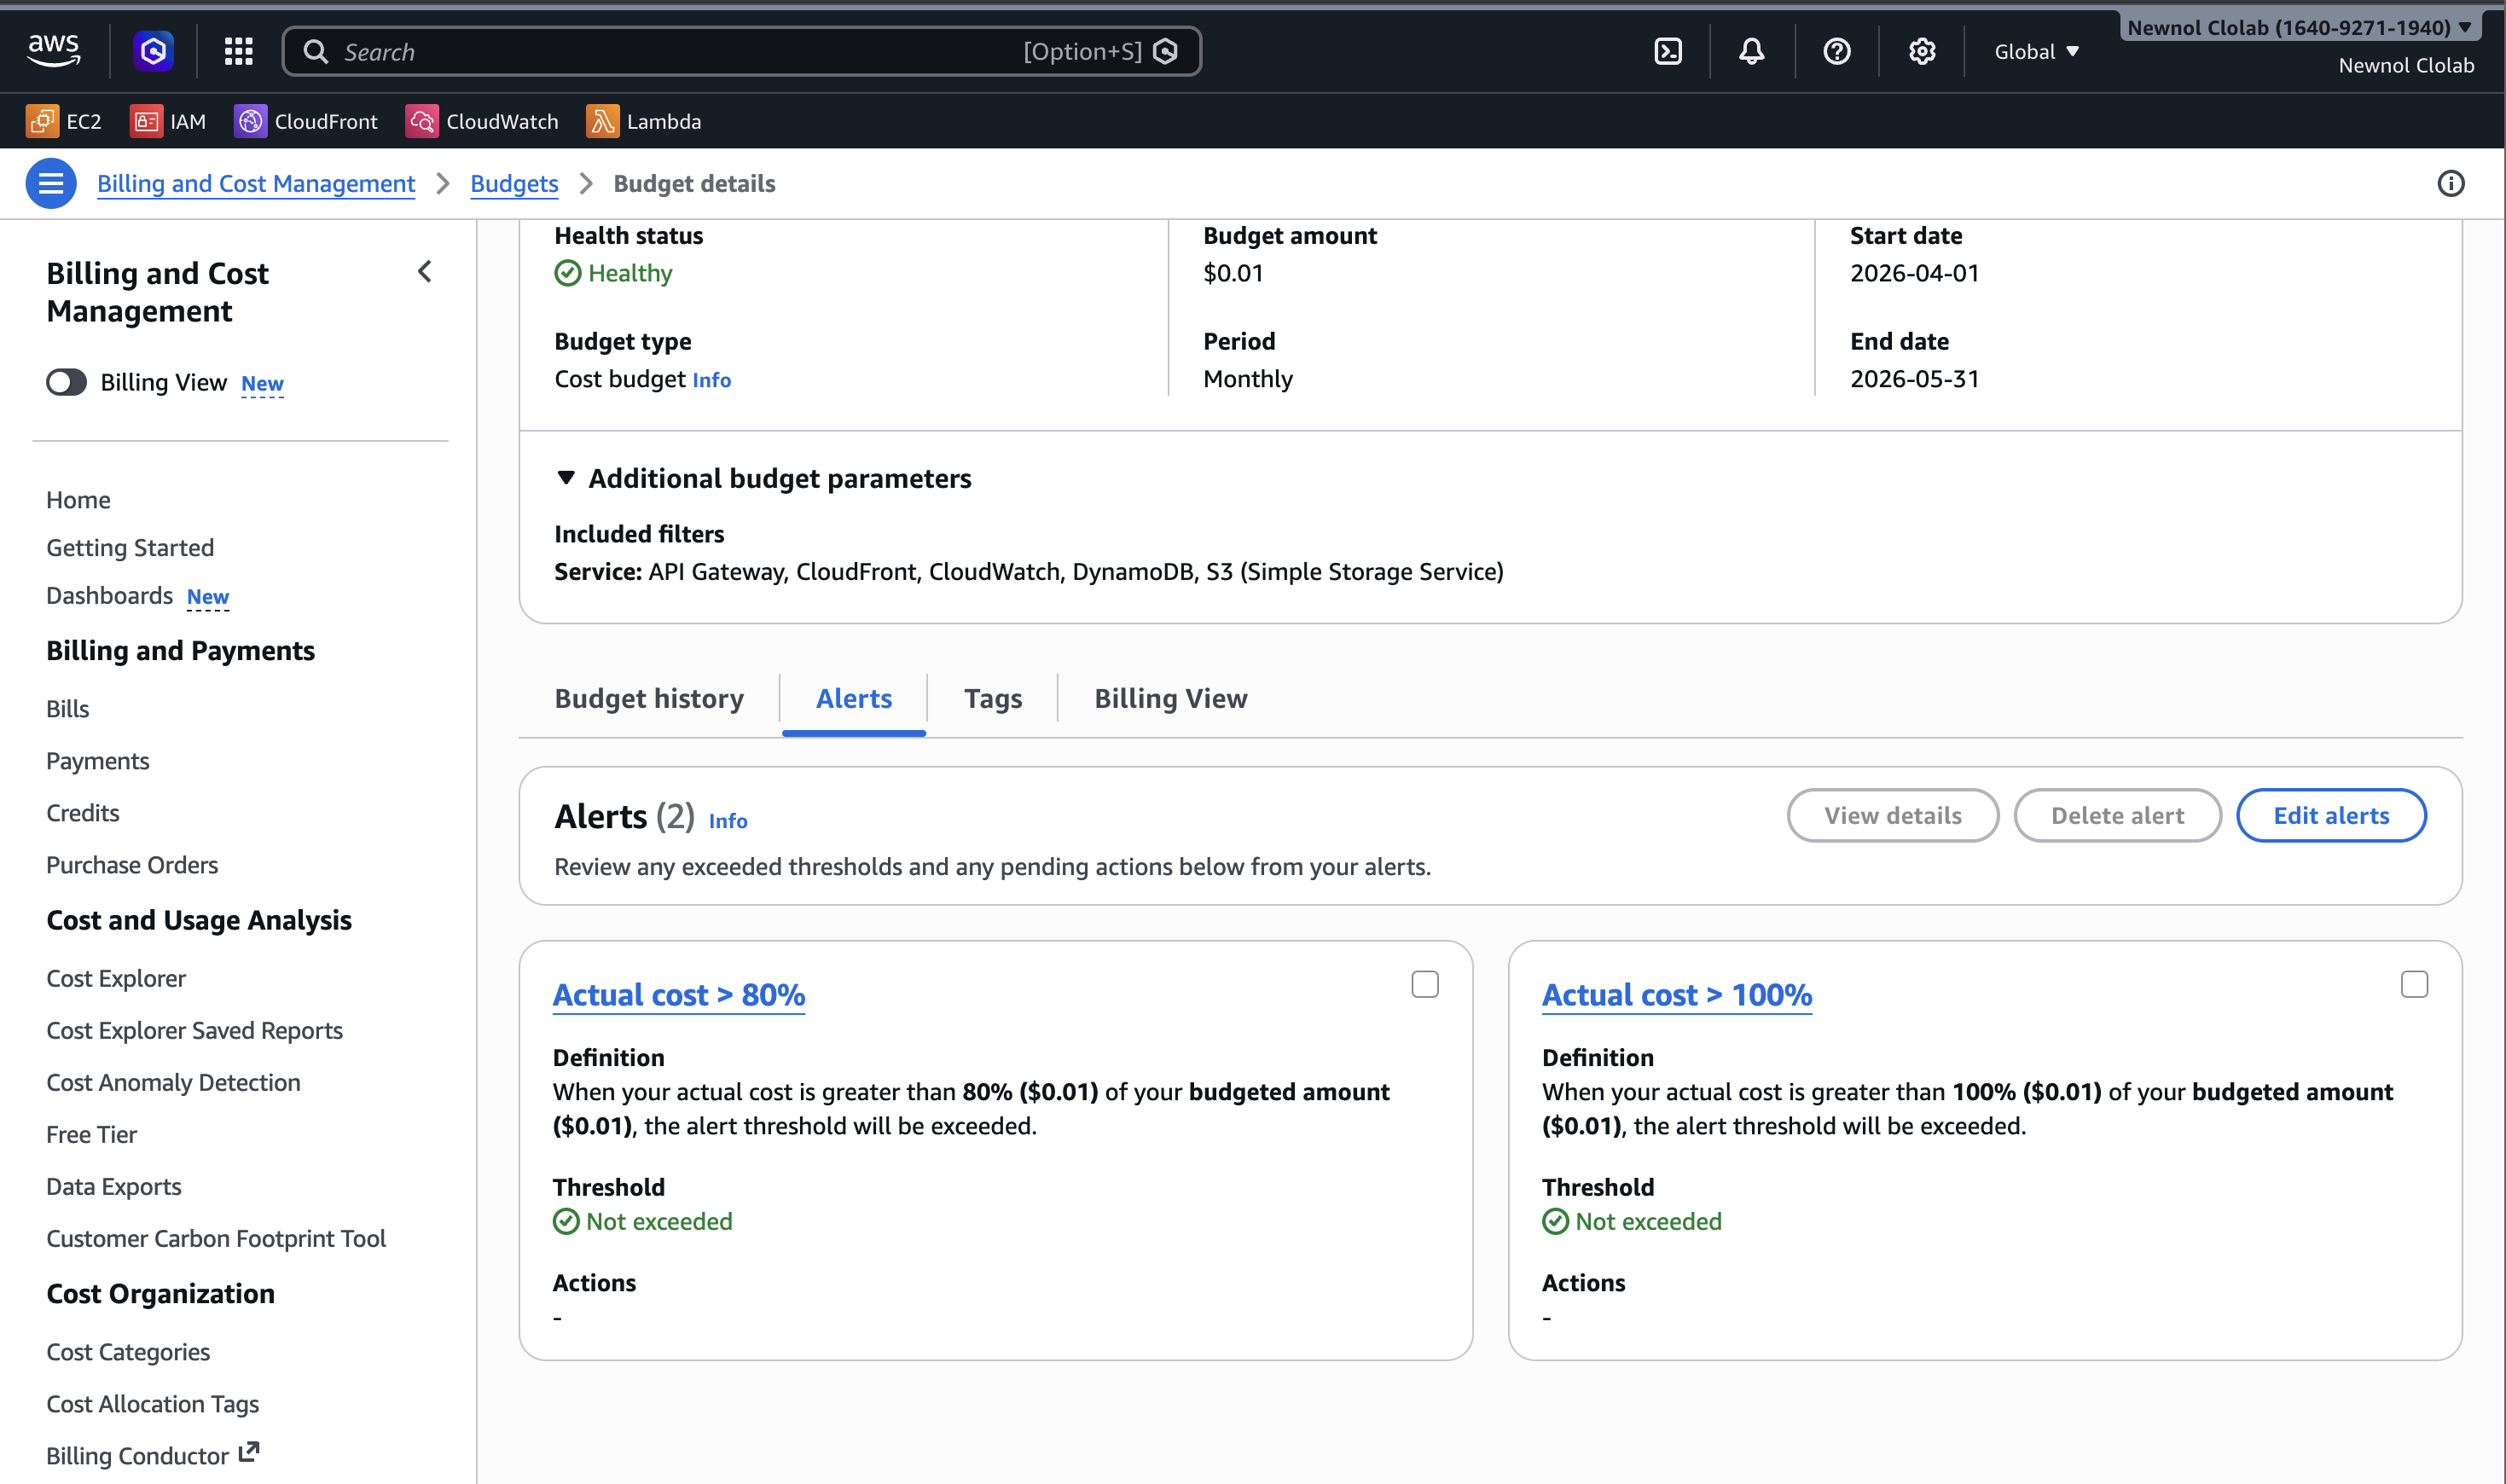
\includegraphics[width=\textwidth]{img/13-budget.png}
\caption{AWS Budgets configuration với \$0.01 limit}
\label{fig:budget}
\end{figure}

Hình \ref{fig:budget} hiển thị budget configuration. Khi chi phí đạt 80\% hoặc 100\%, email notification sẽ được gửi tự động.

\subsubsection{Budget Alert Email}

\begin{figure}[H]
\centering
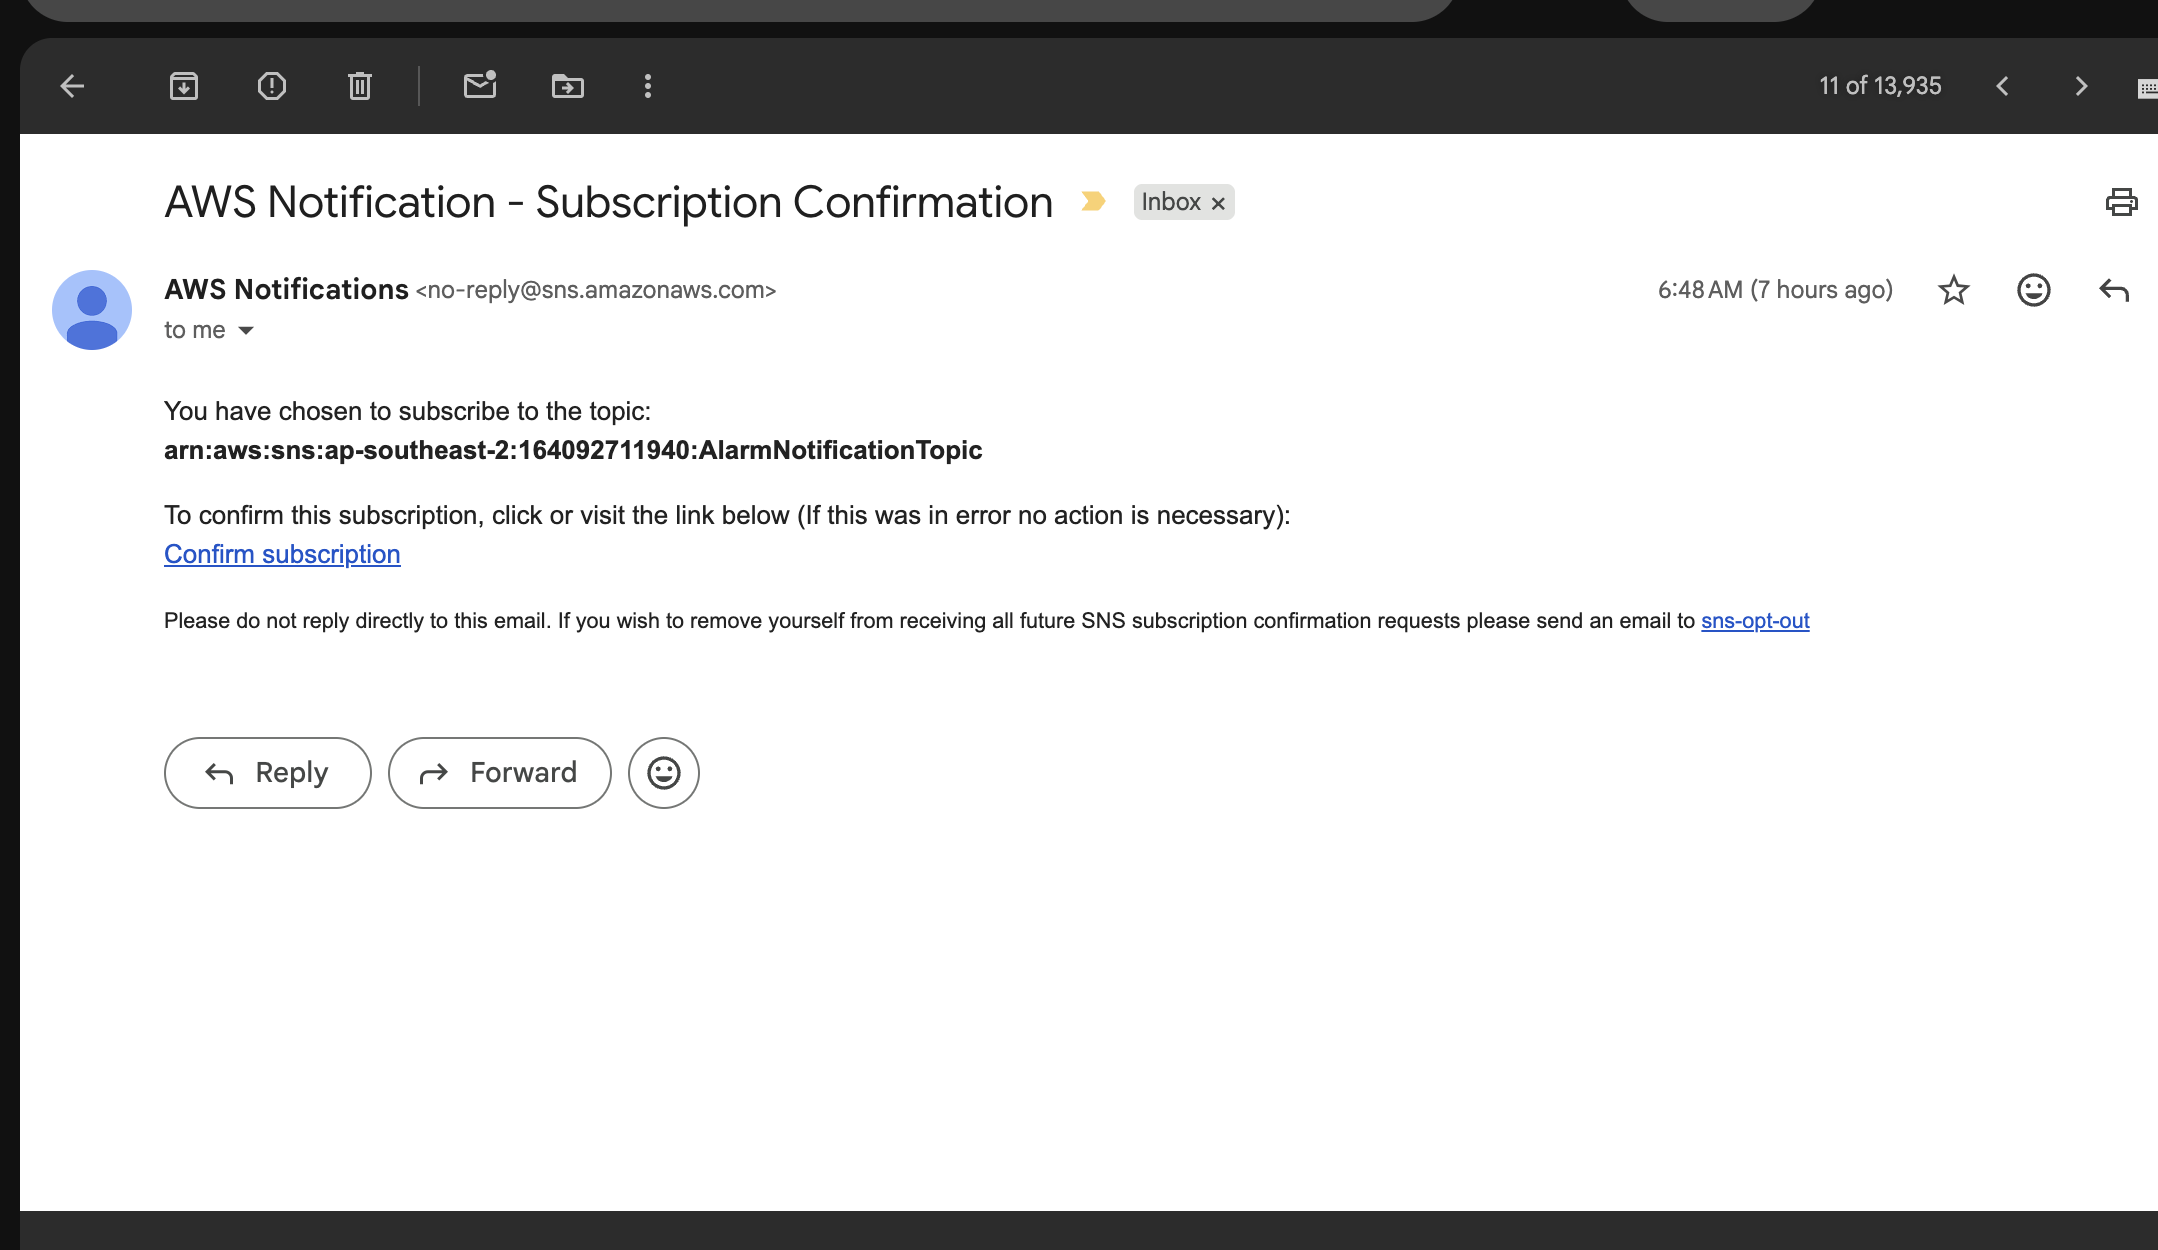
\includegraphics[width=0.9\textwidth]{img/13-email-confirm.png}
\caption{Email confirmation cho budget alerts}
\label{fig:budget_email}
\end{figure}

Hình \ref{fig:budget_email} cho thấy email subscription confirmation. Sau khi confirm, team sẽ nhận được alerts khi budget threshold được vượt qua.

\subsection{Cost Control Measures}
\label{ssec:cost_control}

Để đảm bảo chi phí bằng 0, các biện pháp sau đã được áp dụng:

\begin{table}[H]
\centering
\begin{tabular}{|l|p{6cm}|p{4cm}|}
\hline
\textbf{Service} & \textbf{Cost Control Measure} & \textbf{Free Tier Limit} \\
\hline
Lambda & Reserved Concurrency = 50 & 1M requests, 400K GB-seconds \\
\hline
API Gateway & Throttling: 100 req/s, burst 50 & 1M API calls \\
\hline
DynamoDB & On-Demand mode & 25 GB, 25 RCU/WCU \\
\hline
CloudFront & Cache optimization & 1 TB transfer, 10M requests \\
\hline
S3 & Minimal file size & 5 GB storage, 20K GET \\
\hline
VPC & No NAT Gateway, use VPC Endpoint & VPC Endpoint: Free \\
\hline
CloudWatch & Limited log retention & 5 GB logs, 10 custom metrics \\
\hline
\end{tabular}
\caption{Cost control measures cho từng service}
\label{tab:cost_control}
\end{table}

\subsection{Monitoring Best Practices}
\label{ssec:monitoring_best_practices}

Các best practices đã được áp dụng:

\begin{enumerate}
    \item \textbf{Structured Logging:} Lambda logs sử dụng JSON format để dễ dàng parse và analyze.
    
    \item \textbf{Correlation IDs:} Mỗi request có unique ID để trace qua các services.
    
    \item \textbf{Metric Dimensions:} Sử dụng dimensions để filter metrics theo function name, stage, etc.
    
    \item \textbf{Alert Fatigue Prevention:} Threshold được set hợp lý để tránh false positives.
    
    \item \textbf{Dashboard Organization:} Metrics được nhóm theo layer (API, Compute, Database).
    
    \item \textbf{Cost Monitoring:} Daily check AWS Cost Explorer để phát hiện sớm unexpected charges.
\end{enumerate}

\subsection{Tổng kết Monitoring}
\label{ssec:monitoring_summary}

Hệ thống monitoring đã được triển khai đầy đủ với:

\begin{itemize}
    \item ✓ CloudWatch Dashboard với 6+ widgets hiển thị real-time metrics
    \item ✓ 2 CloudWatch Alarms với SNS email notifications
    \item ✓ CloudWatch Logs capturing successful và error requests
    \item ✓ AWS Budgets với \$0.01 limit và 2 alert thresholds
    \item ✓ Cost control measures đảm bảo chi phí = \$0
\end{itemize}

Hệ thống monitoring này cung cấp full observability và cost control, đáp ứng đầy đủ yêu cầu của đề tài.

% \input{content/section}
% \input{content/hinhanh}
% \input{content/bangbieu}
% \input{content/congthuctoan}
% \input{content/thuattoan}
% \input{content/code}
% \input{content/ngonngu}
% \input{content/cite}

% References
\begin{thebibliography}{99}

\bibitem{aws_lambda}
Amazon Web Services,
\textit{AWS Lambda - Serverless Compute},
\url{https://aws.amazon.com/lambda/},
Accessed: 2026-04-22.

\bibitem{aws_dynamodb}
Amazon Web Services,
\textit{Amazon DynamoDB - NoSQL Database},
\url{https://aws.amazon.com/dynamodb/},
Accessed: 2026-04-22.

\bibitem{aws_vpc_endpoint}
Amazon Web Services,
\textit{VPC Endpoints - AWS PrivateLink},
\url{https://docs.aws.amazon.com/vpc/latest/privatelink/vpc-endpoints.html},
Accessed: 2026-04-22.

\bibitem{aws_cloudfront_oac}
Amazon Web Services,
\textit{Restricting access to an Amazon S3 origin with Origin Access Control},
\url{https://docs.aws.amazon.com/AmazonCloudFront/latest/DeveloperGuide/private-content-restricting-access-to-s3.html},
Accessed: 2026-04-22.

\bibitem{aws_iam_best_practices}
Amazon Web Services,
\textit{Security best practices in IAM},
\url{https://docs.aws.amazon.com/IAM/latest/UserGuide/best-practices.html},
Accessed: 2026-04-22.

\bibitem{aws_free_tier}
Amazon Web Services,
\textit{AWS Free Tier},
\url{https://aws.amazon.com/free/},
Accessed: 2026-04-22.

\bibitem{serverless_architecture}
Martin Fowler,
\textit{Serverless Architectures},
\url{https://martinfowler.com/articles/serverless.html},
2016.

\bibitem{aws_well_architected}
Amazon Web Services,
\textit{AWS Well-Architected Framework},
\url{https://aws.amazon.com/architecture/well-architected/},
Accessed: 2026-04-22.

\end{thebibliography}


% Appendix
% Add \cleardoublepage to move appendices to next page.
\cleardoublepage
\appendix

\section{Hướng dẫn triển khai}
\label{apd:deployment}

\subsection{Yêu cầu hệ thống}
\label{ssec:requirements}

Trước khi bắt đầu triển khai, đảm bảo bạn đã có:

\begin{itemize}
    \item AWS Account với Free Tier available
    \item AWS CLI đã được cài đặt và cấu hình
    \item Python 3.12 hoặc cao hơn
    \item Git để clone source code
    \item Text editor hoặc IDE (VS Code, PyCharm, etc.)
\end{itemize}

\subsection{Bước 1: Tạo VPC và Network Infrastructure}
\label{ssec:deploy_vpc}

\subsubsection{Tạo VPC}

\begin{verbatim}
aws ec2 create-vpc \
  --cidr-block 10.0.0.0/16 \
  --tag-specifications 'ResourceType=vpc,Tags=[{Key=Name,Value=TaskManager-VPC}]'
\end{verbatim}

Lưu lại VPC ID từ output.

\subsubsection{Enable DNS}

\begin{verbatim}
aws ec2 modify-vpc-attribute \
  --vpc-id <VPC_ID> \
  --enable-dns-hostnames

aws ec2 modify-vpc-attribute \
  --vpc-id <VPC_ID> \
  --enable-dns-support
\end{verbatim}

\subsubsection{Tạo Private Subnets}

\begin{verbatim}
# Subnet A
aws ec2 create-subnet \
  --vpc-id <VPC_ID> \
  --cidr-block 10.0.1.0/24 \
  --availability-zone ap-southeast-1a \
  --tag-specifications 'ResourceType=subnet,Tags=[{Key=Name,Value=Private-Subnet-A}]'

# Subnet B
aws ec2 create-subnet \
  --vpc-id <VPC_ID> \
  --cidr-block 10.0.2.0/24 \
  --availability-zone ap-southeast-1b \
  --tag-specifications 'ResourceType=subnet,Tags=[{Key=Name,Value=Private-Subnet-B}]'
\end{verbatim}

\subsubsection{Tạo Route Table}

\begin{verbatim}
aws ec2 create-route-table \
  --vpc-id <VPC_ID> \
  --tag-specifications 'ResourceType=route-table,Tags=[{Key=Name,Value=Private-RT}]'

# Associate với subnets
aws ec2 associate-route-table \
  --route-table-id <RT_ID> \
  --subnet-id <SUBNET_A_ID>

aws ec2 associate-route-table \
  --route-table-id <RT_ID> \
  --subnet-id <SUBNET_B_ID>
\end{verbatim}

\subsubsection{Tạo VPC Endpoint cho DynamoDB}

\begin{verbatim}
aws ec2 create-vpc-endpoint \
  --vpc-id <VPC_ID> \
  --service-name com.amazonaws.ap-southeast-1.dynamodb \
  --route-table-ids <RT_ID>
\end{verbatim}

\subsubsection{Tạo Security Group}

\begin{verbatim}
aws ec2 create-security-group \
  --group-name lambda-sg \
  --description "Security group for Lambda functions" \
  --vpc-id <VPC_ID>

# Add outbound rule cho DynamoDB
aws ec2 authorize-security-group-egress \
  --group-id <SG_ID> \
  --ip-permissions IpProtocol=tcp,FromPort=443,ToPort=443,PrefixListIds=[{PrefixListId=<DDB_PREFIX_LIST>}]
\end{verbatim}

\subsection{Bước 2: Tạo DynamoDB Table}
\label{ssec:deploy_dynamodb}

\begin{verbatim}
aws dynamodb create-table \
  --table-name Tasks \
  --attribute-definitions \
    AttributeName=taskId,AttributeType=S \
    AttributeName=userId,AttributeType=S \
    AttributeName=createdAt,AttributeType=S \
  --key-schema AttributeName=taskId,KeyType=HASH \
  --billing-mode PAY_PER_REQUEST \
  --global-secondary-indexes \
    "[{\"IndexName\":\"userId-index\",\"KeySchema\":[{\"AttributeName\":\"userId\",\"KeyType\":\"HASH\"},{\"AttributeName\":\"createdAt\",\"KeyType\":\"RANGE\"}],\"Projection\":{\"ProjectionType\":\"ALL\"}}]"
\end{verbatim}

\subsection{Bước 3: Tạo IAM Role cho Lambda}
\label{ssec:deploy_iam}

\subsubsection{Tạo Trust Policy}

Tạo file \texttt{trust-policy.json}:

\begin{verbatim}
{
  "Version": "2012-10-17",
  "Statement": [
    {
      "Effect": "Allow",
      "Principal": {"Service": "lambda.amazonaws.com"},
      "Action": "sts:AssumeRole"
    }
  ]
}
\end{verbatim}

\subsubsection{Tạo Permissions Policy}

Tạo file \texttt{lambda-policy.json}:

\begin{verbatim}
{
  "Version": "2012-10-17",
  "Statement": [
    {
      "Effect": "Allow",
      "Action": [
        "dynamodb:GetItem",
        "dynamodb:PutItem",
        "dynamodb:UpdateItem",
        "dynamodb:DeleteItem",
        "dynamodb:Query",
        "dynamodb:Scan"
      ],
      "Resource": [
        "arn:aws:dynamodb:ap-southeast-1:<ACCOUNT_ID>:table/Tasks",
        "arn:aws:dynamodb:ap-southeast-1:<ACCOUNT_ID>:table/Tasks/index/*"
      ]
    },
    {
      "Effect": "Allow",
      "Action": [
        "logs:CreateLogGroup",
        "logs:CreateLogStream",
        "logs:PutLogEvents"
      ],
      "Resource": "arn:aws:logs:*:*:*"
    },
    {
      "Effect": "Allow",
      "Action": [
        "ec2:CreateNetworkInterface",
        "ec2:DescribeNetworkInterfaces",
        "ec2:DeleteNetworkInterface"
      ],
      "Resource": "*"
    }
  ]
}
\end{verbatim}

\subsubsection{Tạo Role}

\begin{verbatim}
aws iam create-role \
  --role-name LambdaTaskRole \
  --assume-role-policy-document file://trust-policy.json

aws iam put-role-policy \
  --role-name LambdaTaskRole \
  --policy-name LambdaTaskPolicy \
  --policy-document file://lambda-policy.json
\end{verbatim}

\subsection{Bước 4: Deploy Lambda Function}
\label{ssec:deploy_lambda}

\subsubsection{Chuẩn bị code}

\begin{verbatim}
# Clone repository
git clone <REPO_URL>
cd aws-zerocost-serverless/backend

# Package Lambda function
zip -r lambda.zip lambda_function.py
\end{verbatim}

\subsubsection{Create Lambda Function}

\begin{verbatim}
aws lambda create-function \
  --function-name TaskApiFunction \
  --runtime python3.12 \
  --role arn:aws:iam::<ACCOUNT_ID>:role/LambdaTaskRole \
  --handler lambda_function.lambda_handler \
  --zip-file fileb://lambda.zip \
  --timeout 30 \
  --memory-size 128 \
  --vpc-config SubnetIds=<SUBNET_A_ID>,<SUBNET_B_ID>,SecurityGroupIds=<SG_ID> \
  --reserved-concurrent-executions 50
\end{verbatim}

\subsection{Bước 5: Tạo API Gateway}
\label{ssec:deploy_apigw}

\subsubsection{Tạo REST API}

\begin{verbatim}
aws apigateway create-rest-api \
  --name TaskManagerAPI \
  --description "API for Task Manager application"
\end{verbatim}

\subsubsection{Tạo Resources và Methods}

Sử dụng AWS Console hoặc AWS CLI để:
\begin{enumerate}
    \item Tạo resource /tasks
    \item Tạo resource /tasks/\{id\}
    \item Tạo methods: GET, POST, PUT, DELETE
    \item Configure Lambda integration
    \item Enable CORS
    \item Deploy to prod stage
\end{enumerate}

\subsection{Bước 6: Deploy Frontend}
\label{ssec:deploy_frontend}

\subsubsection{Tạo S3 Bucket}

\begin{verbatim}
aws s3 mb s3://task-manager-frontend-<UNIQUE_ID>

# Enable Block Public Access
aws s3api put-public-access-block \
  --bucket task-manager-frontend-<UNIQUE_ID> \
  --public-access-block-configuration \
    "BlockPublicAcls=true,IgnorePublicAcls=true,BlockPublicPolicy=true,RestrictPublicBuckets=true"
\end{verbatim}

\subsubsection{Upload Frontend Files}

\begin{verbatim}
cd ../frontend
aws s3 sync . s3://task-manager-frontend-<UNIQUE_ID>/
\end{verbatim}

\subsubsection{Tạo CloudFront Distribution}

Sử dụng AWS Console để:
\begin{enumerate}
    \item Tạo CloudFront distribution
    \item Origin: S3 bucket
    \item Origin Access: OAC
    \item Default root object: index.html
    \item Deploy và đợi distribution active
\end{enumerate}

\subsubsection{Update S3 Bucket Policy}

Copy bucket policy từ CloudFront và apply vào S3 bucket.

\subsection{Bước 7: Setup Monitoring}
\label{ssec:deploy_monitoring}

\subsubsection{Tạo SNS Topic}

\begin{verbatim}
aws sns create-topic --name TaskManager-Alerts

aws sns subscribe \
  --topic-arn <TOPIC_ARN> \
  --protocol email \
  --notification-endpoint your-email@example.com
\end{verbatim}

Confirm email subscription.

\subsubsection{Tạo CloudWatch Alarms}

\begin{verbatim}
# Lambda Error Alarm
aws cloudwatch put-metric-alarm \
  --alarm-name Lambda-Error-Alarm \
  --alarm-description "Alert when Lambda errors exceed threshold" \
  --metric-name Errors \
  --namespace AWS/Lambda \
  --statistic Sum \
  --period 300 \
  --evaluation-periods 1 \
  --threshold 10 \
  --comparison-operator GreaterThanThreshold \
  --alarm-actions <SNS_TOPIC_ARN>

# API Gateway 5XX Alarm
aws cloudwatch put-metric-alarm \
  --alarm-name API-5xx-Alarm \
  --alarm-description "Alert when API 5XX errors exceed threshold" \
  --metric-name 5XXError \
  --namespace AWS/ApiGateway \
  --statistic Sum \
  --period 300 \
  --evaluation-periods 1 \
  --threshold 5 \
  --comparison-operator GreaterThanThreshold \
  --alarm-actions <SNS_TOPIC_ARN>
\end{verbatim}

\subsubsection{Tạo AWS Budget}

Sử dụng AWS Console:
\begin{enumerate}
    \item Navigate to AWS Budgets
    \item Create budget với amount \$0.01
    \item Set alerts at 80\% và 100\%
    \item Add email notification
\end{enumerate}

\subsection{Bước 8: Testing}
\label{ssec:testing}

\subsubsection{Test API Endpoints}

\begin{verbatim}
# Test GET /tasks
curl https://<API_ID>.execute-api.ap-southeast-1.amazonaws.com/prod/tasks

# Test POST /tasks
curl -X POST https://<API_ID>.execute-api.ap-southeast-1.amazonaws.com/prod/tasks \
  -H "Content-Type: application/json" \
  -d '{"userId":"user1","title":"Test Task","priority":"high","dueDate":"2026-05-01"}'
\end{verbatim}

\subsubsection{Test Frontend}

Truy cập CloudFront URL: https://<DISTRIBUTION_ID>.cloudfront.net

\subsection{Troubleshooting}
\label{ssec:troubleshooting}

\subsubsection{Lambda không kết nối được DynamoDB}

\begin{itemize}
    \item Kiểm tra VPC Endpoint đã được tạo chưa
    \item Kiểm tra Route Table có route đến VPC Endpoint
    \item Kiểm tra Security Group cho phép outbound port 443
    \item Kiểm tra IAM Role có quyền DynamoDB
\end{itemize}

\subsubsection{CloudFront không truy cập được S3}

\begin{itemize}
    \item Kiểm tra OAC đã được attach
    \item Kiểm tra S3 Bucket Policy cho phép CloudFront
    \item Đợi CloudFront distribution deploy xong (15-20 phút)
\end{itemize}

\subsubsection{Lambda cold start chậm}

\begin{itemize}
    \item Tăng memory size (tăng memory cũng tăng CPU)
    \item Sử dụng Provisioned Concurrency (nhưng tốn phí)
    \item Optimize code để giảm dependencies
\end{itemize}

\subsection{Source Code Repository}
\label{ssec:source_code}

Source code đầy đủ có tại: \url{https://github.com/your-repo/aws-zerocost-serverless}

Cấu trúc thư mục:
\begin{verbatim}
aws-zerocost-serverless/
├── frontend/
│   ├── index.html
│   ├── style.css
│   └── app.js
├── backend/
│   └── lambda_function.py
├── infra/
│   ├── vpc.yaml
│   └── dynamodb.yaml
└── docs/
    └── architecture_v3.png
\end{verbatim}

\end{document}